\documentclass[a4paper,12pt]{book}
\usepackage{amsmath}
\usepackage{hyperref} % For creating hyperlinks in cross references
\usepackage{graphicx} % Packages to allow inclusion of graphics (PNG)
\usepackage{rotating} % for putting pictures sideways
\usepackage{multirow} 
\usepackage{framed}
\usepackage{longtable}
\usepackage[T4]{fontenc}
\usepackage{devanagari}

%\usepackage{polyglossia}
%\setdefaultlanguage[variant=american]{english}
%\usepackage{mathpazo}
%\usepackage{txfonts}


\parindent 0cm % Override the left margin to 0 cm.
\parskip 0.2cm
\topmargin 0.2cm
\oddsidemargin 0.5cm %1cm
\evensidemargin 0.5cm
\textwidth 15cm
\textheight 21cm

%\def\R{\mathbb{ R}}
%\def\S{\mathbb{ S}}
%\def\I{\mathbb{ I}}
\makeindex
%\title{Cultural Heritage of the Dhati People of Thar Desert}
%\author{Translation of the original work titled\\ ``Our Cultural Heritage" by Bansidhar Maheshwari\\ from Gujarati to English by Dr. Ketan C. Maheshwari}
%\date{}

\begin{document}

%%%%%%%
\clearpage
%% temporary titles
% command to provide stretchy vertical space in proportion
\newcommand\nbvspace[1][3]{\vspace*{\stretch{#1}}}
% allow some slack to avoid under/overfull boxes
\newcommand\nbstretchyspace{\spaceskip0.5em plus 0.25em minus 0.25em}
% To improve spacing on titlepages
\newcommand{\nbtitlestretch}{\spaceskip0.6em}
%\pagestyle{empty}
\begin{center}
\bfseries
\nbvspace[1]
\Huge
{\nbtitlestretch\huge
CULTURAL HERITAGE OF THE DHATI PEOPLE}

\nbvspace[1]
\normalsize

Translation of the original work titled\\ ``Our Cultural Heritage" by Bansidhar Maheshwari\\ from Gujarati to English 
\nbvspace[1]
\small by\\
\small DR. KETAN C. MAHESHWARI\\[0.5em]

\nbvspace[2]

%\includegraphics[width=1.5in]{./graphics/pic37}
\nbvspace[3]
\normalsize

CHICAGO\\
\large
TO BE PUBLISHED
\nbvspace[1]
\end{center}

%%%%%%%

%\maketitle
\let\cleardoublepage\clearpage
\tableofcontents
\chapter*{Preface by the Translator}

Presenting the English translation of the unique work by Bansidhar Maheshwari
documenting the cultural heritage of the Dhati people of Thar desert. Dhati and
Maheshwari are used interchangeably in places. Attempted to do a literal
translation where possible. In other places a translation is done with the most
appropriate interpretation. Apologize for any mistakes. Please send your
feedback to ketancmaheshwari@gmail.com. Notations: Words/statements in Gujarati
are noted in \textit{italics} and Dhati language in \textbf{bold}.  Hope you
find the book informative.

--
Ketan
July 2016

\chapter*{Pronunciation Guide}

The book is full of non-English words from Dhati-Thari, and Gujarati language. Some
Sindhi and Hindi words too appear occasionally. An attempt is made to use
special accented letters so that reader is able to pronounce them correctly.
Table~\ref{tbl:pronunciation} shows the pronunciation of various accented
letters used through the book.

\begin{table}
\begin{center}
% use packages: array
\begin{tabular}{|l|l|l|l|}
\hline
\textbf{term} & \textbf{equivalent Gujarati character}  & \textbf{example} & \textbf{pronounced-as} \\
\hline
\"{a} &  &  & father \\
\"{d} &  &  & d\M{e} \\
\hline

\hline
\end{tabular}
\end{center}
\caption{Pronunciation Guide}
\label{tbl:pronunciation}
\end{table}


\chapter{The Origin of the Dhati Community}
\chaptermark{Origin}
Authentic historical literature about the origin of the Maheshwari community is not available. The sole source of information available is in the form of a book ``Itihas Kalpdrum Maheshwari Kulbhushan'' authored by late Shivkaranji Darak of Mundwa. Based on the book, following is the description of the origins of the Maheshwari community:

Suryawanshi King Khadgalsen of Chauhan dynasty was ruling over Khandelanagar state. He was very kind and just king. People lived happily and peacefully in his kingdom. He was always worried of not having a son.

One day the king had invited Brahmins and paid great honour to them. The Brahmins were very happy with the king's courtesy and asked him for a boon. The king then expressed his desire for a son. Brahmins said, ``if you worship Lord Shiva, you will be blessed with a very brave and adventurous son, but do not allow him to go towards the north and take bath in the Surya-kund there until he turns 16 years old". If the prince respects Brahmins, he will become a great king else will be reborn in the same kingdom. Hence being blessed by the Brahmins, the king rewarded them with fine clothes and jewelry and respectfully saw them off. The king worshipped God Shiva and was blessed with the boon.

King Khadgalsen had 24 queens. After some time, one of the queens, Champawati gave birth to a baby boy. The king was very happy and named the prince as Sujan Kunwar. The prince learned horse-riding, weapons etc. by the age 7 years. When he reached the age of 12, enemies were afraid of him. The king was quite satisfied with his work. He was careful not to let the prince go towards the North.

Once a Jain sadhu came and preached the prince about Jain religion luring him into anti-Shiva beliefs and showed the faults of Brahmins. At the age of 14, the prince opposed Shiva and started practicing Jain religion. He campaigned the Jain religion in East, West and South and banished idol worshipping. He used to harass Brahmins and broke their sacred threads (\textit{janoi}). He forbade all religious activities including yajna and hawana. Out of the King's fear, he never went towards the North direction, but who can stop the destiny.

Once he went towards the North to the Suryakund with his 72 officers. He had grown angry when he saw 6 Rishis performing a yajna. He ordered his officers to destroy the yajna and harassed the rishis. Seeing this the rishis cursed them to become stone-like. So the prince including all his officers and horses became stone-like. This news spread very quickly in all directions.

The King and citizens became worried after hearing this news. King Khadgalsen died of the shock. 16 of his queens became \textit{sati} with him. With no protector of the kingdom, neighbouring enemies attacked the state. They divided the state into many regions and merged them into their own states.

Even as this happened, the prince's widow and 72 officer's widows cried and went to the rishis. They humbly requested and begged for the lives of their husbands. Seeing this rishi went soft. However, they said they are not capable enough of revert the curse. They advised the ladies to go to a nearby cave and worship God Shiva so that the curse can be taken off. All the ladies went to a cage and religiously meditated for appeasement of God Shiva.

After some time, God Shiva and Parvatiji came around the place where the prince and officers were lying stone-like. Parvatiji asked what happened and Shivji told the whole history.

At this time the prince's queen and the officer's wives fell on the feet of Parvatiji and expressed their plight. Seeing this, Parvatiji requested Shivji of taking off the curse. God taken off the curse and freed them of the stone-like state giving them a new life. Everybody fell on the God's feet.

As the prince became conscious, his mind filled with lust seeing Parvatiji's beauty. Seeing this Parvatiji cursed the prince like this: ``O bad man! you will always beg for food and your all coming generations shall beg for food''! These people were called ``jaaga'' (bhat) later on.

The 72 officers said: ``O God! Now we do not have a place to live. What should we do now''? So Shivji informed them, that they quit their Kshatriya religion in a previous birth so now they are liable to accept the Vaishya religion. Go to the Suryakund and have bath. As they bathed, their sword became pen, sword-case became stick and shields became weighing balance. All officers became Vaishya. As God Mahesh gave them lesson, they were called ``\textbf{Maheshwari}'' Vaishya.

When rishis came to know that everybody has been freed of curse, they asked God: ``O God! how will our incomplete Yajna will be completed''? Hence God preached to the officers that now onwards these rishis are your guru and you accept them as such. God told the rishis that they do not have anything as of now but when they have some occasion in their home they will give you material things to the best of their capabilities. You should teach them to follow their religion. Rishi accepted them as their pupils and each rishi accepted 12 pupils. Following is their description: 
(1) Parik from Parashar rishi (2) Dadma from Dadhichi rishi (3) Adigol from Gautam rishi (4) Khandelwal from Kharik rishi (5) Sukuwal from Sukumarg rishi (6) Saraswat brahmin/purohit from Sarasur rishi.

After some time of leaving Khandela all settled in Didwana. From these 72 officers, 72 \textit{nukhs (clans)} came into existence and from these \textit{nukhs}, depending upon the business, \textit{peta-nukhs} came into existence.

This day was the ninth day of \textit{Jeth-sud} month. This day is celebrated as \textbf{``Mahesh Navami''} in all over India by Maheshwaris. Maheshwari community is progressing continuously.

\chapter{Amazing Life-Journey of the Maheshwari Community}
Quitting the Kshatriya religion and accepting the pen and weighing-balance is as courageous and amazing story of the King's officers as is the story of the life-journey of the Maheshwari community.

The origin of Maheshwari community is Marwad region, but being a deserted region and as lack of enough rains they had to face droughts year after year. Such a situation made the life of Maheshwari families very difficult. In such conditions, life became a challenge for them and they decided to face it with exceptional courage. They made small groups and went out of their region in order to search for their bread-butter and employment.

So, some went to Mewad and others to Jaipur via Ajmer. Yet others went to Bikaner, crossing Jodhpur border to Pokhran, falaudi, Jaisalmer, Barmer, Sindh, Kutchch, Jamnagar etc. places.

According to some Historians, families from Jaisalmer migrated and settled in Gujarat in the 13th century A.D.. Families from Mewad went ahead towards Maharashtra via Gujarat, Jaipur families went towards Delhi, and that ofBikaner went to Calcutta crossing many many borders. People from Marwar also went to Mumbai and Maharashtra. This flow continued for a long time and many family went and settled in Bengal and current Bangladesh as well. People from Jodhpur region went towards Bihar and Assam and then to Utkal-Assam and Nagaland. Some of the Maheshwari people from the Purania district of Bihar started going to the weekly market at Viratnagar (currently Nepalgunj in Nepal) and got settled there.

One group of Jaisalmer went to Malwa in Central India and Vidarbh via east Madhya Pradesh's Gondwana (Jabalpur etc.) and another group went and settled in Uttar Pradesh's Mathura, Aligarh, Kaasgunj, Meerut and Saharanpur. Such was the journey of the community and went on to spread in a large portion of the country, providing a courageous example like other Vaishya communities of Rajasthan.

For the above mentioned expansion, apart from livelihood, self and family's safety and security was also a reason. Muslim era -- from Allauddin Khilji to Aurangzeb -- from around year 1300 A.D. till year 1700 A.D. -- 400 years and Maratha civil war were also responsible for such migrations.

Today Maheshwari community is not only settled in India but have crossed international borders as well. With today's transportation and communication facilities it is not very much surprising that people migrate to different countries but imagining how our ancestors used to protect their families of thieves-dacoits and enemies using those primitive tools will give goose-bumps to the most courageous of today's people. We can but only imagine how by foot, camel and ox-carts, they migrated to unknown regions, mixed with strange people, adapted their unknown language and customs and demonstrated great courage. Such people with their self-courage and firm determination accepted and faced all kinds of adversities and eventually reached on top successfully.

Today we are tasting sweet consequences of our ancestors holy courage. It is very satisfying that even today we remain firm in different situations and face various challenges in order to keep the name of our community high and have a bright future. Fresh instances of this courage is our maigrations during the 1947 partition and then 1971 war and migrations between 1988-92.

Currently, many Maheshwaris live outside of India of which following are main countries:
\begin{center}
% use packages: array
\begin{tabular}{ll}
America, Canada and Britain & Approx. 150 to 200 families \\ 
Nepal & Approx. 200 to 250 families \\ 
Bangladesh & Approx. 300 to 400 families \\ 
Sindh (Pakistan) & Approx. 600 to 700 families
\end{tabular}
\end{center}

In the evolution of Maheshwari community it is important to note that they started with 72 branches that have increased because of various reasons and now they are approximately 80.

Depending upon the contemporary requirements, keeping away from the fame, using wisdom, farsighted decision-making is still a lesson for the new generation as much as it is a requirement of the future.
\chapter{Migration from Marwar to Thar}
As mentioned in earlier chapter, the Maheshwari community migrated from Jaisalmer to different parts of India between A.D. 1300 and A.D. 1700 because of different causes. Main reasons for these migrations might be Muslim tyranny, Maratha civil war and continuous drought etc.. ( Only those who had to leave their age-old home and country can know the pain and agony they had to undergo!)

While migrating, where to go was a question. A safe and known place would be a natural choice. Royal states of Jaisalmer and Amarkot (Umarkot) were connected through marriage relationships as the following examples shows:
\begin{enumerate}
 \item Jaisalmer's king Chachakdev first married Umarkot's princess of King Roopsingh in the year A.D. 1197.
\item King Lakhansingh married in Umarkot in the year A.D. 1270.
\item King Jaysingh married Jadawkunwar, daughter of Umarkot's Sodha Naharsang Amarsang.
\end{enumerate}

Since the establishment of Jaisalmer in the year V.S.\footnote{Vikram Samvat, a hindu lunar calendar} 1212 (A.D. 1155) until V.S. 1915 (A.D. 1858) the financial officers were Maheshwaris. So Maheshwaris were also main among the service people of the state governance. While in war, handling rations etc., staying together during wedding ceremonies and in business and royal administration, Maheshwaris used to enjoy the positions of ``ghadvai'', ``choudhary'' and ``mun'hata''. So Umarkot was familiar to Maheshwaris.

In those days, rows of camels (caravan) with many camels used to transport the luggage and goods from the Jaisalmer state. Such rows went to Umarkot via Ratokot towards south (Ratokot was a big city in Thar-Parkar district near the Marwar border. This city was destroyed later.). Another route went through rohdi to sakhkhar. So, that was a known route as well. Both these routes were called \textit{Trade Routes}. Depending upon the situation, familiarity and opportunity, people used one of these routes for migrations. These times were approximately between the years A.D. 1736 and A.D. 1755.

In this way, Maheshwaris settled in the state of Sodha's in Umarkot. Those who travelled on a different route settled in places like Bukera, Tando Alahyaar, Tando Aadam, Sehwan, Badin etc. There were around 300 Maheshwari families in Sehwan at that time (there are none today). Maheshwaris living in Sindh used to speak Thari with an influence of the Sindhi language.

Maheshwaris were strictly vegetarian. Even onion and garlic were considered uneatable. So they could not live with the non-vegetarian culture of Sindh. Apart from that, Marwar was a dry region. On the otherhand, the Sindhu river basin was not confortable because of high humidity and mosquitoes. So they marched forward to Thar desert in search of alternatives. Though Thar was similar to Marwar, they liked it because there was no political tension as was prevalant in Marwar. In such conditions they started looking for their relatives and family members in those areas including the Kutchtch region. Some families that came along Sindh and nearby Mithi and Bagal region were called Sindhi. In 1736 AD, when Mian NoorMohammed attacked Umarkot, Sodhas spread across Thar. With them Maheshwaris too settled in different villages in Thar. These families settled in Dahali, Chhod, Bagal, Chhachharo, Nabisar, Chhelhar etc.. In 1875 A.D., there was heavy rains in this region and a lot of domesticated animals died in floods. Because of this several Maheshwaris went to the high and dried sandy regions of Thar. Thus, people from same ``Akaah'' (extended family) settled in one place and in the time of political stability started searching for their families and hence the populations of these places increased.

Along with Maheshwaris, other community people like Pushkarna Brahmin, Saraswat, Shrimali Brahmin, Maali, Sonara, Sutar, Darji, Kumhar etc also got settled.

These migrant Maheshwaris were known by the places they migrated. For example people from Kutchtch were called ``Kutchtchi'', people from Thar were called ``Thari or Dhati'' and people from Jamnagar who came from Nagor (in Marwar) were called ``Nagori''.

This way, Maheshwaris got settled and started developing their business and employment. Gradually they built homes and started marriage etc. rituals. In Thar's various villages 16 out of 72 Maheshwari clans (As described earlier) settled as follows:\\
Rathi, Kela (sarada), Kadva, Hadkut, Gigal, Chandak, Bhutada, Baththar, Malhar, Masania (Baheti), Panpaliya, Lohia, Kachoria, Kasumbia, Malpani, Laghad. Kela's are called ``Ghurya'' in Thar and ``Maandan'' in Kutchtch.

Additional to Thar Villages, some villages in Marwar, such as Sundaro, Mahajalar, Khuhadi, Jaysindar, and Lilmu (These villages are in Indian Territory now) were also associated with giving daughters hand in marriage. Whereas other villages of Marwar were only related with general friendship.

\chapter{Brief Geography and History of Thar}
\chaptermark{Geography and History}
South East of Sindh is the TharParkar district. Two parts of this district were sandy and dry. Third part was flat and hence accessed by Sindhu river's canal for irrigation. So this part was prosperous. In the East end of the sandy area was the Karunzar Hill.

Sanskrit word for dry land is ``sthal''. From sthal to thal and eventually name Thar emerged for this region. The ``great desert of Thar'' is mostly Thar and TharParkar district's Dhat region and some nearby land is basically all called ``Thar''. It is pronounced as \textit{Thaar} in English which is wrong. Real pronunciation of the word is \texttt{Thar}.

In the east of Thar desert is the Aravalli mountain range, in the west the Khairpur kingdom followed by the prosperous region. In South Kutchtch and in North are the Southern Borders of Punjab-Hariyana. The population of this region is sparse because of arid land and large mounds of sand. Large cities are less and villages are far apart from each other.

Many centuries ago, there was sea in some parts of Rajasthan and the Desert of Kutchtch. This sea was connected to the cambay. In those days one of the branches of the Sindhu river, called ``Haakdo Nadi'' emerging from Punjab's \textit{Panchnad} area, flowed through Bahavalpur's east and near Umarkot before submerging into the sea near the desert of Kutchtch. At that time there was a big port called Parinagar and big ships used to sail along. Eventually by the sea movement or earthquakes the Haakdo river stopped flowing and the Sindhu river also changed its course to the west. After that the whole region became a dry and arid desert.

To reach NagarParkar, Kutchtch desert had to be crossed (lit. ``\textit{par kari ukarvu}''). From this phrase, the name of this town was ``parkar''. NagarParkar is situated at the base of Karunzar Hill. ``Thar'' + ``Parkar'' = TharParkar is the name of district.

The mounds of sand were called ``\textbf{Dheba}'' or ``\textbf{Bhitt}'' in Thar. The side that gets sunshine at the time of sunrise was called ``\textbf{Tirkol}'' and the otherside of the mound was called ``\textbf{Gochchar}''. The place where these two Bhitt meets was called ``\textbf{bukkad}''. The upper part was called ``\textbf{Mathaari}'' and the end part is called  ``\textbf{Pochchando}''. Large plain between bhitt's was called ``\textbf{Dohar}'', which was suitable for habitation. Villages used to get established here, well used to get dug and farming took place in rains. Small Bhitt's were called ``\textbf{Daro}''. This is where the names ``Mohan-Jo-Daro'' and ``Kahu-Jo-Daro'' comes from.

There were around 40 big sand mounds between Kantyo and Umarkot spanning around 20 miles. Largest mounds were in the Mithi Tehsil. Because of these mounds there was no river in Thar and there was no vehicles with wheels moving around.

Based on its geology, Thar's area were given different names like Kha'ad, Kantho, Parkar, Vat, Samroti, Vango, Maherano, Naro, Achchoter and Dhat. ``Dhat'' was the main central part of Thar. This included some parts of Umarkot, Chhachhro and Mithi Tehsils. Because of this the whole Thar was known as Dhat and the Maheshwaris there and elsewhere were known distinctly as Dhati Maheshwaris. Some people called them ``Thari'' Maheshwaris.

Tharparkar district lies between $24^\circ-13'$ to $25^\circ-22'$ north latitudes and $68^\circ-40'$ to $71^\circ-11'$ east longitude. Its total surface area was 13690 square miles out of which 8496 square miles was arid sandy and hilly terrain. The fertile land cover was 5194 square miles.

In the east were the Gujarat and Rajasthan states, Sanghad district in the North, Hydrabad district in the west and the desert of Kutchtch was in the south direction.

The district was devided into three divisions for administrative purposes:
\begin{enumerate}
\item Mirpur-Khas Subdivision: The land was completely under irrigation here. There were railways and roads.
\item Naro Subdivision: Because of umarkot's arid and sandy region here there was no irrigation. Railway line went to Jodhpur through new Chhod and gadhado.
\item Thar Subdivision: This was completely arid and sandy terrain. In the east was the hilly region. There was no facility of irrigation. There were no roads. Agriculture completely depended upon rains.
\end{enumerate}
In Thar subdivision, Mithi, Diplo, Chhachhro and NagarParkar Tehsils were located where a Tehsildar (Mamlatdar) was appointed. Mithi also had a Deputy Collector and Deputy Superintendent of Police (Dy.S.P.). Until A.D. 1906 the headquarter of the district was Umarkot which was moved to Mirpur-Khas in 1907. Since A.D. 1992, the main TharParkar district has been modified with addition of some more parts from the Thar Subdivision and the headquarter has been moved to Mithi.

Let us now focus on Thar's history. Thar's ancient history is not available. Umarkot, NagarParkar etc. were ancient cities. Parinagar was a big port. Jainism was spread in NagarParkar and Viravah. Boudhdh and Jain temples were also there. Godi's famous Jain temple was also there.

Prior to that Thar was ruled by Parmar Rajputs (a princely caste). After that came the Sumra Rajputs. In A.D. 1125 Sodha Rajputs conquered the Ratokot area and gradually till A.D. 1226 moved towards Parkar after conquering Umarkot. In those days the human settlement was negligible in the Thar's Dhat area. Thieves and Dacoits used to take shelter here.

After that Bheels arrived to live in Thar. These warrior communities owned land, dug wells and established their own villages. Started agriculture.

From A.D. 1330 till A.D. 1439 Sumaras and then till A.D. 1609 Sodhas ruled Thar. After that until A.D. 1736, Thar was under Sindh rulers and directly under Delhi rule intermittently. Ocassionally Sodhas declared themselves rulers. In A.D. 1736 when Kalhoda stormed Umarkot and acquired it, all Sodhas spread out across the region.

Approximately between A.D. 1936 till A.D. 1755, from Marwar, Maheshwaris, Brahmins, Sonara, Naai, Chaaran, Suthar, Maali, Koli, Bajir, Meghwaal etc. Hindu communities, who came previously because of Sodhas, also came again in the small villages of Thar.

From A.D. 1782 Talpur obtained Thar from Kalhodas and ruled it for 61 years. They built a lot of forts for safety reasons. In A.D. 1843 British occupied Sindh and then the British rule began and they established the TharParkar district.

From A.D. 1844 till A.D. 1856, out of People's wish, Thar's some area -- Parkar and Kantho--Balihari, Diplo, Mithi, Islamkot, Singaro, fithapur, viravah, Adhigam, Mamchero, Bahrano, Chudio and Sakarvero etc. villages were under Kutchtch assistant political agent who used to reside in Kutchtch-Bhuj.

These political agents sometimes in Monsoon, lived in the bungalows built in Mithi. In place of this bundalow, later was the residence of Mr. Maheshwari Uttamchand Khetaram Bachani (near the Muralidhar temple and opposite Dayaram's Dharamshala). It is in ruins now.

At the time of independence of India from the British, it was decided to partition the country. After hearing that the Sindh region will go to Pakistan, Sindh's TharParkar district's head and known people met in  Mirpurkhas and decided that the ``Lower-Sindh'' region where the Hindu population is more should be merged with \textit{Hindustan}. This was opposed by the ``Upper-Sind's'' Hindus which were relatively less in number. Still the proposal was sent to the government. But unfortunately, before anything could be done about this proposal, the British government already signed and stamped the orders of partition and the prepared maps. Because of this, Thar's Maheshwaris and Hindus decided to leave their homes and villages and come to India through Migration (called ``Ladpalaan'' in local language).



\chapter{Infrastructural Necessities of the Community}
\section{Dhatki (Thari) Language}
Many languages are spoken in India. Every region has a different language or
should we say regions are made languagewise. Thing every person who uses to
express his feelings is dialect. Inter-human relationships are different at
different places and depends upon geography, business and community. And so is
the dialect. Still dialect maintains the characteristics of its place of origin.
How-ever one tries to hide but in the time of trouble one would send a call of
distress in his own dialect.

It is said that every 12 miles the language changes. So the language at one end
of a region might be considerably different than that of the other end, and
sometimes it becomes even difficult to understand. Based on such languages, it
is decided what part the speaker comes from. For example: In Gujarat, people
from Kutchtch, Saurashtra, Mahesana, Surat etc. have distinct and identifiable
accent and style of speaking.

Formal language means a language for general purposes, administration, education
and social interaction. In that way, dialect is specific to a particular region
but a language spans the whole country. Indian constitution has officiated
several languages. After this introduction, let us see about the Thari/Dhatki
language.

Thar Desert (The Great Indian Desert) is considered to be spread across South
edge of Punjab to the west of Rajasthan to the Khairpur district till the south
of TharParkar District upto the Great Rann of Kutchtch. Maheshwaris migrated
from that region to the TharParkar region of Sindh and the dialect they spoke
was so called Thari from the Thar Desert. People settled in the ``Dhat'' region
called their dialect ``Dhatki''. As per the Encyclopedia Brittanica, vol. XVI,
page 781:
\begin{quote}
 DHATKI, a dialect of Rajasthani is spoken in south-eastern TharParkar District.
\end{quote}
As per the 1931 census of India (Bombay Presidency):
\begin{quote}
Thari/Dhatki is regarded linguistically as a dialect of Sindhi but enumerated as
a separate language in census. For this procedure, there is a clear authority as
THARI is recognised in Sindh as a distinct from Sindhi and has an area of its
own.
\end{quote}
George Gearson authored linguistic survey of India indicates that:
\begin{quote}
The language of TharParkar and Jaiselmer is mostly standard Marwadi. It has a
mixture of Sindhi and Gujarati to a little extent only.
\end{quote}
According to Shri Bherumal Maherchand Advani Authored ``\textit{Sindhi Boli ji
Tarikh}'', ``A new kind of language has been formed by a combination of Sindhi,
Marwadi, and Gujarati. It is called Dhatki means language considered to be
spoken in Dhat. This mixed dialect is considered an alternate to Rajasthani but
is very close to Gujarati.''

According to what is indicated in the Gazetteer of Bombay Presidency, CUTCH,
Feb, 1880, Chapter III, Population: Traers, page 50 \& 51, ``Maheshwaris arrived
in Kutchtch approximately 500 years ago via Nagor--Thar and settled in the
Abdasa Talluka. They spoke Thar-Gujarati language, used to put on turban like
the Baniyas of Thar ... etc''. (Note: In the above writing, the mention of Thar
is used in the sense of \textit{Greater-Thar} means the Great Indian Desert area
and not the `Thar' TharParkar area where Maheshwaris settled late. In around
A.D. 1300, Maheshwaris spoke ``Thar-Gujarati'' language which is likely to be a
mixture of Thar's Marwari and Kutchtch's Gujarati.)

The dialect Maheshwaris brought from Marwar and the one spoken in dhat went
under the influence of the dialects spoken in the surrounding region resulting
in many gradual changes. These surrounding languages includes Gujarati in the
east, Kutchtchi in the South Sindhi in the west and Rajasthani (Marwadi) in the
North. Like this, variations of basic dialect resulted in Dhatki language.

For some years Thar was under the administration of Kutchtch state's ``political
agent'', so the official language was Gujarati. This was also an influential
factor on the Thari dialect.

In the school's of Thar, initially Gujarati, then Gujarati and Sindhi and later
on in approximately A.D. 1940, only Sindhi was taught. Apart from that the
Baniyas of Thar used to write ``Modi'' Gujarati (basic Gujarati characters
without additional accents) in their books. This Gujarati was called ``Vaniki''
gujarati.

When Maheshwaris migrated from Marwar they came from Jaiselmer to Umarkot via
Ratokot. After that they started living in Thar according to their convenience
and started speaking Dhatki. But those who came from a different route from
Jaiselmer via Sakhkhar to Sindh region, then Sahevan, Tando Allahyaar, Tando
Adam, Badin etc. places or came after some time had influence of Sindhi language
on their dialect. Maheshwaris living in Tando Allahyaar and Tando Adam were
called ``Tandai'' and their dialect has clear influence of Sindhi. Table
\ref{tbl:difftharitandaiguj} throws some light on this fact:
\begin{table}
\begin{center}
% use packages: array
\begin{tabular}{lll}
\hline
\textbf{Thari Dialect} & \textbf{Tandai Dialect} & \textbf{Gujarati} \\
\hline
Kahaan dyo & Chavan dyo & Kaheva dyo \\ 
leela gabhbhaa & aala kapda & bheena lugda \\ 
mi sambhalyo & mu budho & me sambhalyu\\
\hline
\end{tabular}
\end{center}
\caption{Differences between Thari, Tandai and Gujarati}
\label{tbl:difftharitandaiguj}
\end{table}
In the same way the dialect spoken in one end of Thar is different than that of
the other end. This is shown in the table \ref{tbl:diffmithigad}.
\begin{table}
\begin{center}
% use packages: array
\begin{tabular}{lll}
\hline
\textbf{Dhatki in Mithi} & \textbf{Dhatki in Gadhado} \\
\hline
Paase mahin betho ahe & godhina betho ahe \\
puthyan aaye to & larinan aaye to \\
Dheba & Dhora\\
Tadha & Weri\\
\hline
\end{tabular}
\end{center}
\caption{Differences between Dhatki dialect as spoken in Mithi and Gadhado Villages}
\label{tbl:diffmithigad}
\end{table}
In the towns of Thar, Dhatki language was spoken by Maheshwaris, Brahmins,
Bhojak, Shrimalis, Khatris, Malis, Sonaras, Rajputs (Sodha), Meghwal, Bheels,
Bajeer etc.. But Lohanas and Muslims used to speak Sindhi however, they could
comprehend Dhatki. In some villages, Muslims also used to speak Dhatki. Looking
at these details, we can opine that: (1) Thari/Dhatki was basically spoken in
Marwad which was brought by Maheshwaris and other communities during their
migration. (2) Due to the influence of regional languages from all sides, their
is some mixture. (3) Dhat's region that was closer to the other region's have
more influence of their respective dialect. (4) School's language of teaching
influenced the dialect. (5) Because of an increase in service class people,
urban dialect differed from their rural counterparts.

Now let's see the technical and linguistic details of the Thari/Dhatki language:
According to Census of India-1911, Vol. 7, Bombay Presidency, page 168: Distribution of Total Population by Languages:\\
Family\hfill : Indo-European\\
Sub-Family\hfill : Aryan\\
Branch\hfill : Indian\\
Sub-Branch\hfill : Sanskritic\\
Group\hfill : North-Western\\
Language or Dialect \hfill : Thareli (Thari/Dhatki)\\
Total Population in TharParkar District = 3,95,235\\
Population Speaking Thari/Dhatki = 1,16,664\\
Male=64,794, Female=51,870\\
Total=1,16,664 ie. about 30\% of the district.
Now let us compare some Dhatki words with Sindhi and Gujarati (table \ref{tbl:words}).
\begin{table}
\begin{center}
% use packages: array
\begin{tabular}{l|l|l|l|l|l}
\hline
\textbf{Dhatki} & \textbf{Sindhi} & \textbf{Gujarati} & \textbf{Dhatki} & \textbf{Sindhi} & \textbf{Gujarati} \\
\hline
Ankh & Akh & Aankh & gaa & gaun & gaay \\
kann & kan & kaan & meens & meenh & bhains \\
nakk & nak & naak & vachhchhdo & gabho & vachchdo \\ 
dant & dandh & daant & chhoiyo & aadmi & purush \\ 
doodh & kheer & dudh & dosi & mai & stree \\ 
dahi & dahi & dahin & hek & hik & ek \\ 
makhkhan & makhan &  maakhan & bu & ba & be \\ 
gehun & kanak & ghau & tann & te & tran \\ 
mung & mund & mag & char & char & char \\ 
saag & bhaaji & shaak & panch & panj & paanch \\ 
chhah & jhan & chhas & dus & duh & dus \\ 
baap & piu & baap & meh & baarish & varsad \\ 
ma & amaa & maa & kirniyu & chhatti & chhatri \\ 
dikro & putt & dikro & kanglo & lagad & patang\\
\hline
\end{tabular}
\end{center}
\label{tbl:words}
\caption{Some words in Dhatki and their counterparts in Sindhi and Gujarati}
\end{table}

Some examples of sentences are shown in table \ref{tbl:sent}.
\begin{table}
\begin{center}
% use packages: array
\begin{tabular}{l|l|l}
\hline
\textbf{Dhatki} & \textbf{Sindhi} & \textbf{Gujarati} \\
\hline
tahjo naam ki ahe? & thunjo nalo chha aahe? & taru naam shu chhe? \\ 
maanh jo naam Mohan aahe & Mhunjo nalo Mohan aahe. & Maru naam Mohan chhe. \\ 
tu kith jaain to? & tu kithe vanji to? & tu kyan jaay chhe? \\ 
hun jaan mahin jaaun to. & maan jag me vanja tho. & hun jaanma jaun chhu. \\ 
taahje roti khaani ahe? & tokhe maani khappe? & tare jamvu chhe? \\ 
hun dhaapyal ahaan & mukhe dho aahe & hun dharai gayo chhu. \\ 
hek raja hanto. & hikdo raja ho. & ek raja hato. \\ 
ue re bu raane hante & tehnkhe ba raanyu huyu. & tene be rani hati. \\ 
hek rajkumar hanto & hikdo rajkumar ho. & ek rajkumar hato. \\ 
rajkumar vaddo thyo. & rajkumar vaddo thyo. & rajkumar moto thayo. \\ 
ooe ra lagan lya. & hunji shaadi kai, & tena lagna levana.\\
\hline
\end{tabular}
\end{center}
\caption{Some sentences in Dhatki and their counterparts in Sindhi and Gujarati}
\label{tbl:sent}
\end{table}
As seen in tables \ref{tbl:words} and \ref{tbl:sent}, the Dhatki language has
been influenced by Gujarati somewhere and Sindhi elsewhere. Some dhatki words
have been written in short form of Gujarati words. Means removing the `kaano'
accent.

As per Thar's traditions and because of affection with each other, peopl's names
were also shortened. We see some samples as presented in table \ref{tbl:names}.
\begin{table}
\begin{center}
% use packages: array
\begin{tabular}{l|l|l|l}
\hline
\textbf{Man's Full Name}  & \textbf{Shortened Name} & \textbf{Woman's Full Name} & \textbf{Shortened Name} \\
\hline
Ambaram & Ambo & Savitri & Saabi\\
Sukhdev & Sukho & Jashoda & Jassi\\
Maherchand & Mahero & Aasha & Aasi\\
Bhagwandas & Bhagu & Nirmala & Narmi\\
Hiralal & Hiro & Jaywanti & Jeti\\
Jethanand & Jetho & Draupadi & Dhuppi\\
Nandlal & Nandu & Rukshmani & Rukhi\\
\hline
\end{tabular}
\end{center}
\caption{Some Full Names in Dhatki and their Shortened Forms}
\label{tbl:names}
\end{table}
Articles appearing in Sindhi eg. jo, ja, ji and Gujarati eg. no, na, ni are
replaced by marwadi style \textbf{ro}, \textbf{ra}, \textbf{ri}. For example:\\

Sindhi: hi chhatti keh ji aahe?\\
Gujarati: aa chhatri koni chhe?\\
\textbf{Dhatki: e kirniyu ke ro ahe?}\\

Dhatki have male and female gender but no neutral gender. Sindhi's `aahe' is
`ahe' in Dhatki and its `tho' is `to'. Examples shown in table \ref{tbl:sent}.

There is no systematic literature available of Dhatki/Thari dialect. The
language being colloquial, it transferred orally from generation to generation
in the form of traditional songs, wedding songs, \textit{sawayas},
\textit{dhamalas}, \textit{shlokas}, festival songs, puzzles/riddles, proverbs
etc.. These were spoken on occassions but are increasingly getting less spoken.
Recently we heard that in Pakistan's Sindh state, ``The Sindhi Adabi Board''
tried to integrate, maintain and publish a collection of such sparse literature.
In that publication's preface some such samples are provided. \textit{sawayas},
\textit{dhamalas} etc belong to the \textit{``pushtimargiya''} genre and so the
Maheshwaris of Marwad must be belonging to that genre.

To include the Dhatki language in the Indian constitution, A Maheshwari Member
of Parliament put forth a proposal in the Indian Parliament in A.D. 1992-93 but
it was not accepted buy the parliament.

\section{Water}
Water is a primary need for humans, animals and plants. Thar being an arid land
there was no river and it was not possible to bring up any canals. Here
rainwater was the basis of life. Rainwater seeped into the soil was brought up
by digging wells. In the ancient times, there was a river called ``hakdo'' that
used to flow across the Thar which disappeared because of natural causes like
earthquake. Because of this the water table went low in the north-east and up in
the south. In Thar, the depth of a well is measured in terms of ``puras''. The
length from the toe of a man (Purush) till the finger of elongated hand was
considered to be one Puras. This is approximately six feet. The depth of well
has been registered as shown in table \ref{tbl:well} in different places.
\begin{table}
\begin{center}
% use packages: array
\begin{tabular}{l|l}
\hline
\textbf{Area} & \textbf{Well Depth in Puras} \\
\hline
Samroti (Near Diplo) & 5 \\ 
Parkar (NagarParkar Talluk) & 10 to 15 \\ 
Kantho (North of Nagar and South of Chhachhro) & 15 to 35 \\ 
Dhat (area between Mithi, chhachhro and Umarkot & 40 \\ 
chhachhro, islamkot, mithi & 20 \\ 
Bhorillo & 30 \\ 
Kantyo & 20 \\ 
Chelhaar & 35 \\ 
gadhado & 60 \\ 
\hline
\end{tabular}
\end{center}
\caption{Depth of wells in Puras in the Thar Region}
\label{tbl:well}
\end{table}

Wells were known as ``tadha'' or ``tad''. Digging well was considered to be holy
work. If a person funds to dig and build a well then the name of the well and
the place was called after that person. For example, ``Meghe ro Tadho'', ``Dane
ro Tadho'' etc..

Wells used to fetch water with different tastes. Different tastes had their
names eg. \textbf{Kharo}, \textbf{Charko}, \textbf{Baalo}, \textbf{Kasaro},
\textbf{Ugro}, \textbf{Mitho}. If sweet water was not available, people made it
do with the slightly salty water or the water with other tastes.

Wells being in the arid and sandy land in Thar, they were used to be built using
special bricks. Such bricks were known as ``nav-terahi'' bricks. Such bricks
were very useful in the circular built-up of the wells. Sometimes wells were
also built in square shapes. Waters in the wells being deep, they were not used
for agriculture but sometimes, vegetables were grown around the wells.

To fetch water from the wells coloured leather \textbf{``kos''} were used. They
were tied through thick rope or leather to a pulley and pulled by animals like
camels, ox or donkey. The water was filled into place called \textbf{``avada''}.
The end that was put into the well was called \textbf{``saaran''}. It used to be
approximately as long as the depth of the well itself. Two people used to
operate the kos. One the person who orders the camel to pull (called
``khilio-khilivaro'') and the person who held the kos. While the camel pulled
the pulley, the person holding the kos used to shout \textbf{``hau hau pachcha,
mel pachcha''}. On hearing this the khilio used to stop the camel and pulled out
the \textbf{nail} between the rope and kos in order to release the strain on the
kos. This resulted into water being flown into the avada. The
\textit{paaniharis} used to fetch water from here and the unused water used to
go into drain. One such turn was called \textit{``vaaro kaadhyo''} and the
people used to fetch water and operate the kos belonged to the Maali community.

Around the Gadhado town where waters were deep, two camels were employed to
fetch water. When one camel reaches half way the nail was pulled out and the
saran was re-tied to another camel and it used to pull the rest of the way.
Thus, the length of saaran was half of the depth of the well.

Some \textbf{``vaishnu''} (Vaishnav) who have dislike for leather used canvas
bags called \textbf{``chalsi''} for kos and cotton or \textbf{``akolia''}
(cotton-like rope made up from ``aaklo'' plant's pulp) ropes for fetching the
water. They used to do it themselves and the water was called \textbf{``bhrahma
jal''}.

While the kos is worked, the women of village came to fetch water. Women put the
pot of water on their head and used \textbf{``Sindhuni''} to support the pot.
They used to put different types of pots (\textbf{``gaggar-morio''}) on
sindhuni. These sindhuni's were decorated with mirrorwork, beads and beautiful
embroiderries. The behind of the sindhuni had its decorated tail called
\textbf{``chhugo''} or \textbf{``chhedo''}. Parents used to gift sindhuni to
their married daughters as ``dahej'' (dowry). Poor people used earthen pots.
Rich men's ladies did not go to the well to fetch water. They ordered the
\textbf{``pakhal''}. The leather pakhal could carry eight pots of water that
used to be brought by people called ``pakhali''. The water was emptied in the
household pots and the remaining water was put into \textbf{``hodi''} or cement
tanks.

Between Chhachhro and Gadhado, there were shallow wells which were called
\textbf{``veri''} or \textbf{``par''}. The depth of water in such veris depended
upon the rains. Normally, water was found at the depth of 5 to 15 puras. Like
tadha's, such veris and pars were known by the names of people who built it. For
example, jesse-ro-par, khime-ro-par, waghe-ri-veri, kumbhe-ri-veri, etc.. Some
women also had built such tadhas like rupi-ri-veri, maanbaai-ro-tadho. In
Mitthi, girls school teacher coming from Saurashtra were called baaisaaheb. She
also built one tadho and it was called baaisaaheb-ro-tadho. The taste of water
of such veris was similar to \textbf{palar} water.

In some villages, big tanks called \textbf{hod} were built for drinking or water
for livestock. Some big tanks were built to store palar water also.

If some bucket or pot fell into a deep well, it was searched using the
reflection of mirror (called \textbf{mirio}). The lost item was pulled out using
\textbf{``billi''}, a hooked device made of iron and tied to a long rope.
Sometimes the maali himself, used to tie himself to rope and went into the well
to fetch the thing.

In monsoon, water used to get logged into small lakes in villages and was used
for livestock and washing clothes. Such lakes were called \textbf{``tarai''} in
Thar. Many towns had such water and its storage capacity was measured in
terms of how many months the water will remain.

\begin{center}
% use packages: array
\begin{tabular}{l|l|l}
\hline
\textbf{Name of the Town} & \textbf{Name of Tarai} & \textbf{Month Capacity} \\
\hline
Mithi & nandhi, wadi tarai & 3-4 months \\ 
Chelhar & ranasar ri tarai & 5-6 months \\ 
Chelhar & Chhichhi ri tarai & 3-4 months \\ 
gadhado & pandhiyari ri tarai & 6 months \\ 
khiysar & - & 4 months \\ 
chhachhro & 2 mile dur tarai & 3 months \\ 
\hline
\end{tabular}
\end{center}

The depth of water in lakes was measures in terms of \textbf{``gode jitto''}
(upto knees), \textbf{``chel jitto''} (upto waist), \textbf{``kulhe jitto''}
(upto shoulders), \textbf{``mathode taar''} (a man would drown), \textbf{``othi
bod''} (a camel would drown - 2-3 mathoda).

Lakes built by people around Gadhado and Bagal were called \textbf{``Garua''}.
Rainwater was collected in such garuas. Such garuas were also known by the
people who built them. Such as Manakia-ro-garuo, lalania-ro-garuo, vahua-ro-garo
etc.. Garua's water was very sweet. There was a \textbf{``chhipo''} lake in
Chhachhro where boys and men used to go for bath.

Because of problems associated with depth of well and water fetching, girl's
parents hesitated to marry their daughters to such villages. Even in folk songs
daughters tell their parents not to marry them in villages where the wells are
deep.

In Maheshwaris, unmarried girls never used to go to fetch water. When in-laws
sent married woman to fetch water for the first time, they decorated the pot
with white paint (called \textbf{``sehdi''}) and used to make rec colored
swastikas on the pots. Good decorated sindhunis were given and auspicious time
was chosen to send the daughter-in-law to fetch water. This was called
\textbf{``vahuari na pani uthiyari''}.

Wells gave water and hence prosperity to people but at the same time some
unfortunate man or woman fed up of life used to jump into these wells
(\textbf{``tipo deita''}) and commit suicide. Such wells were little used
afterwards.
\section{Food}
It is a matter of pride that having been arrived from Marwar centuries ago and
living amongst various communities in different region with the non-vegetarian
eating habits, Maheshwari community practiced vegetarianism.

Ironsmiths, ``Khatri'', ``Maali'', ``Bajeer'', Goldsmiths, ``Meghwaal'',
``Bheel'', ``Koli'' and Islamic people had always been non-vegtarians but when
Saaraswat brahmins Shuddh started consuming non-vegetarian food, at that time
only brahmins of Pushkar, Maheshwaris, Bhojak and Shreemali brahmins stayed
strict vegetarians.

Jains used to live in Nagarparkar. Except there at none of the places in Thar
had Jains(Oswal) habited. None of the Maheshwaris lived in Nagarparkar. This
prevented the influence of Jainism on Maheshwari community and the brahmins of
Pushkar along with the Maheshwaris considered garlic and onion as
non-consumable. The reason behind this could be that these communities being the
followers of Vishnuism had limitation in the consumption of such Tamasik food.

Securing food by farming on their own fields, consuming milk, curd, butter milk,
ghee from their own cattles(cows and buffaloes) in enough quantities, these
people used to survive on simple but nutritious food. Almost at each
Maheshwari's house, there used to be milk-producing livestock. They used to own
one or more cows. Some Maheshwaris used to keep buffaloes too apart from cows.
People of other communities used to keep goats.

To produce flour of grains, every household possessed flour mill using which
woman used to grind the grains by themselves. While grinding the flour of Pearl
millets (\textbf{bajri}), eating the fresh flour termed as \textbf{Baat} stuck
to the \textbf{pulley} of flour mill used to give an immense pleasure. The women
of the house used to have a good knowledge of all the parts of flour mill such
as the \textbf{pulley}, \textbf{Makdi}, \textbf{kheel}, \textbf{kar},
\textbf{patli} etc.

The coarse, fine or medium texture of flour could be obtained by adjusting the
height of nail. In 1944-45 at Mithi, Bhagchand Lohana installed a flour mill
using diesel as fuel but none of the Maheshwaris used to go to his mill to grind
their grains. In case of increased need of flour, two women used to sit
face-to-face and grind the flour together using the flour mill.

With the help of a small flour mill also called as ``ghantulo", whole green
grams used to be grinded to produce lentils and further grinded and peeled to
produce \textbf{kormo} which was soaked in water and then kneaded in the wheat
flour with spices to prepare special and delicious chapatis commonly known as
\textbf{tikli}.

\textbf{The staple food of Maheshwaris:} For the breakfast, kids used to eat the
roti of bajri prepared a night before with curd. In winter, the bajri rotis were
warmed on coal-stove (angithi) and then crushed into pieces to mix with curd.
Home made butter used to be spread on the roti of bajri which was called as
Makhan-chakki and offered as breakfast to little kids. Adults did not use to eat
breakfast.

Before eating their lunch, women used to offer first part of their meal to the
fire. Separate chapatis for cows and dogs were prepared.(At the dawn,
feed/grains for birds used to be sprinkled at the places meant for it and these
places were called as hola-ro-chowk.

The lunch usually consisted of roti of bajri and thick chapatis of wheat flour,
\textbf{rabdi} (curry of gram flour and curd), cooked vegetables, curd and
buttermilk etc. \textbf{Khichdi} (boiled rice and lentil mix), rabdi and roti of
bajri used to be the dishes for dinner. To prepare khichdi, rice and green
grams(green lentils with peels) were mixed and then cooked. (As rice grew
costlier, sometimes the proportion of rice in khichdi was kept less than that of
green grams). In warm ghee, first cumin seeds and then the blend of buttermilk
and gram flour were added to boil in medium fire to prepare the rabdi. It got
cooked very quickly.

\textbf{``Lentil and rabdi had a fight, lentils consider itself superior, In
less time rabdi gets cooked, never gets less in quantity."}

\section{Clothing}
There is an old proverb in Gujarati ``desh tevo vesh". But, Maheshwaris did not
do any changes to the dressing styles they brought to Thar from Marwar. There
were different dresses for children, women and men. Following is their
description:
\paragraph{Small Children:} \textbf{``Jhablo"} and \textbf{``potro"} (a square piece of cloth without any stitches).
\paragraph{Young Boys:} \textbf{``cholo''} (shirt), \textbf{``suthan''}, patloon
(pyjama with tying thread), \textbf{dhotli}, cap, shorts, \textbf{waistcoat},
coat, in feet, leather slippers made by local cobbler. In winter, sweater,
monkey cap, muffler etc. was worn.
\paragraph{Unmarried Girls:} \textbf{Puthio}, ghaghro and after some age
``odhan''. Later some girls also used to wear Frocks and Patloon. On hands,
\textbf{kafur} (rubber)/aaj upto elbow, \textbf{Bilhia} or bangles ( made of
ivory) which was also called \textbf{Mahiyar}.
\paragraph{Men:} \textbf{Puthio, Dhotio, Potio} (turban), \textbf{Cholo}/shirt
and in winters \textbf{baggalbandi}. Elderly people put on blankets on
shoulders. While studying English, students and employed people used to wear
half sleeve shirts. In case of full-sleeve, they had double-cuff buttons, suits
(without blazer), blazer and occassionally neck-tie and hat were worn. Socks in
legs, and to keep socks inplace, an elastic belt with hooks was tied. Some
employed men also used to wear Dhoti and \textbf{Patko} (a kind of turban).
Dhoti used to be worn with double \textbf{laang} (the end to be tucked behind).
In case of a relative's death the dhotli used to be plated and one laang was
tucked on the front instead of back. During the wedding of a men, the plates
were kept untucked.
For bathing, baafta (a thick cotton) \textbf{Anguchcho} (towel) was used. Some
people used dhoti to dry their body and used to wear the same dhoti. Dhoti was
changed every day and used to be put in to laundry. Cloth-stitched baniyan with
a deep pocket near the belly was used to keep money safe. To keep money, a long
plastic bag with threads on both side to tie were used. Such plastic bags were
called \textbf{Vasni}. These Vasni's were tied along the waist.
\paragraph{Married Women:} Used to wear \textbf{zabbo} and \textbf{kurti}. Used
to wear ``gherdar ghaghras'' (chaniyu or heavy flared skirt). Women used clothes
type like chhint, gujj, cheero, kutchchi utlus, pent, kundhi etc.. To sew flared
skirts, cloth was cut into plates or hook shape and for the tying thread a
``chheen'' used to be made around the waist area. Such skirts were made of upto
200 plates sometimes. Newly wed girls used to wear skirts with a special type of
hand made tying threads made up of embroidered fabric and had two coins tied at
either ends. For covering head, they used a 3 feet cotton cloth which was also
used to cover face (ghoonghat). There were several names for such cloth such as
\textbf{laherio}, \textbf{sadahu}, \textbf{pomcho}, \textbf{divtho} etc. In
winters they used warm marino (a pink shawl). On almost all these clothes, they
used to put artistic clothwork such as \textbf{maakhi}, \textbf{klawat},
\textbf{goto}, \textbf{mukko}, \textbf{surmo}, \textbf{sattaar}, \textbf{tildi},
silk embroiderries, diamonds etc. In the event of a death, ladies used to put a
fold of their odhan behind the head. This practice was called to do ``pachcho
pallo''. In hands, they used to wear kafur (rubber) or ajj (ivory), these
usually covered the whole hands from sholder to elbow and sometimes upto wrist.
On feet they used to wear local jootis or ``sapatas''.
\paragraph{Widows:} Widows used to wear kanchali (a plain gown upto waist) and
sleeves upto wrist. These were called ``lambiye baahe''. Used to have black or
red cloth as scarves. The bangles and other things from the arms were completely
removed. Elderly women used to wear ghaghras made of ``fillingiai'' hand-colored
by the local khatri, ghand etc. Some cloth used to be imported from gadhado that
was also used.

Boys and men's dresses such as cholo, shirts, trouser etc. were made of baafta
cloth which was taken as a big piece and 3-4 pairs were sewn. These pairs used
to be very durable and got better on each wash. These were normally sufficient
for an entire year. They were also economical. Later, a Japanese cloth was also
    used which was called ``kelo''. One pair of shirt-pyjama used to cost 1
    Rupee. After the arrival of ``Hirakh'' type of cloth in the markets, clothes
    became whiter. Malmal and popplin was also used to sew shirts. Later China
    made double Horse Boski clothes also got popular. This cloth was used to sew
    shirt as well as used as turban. For trousers, ``duff'' cloth was preferred
    as it was smooth, durable and whiter.

Government workers used to sew shirts with detachable collors so that the
collors for durability. If the trousers worn from hips, it was a fashion to fix
it with fancy patch of cloth. Trouser's sleeves were doubled. For shirts check
pattern was popular and for pyjamas, belt was used. Men's dhoti (a type of
loincloth) was thick, with a red border and used to be imported from Patan,
which was called ``Pattani Dhoti''. The whole piece was roughly 8 yard so one
dhoti was 4 yard. Later on mill produced thin cloth dhoti also became popular.

For Turbans, clothes from Jodhpur was used. Elderly men wore white turbans.
Fathers of marrying couples used to wear pink turbans. Boys used to sew silky
trouser of a fabric called pent. Handkerchiefs were hardly used. Bushcoats were
not very popular. In the year 1946 when first RSS (Rashtriya Swayamsevak Sangh
or National Volunteer Organization) branch opened in Mithi, as a uniform of
swayamsevak (volunteer), khaki shorts, white shirts and warm black caps were
used while attending the branch.

Taylors were there in the villages but some sewing work was also done by women
at home. Boys shirts were hand sewn by them. Sewing machines were not common at
homes. Coat's and short's buttons were made of embroidered thread or by covering
cloth over two layers of alluminium pieces. In olden times, women used to use a
weaving wheel (``arrat'') to weave cotton to make threads, make cloth and color
it. This kind of cloth was called ``gharecho'' and was used to sew ghaghras.
Such wheels were very large and are still seen in some homes.

Old girls and women started to make tablecloth, covers, handkerchief, scarf
borders etc. using ``aar''(ankodi). Woollen sweaters were also made of ``sua'' a
kind of big, thick and non-sharp needle. These sweaters had different kinds of
embedded designs and patterns. Gloves and caps for kids were also made of wool
at home.

Women used to wash their cloth at home or at the local lakes. For washing hair
or clothes, some places had suitable soil that was used. There were no washermen
in Thar. Only in Mithi there was one family of Chhipa (washerman) but
Maheshwaris hardly gave their clothes for washing or ironing. Some government
employed people used the services of washermen.

Women used to do embroiderry on red ``hulwaan'' cloth. After removing some
threads from the cloth they used silky thread to make designs. Such embroidered
clothes were called \textbf{Bokani} or \textbf{Patko} which was worn in
weddings.
\section{Jewelry-Makeup} Gold and silver jewelry was used to be called
\textbf{``Toll''} by Thari people. Maheshwari women were very much fond of
jewelry. Jewelry popular in Marwar was also worn by people in Thar. Rich
Maheshwari man looked poor by his dressing but even an ordinary Maheshwari woman
looked rich with all the ornaments.

Keeping gold and silver in homes in the form of jewelry was not only the decor
for home but also the prestige. In difficult times, these jewelry was useful so
    elders always kept that in mind while buying these. Gold was valued at 15 to
    20 Rupees per Tola (11.66 grams) and silver at 50 to 60 Rupees per sher (80
    Tolas). But with limited income, the purchasing power was less.

Different jewelry of gold and silver was made by local goldsmiths. Later,
employed people used to go to Mirpurkhas to order their jewelry. Now let us see
the details of commonly used women's and men's jewelry:
\subsection{Golden Jewelry}
\paragraph{Men:} Rings, \textit{chhalla} or \textit{varnos} on fingers, on
wrist, solid, 24 carat, approximately 20 tola \textit{kado} or bracelet. Boys
used to wear \textit{tugalia}, \textit{murki} in ears. Elderly men used to wear
\textit{loong} (earflower) or gold laced \textit{gokhru} in ears. Used to put
shirt's golden button with a chain. Used to tie lockets and pendants in their
neck. On wedding, the groom used to wear heavy (approximately 20 tolas),
necklaces.
\paragraph{Women:} There were no ornaments for small children. Only black beads
woven into golden strings which were called \textit{najaria}. Used to put on
silver anklet in legs and \textit{kadholiya} in hands after they learn to walk.
School girls used to wear \textit{ali-borlo} in hair. Used to wear \textit{buli}
in nose, rings in fingers and earrings in ears. Unwed girls used to wear
\textit{bilhias} (bangles) on hand that were called \textit{mahiyar}. When a
girl weds, she use to weat a lot of jewelry. People used to say: \textbf{``tolaa
uu saththe chchadi ahhe''} More details on women's golden jewelry:
\begin{itemize}
 \item \textbf{Forehead:} Ali-borlo, during wedding, \textit{aad} and \textit{tildi}.
\item \textbf{Nose:} Nose-stud, \textit{siri}, \textit{koko}. Elderly women used
to wear \textit{Bhogli}. At the time of wedding, \textit{nath} or window. Used
to pierce in the middle of the nose and wear \textit{buli}.
\item \textbf{Ears:} Earring, small and big eardrops, \textit{durgala} or
durgala-eardrops with lace. The upper part of ear was used to pierce at three
places and small leaf shaped ornament used to be worn called \textit{pan'di}.
\item \textbf{Teeth:} Some women used to cover one or two teeth with a golden
sheet or only put a stud in a tooth.
\item \textbf{Neck:} ``Dohri'' (with 3,5, or 7 folds), ``kamthlo'' (which was
made of golden gini/coin or by moulding )
\end{itemize}

\section{Residence}
Maheshwari people basically migrated from Marwar and gradually settled in Thar's
towns and villages. Their residences were all scattered and unsteady for a while
after (usually changed the residence twice or thrice) which they settled at a
place. This long period could be considered to be about 50 or more years
(Transitional Migration Period).(\textbf{Note:} Since the partition in AD. 1947
till today the migration is still on.) As and when the family or clan's people
gathered they started making huts and temporary housings with hay and clay etc.
This was followed by acquiring land cheaply in large area. People who migrated
earlier called out on their relatives and when a sizeable number of people
gathered, they made more permanent and structured, strong residential societies.

Thar has a very little rain which leads to the building of special types of
residences. Specially since people were poor and lead a simple life, they
started using the locally available material to build houses.

People started making their own bricks by digging up the clay or buy from the
brick-makers.
\section{Education}
\section{Utensils}
We human beings eat food to sustain life and to prepare food, we need utensils.
Earlier, poor people used clay utensils. Whereas, Maheshwaris, Brahmins etc.
used brass, or copper utensils. Muslims used to use enamelled iron utensils.
A detailed description of the utensils used by people in Thar is as below:
\subsection{Regular Usage}
\begin{enumerate}
\item To cook \textit{khichdi}, \textit{daal}, \textit{rabdi}, \textbf{topio
(tapeli)}, \textbf{sipri}, \textbf{degdi} and for its cover,
\textbf{rikebi(chhibu)} were used.
\item To prepare Wheat or Barley dough from floor, \textbf{paiter} was used
which was made up of wood.
\item To roast roti or \textit{fulka}, iron pan or clay pan (\textit{tavdi})
were used.
\item To assist roasting, a long flat spatula which used to be made of iron, was
used.
\item To stir vegetables, daal or khichdi, big brass spoon called \textbf{kudchhi} or
\textbf{kevi} were used. Small spoons were not used.
\item To serve and eat the cooked food, plates, bowl (\textbf{vatki}), glass and
round mugs (\textbf{loto}) were used. These utensils were made of Brass or
Bronze. Bronze was preferred.
\end{enumerate}
Slanted edged plate was called Hyderabadi plate. To fetch \textbf{Moger}, this
was specially used. Round mugs or \textbf{lotas} were named differently based on
their shapes and sizes. For example, Banarasi, Jaipuri, Moradabadi, Chauda Ghat,
Golmora, Kalasia, Vachchati etc.
People used to carry \textbf{lotas} for defacation in the woods.
In addition to copper, brass and bronze, after the world-war-II, utensils made
up of German Silver were used which looked shiny and neat. Copper and brass
utensils were enamelled in order to avoid cooked food getting `poisoned'.
However, bronze utensils did not need to be enamelled.

The container for ghee (refined butter) was called \textbf{ghilodi} while the
inner spoon, called \textbf{mirio} used to be made up of iron. In order to serve
more ghee, \textbf{tipri} was used which could carry about 65 grams (6 to 6.25
tolas) of ghee. \emph{note:} At home on Bajri roti, more ghee was served while
on chapati, the ghee used to be smeared with the help of a small piece of cloth
called \textbf{thigdi}.

To store spices, a wooden holed \textbf{chaamak} was used. While on travel,
spices were taken in little cloth bags called \textbf{kothadia}.

Knives were used to cut and chop vegetables.

\subsection{For Fetching and Storing Water}
\textbf{gaagar}, \textbf{morio} were used to fetch water. These two together
were called \textbf{bedu-hel} and were made up of brass or copper. These would
be imported from Gujarat's Visnagar town. To store water at home, clay pots, big
pots, \textbf{gagaria} and their covers (\textbf{dhak}) were used. For more
needs or during festivals, copper-brass or iron drums were used.

\subsection{For Milk Production and Storage}
Brass \textbf{chaudo}, \textbf{boghardo} or \textbf{chaudi} were used for
milking. To store milk, curd, buttermilk, fermenting (\textbf{ambedva}) and
churning a big pot, small \textbf{handi} and \textbf{dhakni} (cover) were used.
To feed milk to children, seashells (\textbf{supli}) were used instead of spoons.

\subsection{For Sweets}
To place flour or to make dough or to put sweets \textbf{tambith} (big dish)
made up of copper or brass were used.
To cook flour, to fry or for sugar syrup \textbf{kadhai} (large handled bowl)
made up of brass or iron were used.
To filter big circular filters made up of brass were used.
To crush or grind big mortar and pestle made up of wood, iron or brass.
To pull out the fried food/sweet, iron \textbf{jhaaro} (spoon with long handle
and large circular base) was used.
To distribute sweets among the community, iron beaker with handles on both sides
was used so that two people can hold it from opposite sides.
To store sweets \textbf{daboro} (round box) made up of brass was used.

\subsection{Large Utensils on Wedding/Funeral Occasions}
To prepare \textbf{mogar}, a large iron kadhai in which upto 10 kilogram of flour
could be cooked.
\textbf{kudachch} (large spoons) made up of iron which used to be 5 to 6 feet long.
To cook vegetables, curry, rice, \textbf{khichdi} (porridge-like mix of rice and
lentils) a \textbf{deg} which was made up of copper was used.

\subsection{Clay Utensils}
Some clay utensils are mentioned in the above sections. In addition, to store
flour \textbf{tasli} and to store salt or such powdered things \textbf{kulhadia}
were used.
Previously vegetables or khichdi was cooked in clay pots which used to be
tastier.
To crush \textbf{thandai} the pestle was was wooden and the
\textbf{kundo}(special clay made circular deep vessel) were used.
To grind homemade medicines stone made pestle and flat sheet were used.
In addition to above, to store grains the following utensils were used:
To store foodgrains \textbf{kothla} which were cubic or cylindrical large
vessels made up of clay. The foodgrains were filled up from the top and were
fetched from the bottomhole. This bottomhole was sealed with a cotton cloth
which was called \textbf{suhanu}.
To store less quantity of foodgrain, flour or raw vegetables \textbf{dhabra}
were used which were made up of clay mixed with paper.
To keep stuff or to put clothes for washing \textbf{taans} were used which were
made up of iron.
Buckets were iron or brass.
To grind foodgrain, the mill was stone made.
To crush rice into small pieces \textbf{jandar} made up of cooked clay was used.
\subsection{Other Necessary Utensils}
To bring burning coals \textbf{taanda} from neighbors to fire the stove, a clay or iron made
\textbf{dhupio} was used.
To hold taanda \textbf{chimto} (tongs) made up of iron were used. Such nice
tongs were used to hold or turn sweets like \textbf{jalebi} or \textbf{dohti} (a type of
donut).
To fetch \textbf{chhaas}(buttermilk) out of handi, coconut shell called
\textbf{topsi} were used. Dried coconut was used to make topsis. After removing
the skin of dried coconut, a line of water was made in the middle and then it
was broken so that it breaks into two halves. The half with eyes was thrown away
and the other half was mended and cleaned to make topsi.
To wash handis, \textbf{jhunthi} (a kind of grass) was used.
To pick hot vessels, cloth piece were used which were called \textbf{garno}.
There were no pliers. Wealthy people used silver utensils. When Maheshwaris
invited brahmins or other community people over for lunch then they used silver
vessels as they were considered unpollutable. If by mistake a brass vessel was
used then that vessel was depolluted by using taandas.
Silicon or chinese clay vessels glass utensils were never used by Maheshwaris.
Alluminium vessels came late but were not adopted by Maheshwaris. For domestic
usage, different types and sizes of utensils were stored at home and were used
depending on the occasion. Big community vessels were kept at a common place and
were brought as and when necessary.
When Maheshwaris went for business of pilgrimage to Sindh or Gujarat, they used
to buy and bring the utensils from there. They used to engrave elders name on
the utensils. When great grandparent's or grandparent's utenils were used, they
used to read their names and felt proud and happy.

The stoves \textbf{chula} were made up of clay. In winters portable stove of
clay were made which was called \textbf{angethi}. For fuel in those stoves, dry
wooden logs or dried cowdung was used. There were no coal stove, kerosene
primus, electric of gas burners or ovens.

In addition, utensils for religious activities were made up of copper or brass
such as \textbf{panch patra}, \textbf{aachmani}, lamp, and so on.
\section{Bedding}
\section{Business and Employment}
Maheshwaris used to do business, farming and livestock raising. When they
arrived in Thar, they found soil and environment similar to Marwar, so they
found it suitable and continued their original business and economical activity.

Thar's Maheshwaris used to put shops in the nearby villages of their own towns.
Every town and village of Thar had such shops of Maheshwaris. Only one
Maheshwari used to put a shop per village. They used to sell cloth, spices,
jaggery, sugar, silver jewelry, utensils etc. on such shops. In leiu of these
they used to take grains, ghee, wool, ``jiroi", ``kharad", ``khatha", blankets
etc. under the barter system of trade. Additionally, rural people had little
cash in those days. They used to lend money on interest from ``vaniyas"
(Maheshwari) on occassions like wedding-death. They had to mortgage their
jewelry against money and had to pay a good amount in interest. This interest
business used to be profitable to Maheshwaris. Shopowners used to stay at the
village shops for 4-6 months. The family stayed back in their towns. So they
managed all their household activities like cooking themselves.

In some villages where there were no such shops, Maheshwaris used to go with a
big bag of stuff to sell (called ``khadiyo" with 2 sections hanged on the either
side of shoulders). They used to shout in the village: \textbf{``ahe koi maai,
tol vatthan vari?"} -- which means, is there any lady who would like to buy
jewelry?

Some Maheshwaris had fields on the outskirts of the towns. These were given to
kolis and bheels on ``haarap" for cultivation. The grain thus produced was
partly given to them, partly used for domestic use and the rest was sold away.
In monsoon Chibhri, kaaring, Guvar etc. was available. Milking animals like
cows, buffaloes, were domisticated and used to produce enough milk, butter,
curd, butter-milk, ghee etc. for the domestic usage. Ghee was traded in big
guantities with Kutchtch and Gujarat. Thar's ghee was famous. Some Maheshwaris
used to sell oxes. Oxes from Thar used to go to Kutchtch for sale in return of
silver, wooden beds, ``gaj", ``atlas", small wooden cots (from Sankhda, District
Vadodara) etc.

Maheshwaris had shops of grains, cloth, cutlery, grocery etc. shops in cities.
They used to import wheat and rice from Sindh. Colored cloth was imported from
Gadhada, while pattani dhoti-jota were imported from Patan. Jaggery from Sindh
and sugar was imported from Sumatra.

In the headquarters of TharParkar district called Mirpurkhas, Mithi's Tejomal
Jagani had a big financial establishment. Jagani family was called ``lakhpati"
in those days.

Some Maheshwaris had shops in Naukot also.

Umarkot's Tikamdas Ramjimal Kakkad was the owner of many acres of land. He was a
big landlord. First English education started in A.D. 1912 in Thar. First batch
of metric students came out in A.D. 1919-1920. Students passing metric  in those
days and after used to work as clerk's in the government's departments such as
customs, courts and revenue. Some got special training and became postmasters or
teachers in schools. These service class people were around 2-3\% but were
better respected than others in the community. Their lifestyle was visibly
different than others.
\section{Festivals}

\chapter{Rituals and Social Traditions}
\chaptermark{Rituals}

\paragraph{Rituals.} Many of us believes in rituals but not many think of the
root element of a ritual. We ask ourselves, are we as much humble as
talkative? What would others say about us? We are always afraid of this but
still we never have a good opinion of others.

Now let us think about the rituals. Every ritual happened one time as a result
of people's process and people's arrangement. People means, what is society's
view, what is society's situation and what is society's intention, is important
to understand.

I, you, our relatives, neighbours, and going further, our community and
town-city and country, why do we live together? Why do we accept the rule of
living together? All theories, all beliefs are linked to each other one after
the other. Our each step is decided by a pre-established arrangement.

Discussing this ponderable question in more detail, we find that every deed of
our life has been organized into reasonable or unreasonable by a social system.
Every arrangement has been deemed reasonable by a comprehensive principle. New
arrangement is born from old arrangement. New principle takes fruition from old
one. This is the chain of society. 

For instance, when a child is born, there are some norms decided for his
upbringing. Some system is decided to train him. His marriage is put under some
limits and with regard to his progeny, some responsibilities are decided and
others are denied. These systems, these standards and these responsibilities are
deemed reasonable under some principles of life. A series of these principles
makes a kind of social chain. Each link of this chain fits perfectly with the
other link. This whole chain could be called a social view of life but a main
point is that to create this view of life, some basic points are required.
These, in the absence of a better phrase, could be called the basic elements of
social life. In English, there is a word for this: ``data". A theory can not be
established without sufficient data. But this data is not a thing of logic,
intelligence of humbleness. This data can only be the interaction of facts with
the natural laws. \textbf{These facts and unanimity can not be forever. They
have the limits of time and place. This fact is so clear that it is not required
to put any more arguments in its support.}

Based on your situation and circumstances you think of how will you prosper most
in the future and live within your means is a thing of commonsense. Similarly,
society also plans and programs its future based on the situations and
circumstances. These programs are rituals and the initial thought behind these
rituals are theories.

At some point, some one can say, every ritual might be deemed reasonable based
on some theory, after all, our ancestors were not foolish to implement them.

Let is see the above point in more detail. Every theory needs some data. The
data available at the time of forming a theory remains forever. The theory
remains valid as long as the data remains valid. If the data changes, then,
based on natural laws and systematic depreciations on theories and opinions, the
nature of these rituals change. As the nature of above mentioned data changes,
the theories behind the data must change and by consequence, the rituals formed
from  the theories must change too, or else the rituals becomes meaningless and
baseless.

\textbf{Inspite of these, if a ritual is followed just because it is coming along from a
long time, the society becomes ritualized and a ritualized society is aimless
society which is like having a roof without walls.}

After this introductory discussion, let us see Thar's main rituals and
traditions.

\begin{table}
\begin{center}
% use packages: array
\begin{tabular}{|lll|lll|}
\hline
(1) & gold: & tuss & (12) & rupees: & visa/khodo\\
(2) & opium: & mung/rati & (13)  &sand  & fistful/handful\\
(3) &mixture to make curd: & chhanto & (14)  &grass  &bundle\\
(4) &butter: & fingers & (15) &kana  &bhakar\\
(5) &snuff: &pinchful & (16) &wood  &log\\
(6) &magat: &chugtho & (17) &melon  & pie\\
(7) &sangri/beans: &fistful & (18) &roti  & piece\\
(8) &buttermilk: &lup & (19) &laddu  &kado\\
(9) &sugar: &mouthful & (20) &ghee  & spoonful\\
(10)&wheat/barley: &gaaro & (21) &sweets  & daboro\\
(11)&dates: &satto & (22) &distance  & vikha\\
\hline
\end{tabular}
\end{center}
\caption{Measurements of different things in common usage}
\label{tbl:measure}
\end{table}

\section{Birth}
Almighty has created a system of birth in this world for the progeny in humans,
animals and plants, etc. For a systemic management of world and society, seers
and saints institutionalized marriage under which woman gets pregnant and as a
result new generation is born leading to progeny of generation. Now let us see
the prevalent rituals related to birth in Maheshwari community.

When a pregnant woman is in her seventh month of pregnancy, the \textbf{hair
washing ritual} is performed.  When the woman is at her in-laws place, the hair
washing was done on \textit{sud} day fifth, seventh, ninth or thirteenth.  At
this time \textbf{khetwar's or kshetrapal's juhar} was done. A brick is washed
and worshipped as a symbol of kshetrapal.  The girl is adorned with
\textit{kumkum chandlo}. \textit{Abil}, \textit{gulaal}, kumkum, 7 cardamoms, 7
cloves were used with a \textit{diya} light and coconut was broken.
\textit{Sawa ser} (750 grams) wheat laduo were made and was worshipped. With
another sawa ser flour, five big \textit{rotas} were made and worshipped with
powdered sugar and ghee. These rotas were eaten by the woman. Along with the
woman, her younger brother-in-law or elder brother-in-law's son used to sit to
eat. The food hence cooked must be consumed before night, and could not be left
for second day. Other things used in worshipping were given to cow. Sweets were
distributed among the relatives. If for some reasons the hair wash ceremony was
not done in seventh month, it is done in ninth month.

In Maheshwari community, since a woman's first delivery is traditionally done
at her parent's place, they are informed in advance. After the hair washing
ceremony, woman's uncle or brother came to pick her up from her in-law's place.
The in-laws used to give a large \textbf{dohti} which was called
\textbf{sadra-ri-reet}. After reaching the parent's place, this dohti was
distributed among relatives, so that people knew the woman is pregnant. After
the ritual of hair washing, the woman has to stay at home. If required to go
out, she had to come home quickly. She was not allowed to go out at late
evening or night at all.

There were no public hospitals for childbirth in Thar. There were no maternity
homes. Experienced mid-wife (who likely used to be the town's barber) assisted in
childbirth. In cases of problems, she knew of home-based solutions but in
serious cases such as if child is inverted, the child or woman would die
because of lack of doctors and hospitals.

Experienced mid-wife and some senior women would predict about the gender of the
child based on the mother's stomach and other characteristics. These
predictions used to be true most of the times. No advanced tools such as
sonography were available in those days.

Birth control devices and abortions were not prevailing in those days. As and
when the child was born, it was accepted as Almighty's gift. However, if after
first daughter, second and third daughter were born, dissatisfaction spread
into family. However, daughter is born, so there will be an exchange in
marriage used to be prevailing thought. Sons were more desirable. This was
because, son was the heir of family and was the one who could perform the death
rituals of parents. There are instances of up to eleven daughters born back to
back \textbf{naronar} in the hope of a son out of which 4 died and 7 were married off.

Mid-wife periodically visited to check on the woman. She would also inform of an
approximate date of birth. Childbirth was done at home in a separate room. A
jute bed-cot was used for childbirth. After the childbirth, woman was given
warmth by burning dried cow dung under the bed-cot.

If the newborn is a boy (and that too the first) then the mid-wife would
immediately go th woman's parents to congratulate them and would receive some
prize in addition to regular fees.

In the event of the birth of a boy, people used to beat steel plates with
rolling pin (\textbf{thali vagadvi}) to announce in the neighborhood of the
birth of the boy (if some family had only girls born, people used to taunt:
\textbf{taye ghare thaliye kon vagi ahe}). Woman's in-laws were informed by
telegram or letter. Some elder person from family would go to a holyman
(\textit{maharaj}) and informed the time of birth and asked for child's birth
planetary positions. If there is some troublesome planetary positions, then
rituals were done as per the advise of maharaj. Oil was donated in bronze bowl.

On the occassion of son's birth, relatives used to visit to congratulate the
family. Grandfather offered party (\textit{rihan}) and gave a rupee and coconut
to guests. If no rihan was offered, still coconut and rupee was given.
Celebratory songs were sung at grandfather's place which were called
\textbf{lara}. Such laras were sung for the newborn son. Child's paternal uncle
and aunt also organized singing of lara one day each. Dates and sugar candies
were given to the singing women.

On the sixth day of birth, child's maternal aunt wrote the child's
\textbf{chhatthi}. It was drawn on the wall of mother's room using colored
lines and boxes. Aunt lovingly used to bring clothes and gold ring for the
child while the parents would give some more valuable gift in return. In the
night, a blank paper and pen was kept near child's head so that the god of
destiny could write child's destiny.

After eight to ten days, at an auspicious time, the woman would wash her hair
which was called \textbf{melo matho dhoyo}. Until then, she would not go out of
her room. The child is given a name on this day. The name was given based on
the birth \textit{raashi's} birth-letters. As far as possible name other than
according to raashi were not given. If the name is different than birth raashi,
that name was called \textbf{arak naam}. Maharaj would perform a holy ritual
with holy-fire and would tell the child's name with a blow in its ear. This was
called \textbf{gur funk}. Maharaj was rewarded with appropriate remuneration
\textbf{daxina}.

If the child is born under one of the four lunar constellations
(\textbf{Ashlesha}(Hydrae), \textbf{Mula}(V Scorpionis),
\textbf{Magha}(Regulus) and \textbf{Jyeshtha}(T Scorpionis)) then after 27
days, constellation ritual was performed (\textbf{nakhtar naaita}). At that
time water from twenty-seven wells, wood from 27 trees, 27 sea shells, betelnuts,
grapes, drumsticks, copper coins etc. were gathered. Maharaj performed holy
fire ritual. Woman and her husband with the child in lap sit together in the
ritual with heads covered and relatives put color on them. Maharaj would give
name based on the lunar constellation such as Mulchand, Jethanand, Magharam
etc. Twenty-seven children were offered meals.

After the child-birth, woman of the town would visit the mother and child and
would bring sugar nuggets (\textbf{sangan misri}). This visit was called
\textbf{bolan aayi}.

At the time of child's birth, nectar of a green leafy vegetable
(\textbf{maido}, tandalja) and jaggery was given as \textbf{suti} or first
food. Woman was given sweets with spices such as dried ginger and sweets with
mussels cumin (\textbf{churi-ro-wato}). Such sweets were called \textbf{goli}.
At the time of son's name giving ceremony, sweet balls of jaggery were made and
distributed. These sweet balls were called \textbf{baruo}. Other sweets were
also distributed among relatives.

Woman after birth was taken care of by the mid-wife. She would wash her and
the child's clothes for one month or more. She would give oil-massage to both
and would tie the hands and legs of the child with its body properly which was
called \textbf{tanjyo}. This \textbf{tanjan} continued till six months. For
child's diaper, a square cotton cloth was doubled and folded in a triangle.
This diaper was called \textbf{potro}. When the mid-wife left her duties, she
would get money and mother's old clothes.

After a month, woman would wash her head again. This was called \textbf{achcho
matho dhoyo}. If the child died of some reason, then, the head was washed after
twenty-one days. At this time child and son were fed with water from the
Ganges. After that the woman would take over the household work and would work
in kitchen. Feeding mother would take special care of her own diet. She would
not eat sour, spicy and difficult to digest food so that child remains away
from problems. special care was taken in winters and summers. Child was
exclusively fed with mother's milk. External milk was not given. Even after the
child starts eating food, mother would feed her milk for about one and a half
years. Often mothers would give little opium to child so that it sleeps and
would be convenient for mother to finish chores.

After achcho matho dhoyo woman's husband would come to pick her up from her
parent's place. At this time parents would do a ritual called
\textbf{suat-ri-reet}. Woman would get 10 pairs (\textbf{mudd}) of clothes and
child would get 18-20 pair of clothes and golden and silver ornaments. Child
would get a cradle (\textbf{pingho}) or a small bed-cot (\textbf{michli}).
Mostly the first delivery happened at the parent's place. Second, third and
successive deliveries happened at the in-law's place and parent's would give
two pairs of clothes to mother and son each.

Child's \textbf{khetwar juhar} (kshetrapal's ritual) after birth was done in
the forest. On first Diwali festival of child, its paternal aunt and maternal
grandparents would prepare clay pots and would give sweets and two pairs of
clothes. They would bring this with celebratory drum beating. Similarly, on
first Holi festival, they would bring sweets-clothes. This was called
\textbf{dhundhaniyu}.

If the first son is died and a son is born after that, he was called
\textbf{miyachchiwalo} and his nose was pierced. If a son is born after three
daughters, it was called \textbf{tipokar}. For such children, an additional
sister was named from Maheshwari or Brahmin community so that he has four
sisters. If many children died during childhood, a new born was given clothes
from neighbors and given odd names such as \textit{luno, mirchu, bhugdo} etc.

At home, the father would not talk to or hold the child for 6-8 months as
decorum. Other family members would play with the child lovingly and
enthusiastically.

After three-four years when \textit{bhat} visited, he would record the names
and dates of birth of new born children in the family. If a first son was born
he would get a nice gift (\textbf{sheekh}), sometimes a golden ornament.

\section{Janoi (Sacred Thread)}
Brahmans would certainly wear Janoi in Thar. Earlier, Maheshwaris would also
wear but later on that system decayed. Only before getting married, maharaj
would put the Janoi on which was taken off and put on the basil plant after 2-3
days.

In reality Janoi means a second birth of a child because of which Brahmans are
called \textbf{dvij}. But when Maheshwaris worn Janoi (which was worn over left
shoulder and would go to the right and behind), it was used to tie keys. A man
with Janoi would put the thread over his left ear when he goes to toilet and
would remove when done.

\section{Engagement}
Engagement is called \textbf{veenhaan} in Maheshwari community. These
engagements were usually done at a small age. Engagements could be done in any
bloodline (\textbf{nukh}) other than ones own paternal. (Marwadi Maheshwaris
avoids maternal bloodline in addition to paternal ones). Where there is a close
blood relations, such as uncles and cousins, engagements are not possible.

Owing to a skewed male:female ratio in Maheshwari community, there is often a
scarcity of girls for engagement and thus often boy's engagements were
difficult to do.
The male/female ratio of Tharparker district is shown below: This information
has been taken from the Census of India 1931, Vol. VIII, part 1, Bombay
Presidency. For every thousand people the male and female population was as
follows:

\begin{table}
\begin{center}
% use packages: array
\hspace*{-1.9cm}
\begin{tabular}{|l|ll|ll|ll|ll|ll|ll|}
\hline
\multirow{2}{*}\textbf{Yr/Reg} & \multicolumn{2}{|c|}{\textbf{1881}} & \multicolumn{2}{|c|}{\textbf{1891}} & \multicolumn{2}{|c|}{\textbf{1901}} & \multicolumn{2}{|c|}{\textbf{1911}} & \multicolumn{2}{|c|}{\textbf{1921}} & \multicolumn{2}{|c|}{\textbf{1931}} \\
%\hline
&M&F&M&F&M&F&M&F&M&F&M&F\\
\hline
Sindh&545.5&454.5&546.2&453.8&548.7&451.3&552.0&448.0&560.2&439.8&561.1&438.9\\
Gujarat&515.0&485.0&514.1&485.9&511.4&488.6&518.6&481.4&522.3&477.7&524.9&475.1\\
\hline
\end{tabular}
\end{center}
\caption{Male/Female ratio in Sindh and Gujarat between 1881 and 1931}
\label{tbl:malefemaleratio}
\end{table}

On taking averages, it is found that in Sindh, the ratio was male:female =
552.3:447.7 and in Gujarat it was male:female = 517.7:482.3. Taking into
account the numbers from six decades, it seems the number of females have been
decreasing in Sindh steadily.

Because of this, the system of \textit{sato} (the system of double in-laws),
might have become popular from early on. If a boy is to be engaged, a girl has
to be offered in marriage. The girl can be boy's sister, cousin, neice or other
relative. When the offered girl was a distant relative, it was a tradition to
return a girl in marriage at a later date.

This system was called \textbf{ningri chhokre re varhe mi dini} which roughly
translates to ``the girl was given in boy's dowry". When hearing of an
engagement, people would ask--who is the girl given as dowry (\textbf{chhokre
re varhe mahi kun buhi ahe})? Sometimes when the boy has went past marriageable
age or the home is weak or if the engagement was not happening because of some
other reasons, more than one girl had to be offered in marriage for boy's
engagement. Sometimes, girl's parents would get "\textbf{pet likhe diyo}" which
means that if the girl has a daughter in future, girl's parents has right over
her hand in marriage and they can use it the way they like.

In addition sometimes ``\textbf{mucharko}" was written which means that if the
girl dies, another girl would be offered and so on.

If sometimes when there was no available girl to offer, boy's father would fix
engagement by paying 5-7 thousand rupees. This was called ``\textbf{bought
bride}". This kind of transaction was not seen in good eye for bride's father.

There are also examples where if one's wife is dead, he would offer her
daughter in marriage for getting married again. 

Because of this system of double in-laws, there were many men who would get old
without getting married and would die single. Such people were called
\textbf{dung} or \textbf{pitar}.

Sometimes, contradictory to the above system, girl's father would find a good
bridegroom and fix the engagement. This was called "\textbf{chhokri sirhai te dini}"
and considered to be a status symbol for boy and his family.

\begin{figure}
\center
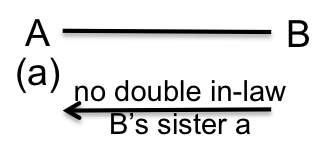
\includegraphics{figures/engagement/straight-sirhai}
\caption{Straight engagement--Sirhai
\label{figure:engage_1}}
\end{figure}

\begin{figure}
\center
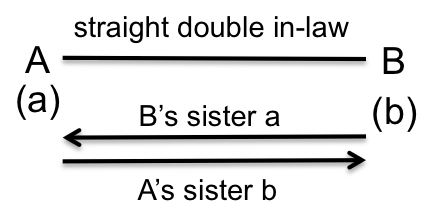
\includegraphics{figures/engagement/straight_opposite_2}
\caption{ Straight engagement Opposite double in-law
\label{figure:engage_2}}
\end{figure}

\begin{figure}
\center
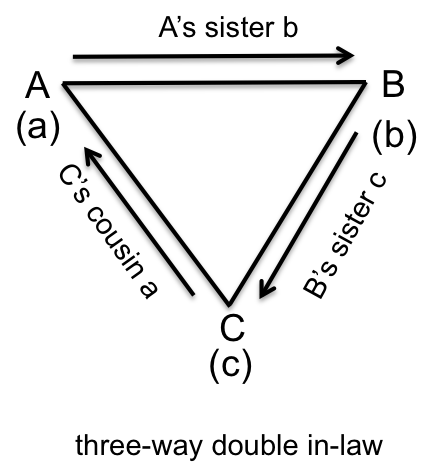
\includegraphics{figures/engagement/triple_3}
\caption{Three-way engagement
\label{figure:engage_3}}
\end{figure}

\begin{figure}
\center
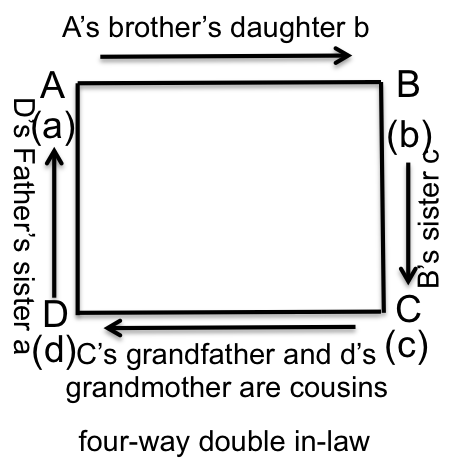
\includegraphics{figures/engagement/four_4}
\caption{Four-way engagement; note: C's grandfather and d's grandmother are cousins
\label{figure:engage_4}}
\end{figure}

\begin{figure}
\center
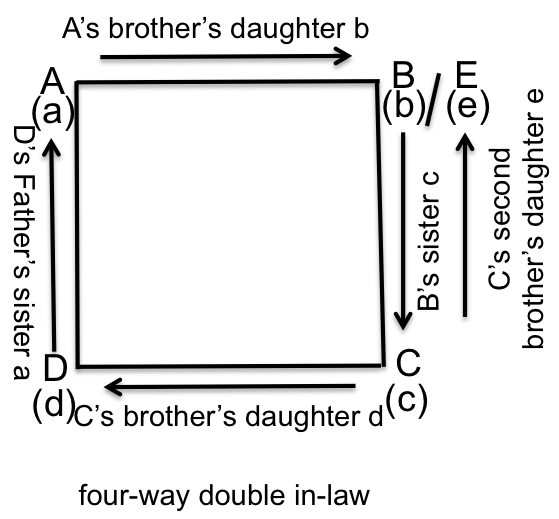
\includegraphics{figures/engagement/four_5}
\caption{Four-way engagement with two girl's offered in marriage; note1: In order to get C engaged, two girls, d and e were offered in marriage; note2: B and E are brothers
\label{figure:engage_5}}
\end{figure}

\begin{figure}
\center
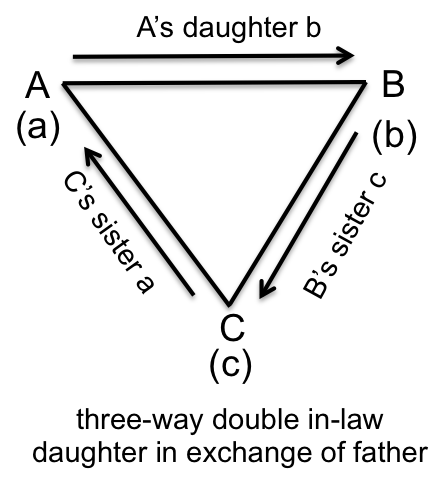
\includegraphics{figures/engagement/triple_6}
\caption{Three-way engagement; Daughter in exchange of father's engagement
\label{figure:engage_6}}
\end{figure}

\begin{figure}
\center
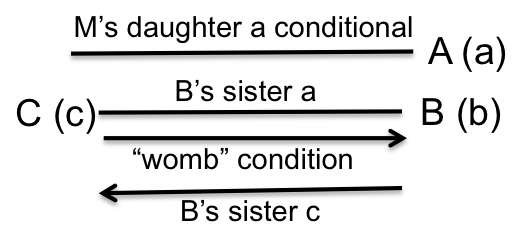
\includegraphics{figures/engagement/womb_7}
\caption{Womb written into marriage; M and N are brothers; a is daughter of M and C is son of N; M's daughter a is married to A and N has got womb written that the future daughter b of A(a) will be offered in exchange of his son C.
\label{figure:engage_7}}
\end{figure}

\begin{figure}
\center
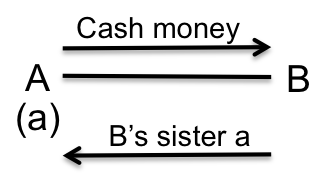
\includegraphics{figures/engagement/cash_8}
\caption{Engagement in exchange of cash money
\label{figure:engage_8}}
\end{figure}

Because of the system of double in-law, straight engagements happened
frequently. Such as a boy and a girl from one home marrying a girl and a boy
from the other. Such cases were possible when there is brother and sister on
both sides. When there are no sisters, distant relative was used as offering.
When there is a spare brother or sister, a third party was brought to use the
system. Sometimes, this happened with a fourth party too. This will be clear
with some diagrams and examples. The examples are taken from real marriages but
names are not given. Instead, alphabetical letters such as A, B, C are used.

In those days, three things were considered when looking for a bridegroom for a
girl: 1) Household--family, 2) Wealth, and 3) Boy. In household--family, the
social image and prosperity--wealth of the family was considered. There wasn't
much cash but it was considered if the family owns land, gold--silver and such
wealth. Further, the boy's profession--employment and his age was considered.

However, since the English education started in Thar and boys started to get
matriculation (around 1918-1919), the education became the most important
aspect to be considered when looking for the bridegroom for a girl. Different
situations demanded different considerations though.

In order to fix the engagement, bride's and bridegroom's parent did not meet with
each other but would use a third-party who is a trusty and known to both the
families. The discussion and conversation would go along for 6-8 months before
the declaration of engagement. If later on there are any disputes between the
two parties, a third party would intervene and addressed the issues. There was
no system of matching bride's and bridegroom's birth planets at the time of
engagement.

When town's elders get together for engagement, they would consider unmarried
boys and girls and set the two- three- or four-ways double in-laws and distant
relatives would communicate the conclusion to everyone involved. In those days
elders were respected and no one could over-ride their decisions. Once the
decision is made verbally, it was considered a fixed decision. Everyone had to
respect the decision.

Engagements were arranged such that the boy and girl could not meet each other.
There was no mutual interview or communication even after the engagement. There
were no photos which could be exchanged.

For the engagement ritual the holymen would be consulted for the right time and
main people of the community would get together at the girl's place. The
engagement was declared there and was registered in a ``\textbf{vahi}" or a
register. The names of both the parties and any double in-laws were registered.
If there is an agreement of a future offering, it was clearly registered so
that there is no dispute later on.

Girl's parents would offer a rupee coin and coconut to boy's parents which they
would accept. People joined from the bridegroom's family would identify people from
the family who are to be given the coin and coconut. Bridegroom's uncle or brother
would announce the names and bride's uncle or brother would bring rupee and
coconuts in a big pan and would go to each of them. The people the rupee and
coconut are offered would take them in lap or in a towel. First coconut was
offered to the paternal family and then to the maternal family. Afterwards the
brothers, cousins, son-in-laws and relatives were offered coconut. If someone
is not present and he is one of the person announced then someone else would
accept on his behalf. The intention of this ritual is to get each parties
introduced to the other parties. After this people would throw color on each
other, have milk and betelnuts and say good bye to each other.

On the other side, the women from the boys side would send milk to girl's
family. Bridegroom's sister-in-law or aunt would carry milk in a colored pot and
walk towards the bride's home. Other ladies from the relative's family would
join them. They would sing along while walking. Bride's family would gleefully
accept the milk. The milk was offered to the people of family and the empty
pots would be returned with small money. Bridegroom's family would bring dresses and
jewelry for the bride and gift it to them. Bridegroom's maternal and paternal uncle
would offer a ``\textbf{mud}" to bride's family. This included a full dress
which happened to be a sari, ghaghro and blouse and in jewellery, golden
head-ring, nose-ring and necklace were offered. In addition, silver anklets
were offered. This system was called \textbf{sakariyo}. After having meal at
bride's place, before leaving, they would offer one sari.

After the declaration of engagement, people from town would go to bridegroom's place
and would congratulate bridegroom's father. They would say ``\textbf{vadhai ahe,
vihan karyo}" meaning ``congratulations on the engagement". On which the father
would reply ``\textbf{thakur vadhaje}" meaning ``god's grace". Rupee coin and
coconut would be offered to people who came to congratulate. Wealthy families
of town or the families who had engagement after a long time would organize a
``\textbf{rihaan}" (party) at the house. Opium, betelnuts and cigarettes were
offered in these parties. Coconut and rupee were also offered. Bridegroom's relative
and family would sing songs which were called \textbf{raaso}. On the second,
third or fourth day, bridegroom's married sisters or aunts may also have
\textbf{raaso} at there place. Women joining in these singings would be offered
seven fresh dates. After the engagement and before the marriage, when there
were festivals such as \textbf{vadi teej}, \textbf{janmashtami},
\textbf{Diwali}, \textbf{Shivratri}, \textbf{Holi} etc., the bridegroom's family
would send sweets such as \textbf{sattu}, \textbf{pedha}, \textbf{gundpaak},
other sweets or dry fruits. Such a sending was called \textbf{bhaado moklyo}.

Engaged boy and girl would never visit their in-law's or in-law's relatives
places. They would not share a vehicle, a seat or would not sit together at a
meal on any social function. Bridegroom would not speak to the in-law's family
members. Bridegroom would never shake hands with his in-law's or any members of
in-law's family. Mother-in-law would never speak to her son-in-law and the
daughter-in-law would never speak to her male in-laws. This kind of decorum was
observed forever from the bride. If a girl is around and her would-be in-laws
appears, the girl would run away.

If a would-be mother-in-law wants to treat her would-be son-in-law, she would
invite her to a neighbor's house. Boy would be accompanied by his 2-4 friends
where the mother-in-law would offer milk to son-in-law and his friends. This
ritual was called ``\textbf{dudh piyaryo}". Everyone would have meal there.
Mother-in-law would offer coconut, handkerchief filled with goodies and dresses
etc. Son-in-law would also offer sweets to children and sister-in-law. 

Son-in-law was addressed with a special prefix or suffix: \textbf{``sahukar or
shah"}. For example if the name is Roopchand, he would be addressed as
Roopchand Shah. This way his respect was maintained.

If the engaged girl dies, the girl's parent would offer another girl or a
relative's girl in marriage so that the other marriages which are linked under
the double in-law system would not break. Sometimes wise people would not break
the marriage and would continue with the other marriages without any amends.

If the bridegroom dies after engagement, the girl would be engaged elsewhere.
Engagements done at a younger age would stay for a long  time, sometimes for
7-8 years. If the girl is too young or there are other obligations and marriage
dates are not fixed for a long time, both parties would understand such
situations and would normally not insist on a fixed date or period for the
wedding. The same understanding prevailed in the case of linked marriages under
the double in-law system. The saying was that \textbf{``vaal vichhaye dinha
ahin to sahe juno paise"} which roughly translates to an expression that if
hair is offered as carpet everything has to be considered.

Sometimes it so happened that a widower would have to be engaged with  the
girl. In the system of double in-law the aim was always bridegroom's marriage and
girl's choices were not given any priorities. Another thing is that if one's
own daughter gets in some trouble after marriage at the in-law's place then the
daughter-in-law was also treated badly to avenge this.

\section{Marriage}
In human life, birth and death are in the hands of almighty. Humans do not have
much control over them. While marriage is organized by the man himself and he
enjoys its bliss. This bliss happens only once in life. (Although man can marry
twice or thrice). Now let us see the old system prevalent in Maheshwari
community:

\paragraph{Fixing the date.} After engagement, when bride's and bridegroom's family
think of marriage, they would consult the holymen known to them. The holymen
would suggest 2 to 3 possible dates. Out of these, the date agreeable to both
parties would be fixed as marriage date. Some dates required that bridegroom or
bride needed to perform a special ritual which had to be agreeable to both
parties. Mostly people would select clean dates where no such rituals were
required. 

\paragraph{Writing Marriage.} Before the date of marriage, on an auspicious day,
bride's family would invite their relatives and 2-3 people from bridegroom's family.
At an auspicious time, everyone would gather at a temple or at bride's home.
The holyman would invite bride's father or brother for a ritual. He would wear a
red turban or an embroidered hat. After the ritual, the holyman would write a
marriage card on a blank paper. He would write the details of bride and bridegroom
and their parent's names, date marriage and planetary positions etc. He would
prepare a \textit{kundali} of the marriage. He would suggest if any additional
rituals are required. The marriage-card would be sprinkled with red kumkum
powder. \textit{Gaudhulik} wedding meaning the time when cows returned in dusk
and dust would fly was considered the best time for wedding or the night time.
Wedding were not organized during the daytime. Holyman would offer yellow rice
and would do a teeka to everyone present at the time of writing marriage. This
meant that the marriage was written in witness of everybody present. In the end
he would collect the yellow rice back from everyone, would add coin, betelnut,
7 dates, turmeric piece and put into the paper and wrap the paper. He would
make a Swastik on the paper and would write the bride's name on top. Rupee coin
and coconut would be offered to the people present from the bridegroom's side.
Children would get small money. People would disperse after having smoke and
betelnut. The marriage packet (\textbf{``pado"}) would not be put on floor. It
had to be put on chair or cot. Homes where marriages were written and their
relatives would not go to any funerals until the wedding is over.

\paragraph{Marriage ``sojhna".} Own relatives or neighbor's 4-5 married woman
would perform this ritual. They would put a kumkum swastik on a pan and put a
fistful of salt, rice, moong beans and juwar and would clean and separate them.
The bride would be seated on a cot and they would sing \textbf{``saahevero"}
songs. Afterwards the marriage packet would be tied again. This ritual was
called \textbf{``lagna sohya"}. The participating women would be offered dates.

\paragraph{Sending of Marriage.} The products of the above mentioned ``sojhna"
ritual were put in small cloth packets and would be sent to the bridegroom's family
via a gardener. Care would be taken that the marriage packet reaches the
bridegroom's place as soon as possible. Along with the marriage packet, girl's
father would write a letter in which he would write his family's name,
ancestry, salutations to bridegroom's family members and their relatives.
Afterwards, would mention that their daughter's auspicious wedding has been
written and the agreed upon date and would invite the bridegroom's family to come
with a \textbf{``surangi jaan"} or colorful procession to wed his daughter. If
the gardener had to go to another town, they would rent a camel for him. When
the gardener reaches the bridegroom's place, he would be welcomed with water and
salt crystals/nuggets. The marriage packet would be opened and a similar sojhna
ritual would be performed by 4-5 married woman with bridegroom seated on a cot. The
gardener would get 10-20 Rupees as gift and some cloth. He would be offered
meal and bridegroom's family would arrange for his travel back. Bridegroom's marriage has
arrived was soon known to people of the town and they would come to
congratulate bridegroom's family. Everyone was given coin and coconut. Some families
would organize a \textbf{rihan}.

\paragraph{Invitation Card.} After the marriage sojhna event, both parties would
write invitations to their relatives. The invitation cards were written by hand
and sprinkled with kumkum powder in those days. If close relatives are in a
different town then the invitation card would be given in person and
hand-to-hand. Sixteen jaggery \textbf{laddu} and 1 syrup \textbf{laddu} were
also given along with the invitation card. Others were sent invitation cards by
post. Care was taken as to see that no relative is forgotten. Close relatives
would take this opportunity to steal respect by taking offense and the hosts
would go above and beyond to coax them. Hosts would politely insist and say
\textbf{``maahnje otte te chadho"} meaning please come to my home. In extreme
cases bride's father would say, \textbf{``tahje page potiyo rakha to"} which
roughly translates to all my honor is at your feet.

\paragraph{Raw oil.} About ten days before the wedding, bridegroom/bride would be
seated on a cot at their home and they would be adorned with oil and songs
would be sung. In order to get the bridegroom up from the cot, his brother or uncle
would say, \textbf{``uthi tana bhalo uth deisa"} meaning, get up, will give you
a nice camel. Bride would also be got up from the cot by her brother or uncle
and she would get money or ring. At this time Bride/Bridegroom's leg would be tied
with \textbf{``laan"} which was a thread with some iron ring, sea-shell and
sealing wax. This was done so that they remain safe of foul play and bad
spirits. Such bride/bridegroom were called oil adorned and would not go out of home
much. Bridegroom would get back massage from a visiting barber everyday. Bride would
also get back massage from a female barber. A \textbf{``devakotho"} would be
painted on the northern wall of home in which Lord Ganesh, Sun-moon,
bride-bridegroom, bed-cushion etc. would be drawn. These were bordered with colorful
boundaries and would look beautiful. Girl's devakotho would have 2-4
riddles/puzzles written over it.

\paragraph{Nanani-Dadani.} Bride's maternal and paternal grand parents would
offer one day's meal to all the invited relatives. This was called
\textbf{``nanani-dadani"}.

\paragraph{Laapsi.} About five days before marriage, bridegroom's family will cook
\textbf{laapsi} and would distribute it to the community. Three people would go
door to door with a large beaker full of laapsi. Two would hold the beaker and
the third would measure 50 tolas (approx. 500 gram) of lapsi and give it to the
family. They would give more if there is any guest in the family at the time.

\paragraph{Vinyakh.} Two-three days before the day of wedding (\textbf{paarnet)},
the Vinyakh ritual would take place. Vinyakh means the worship of Lord Ganesh.
Bride/Bridegroom would sit in from on their devakotho on a cot. Songs similar to raw
oil ritual would be sung and all relatives would have meals at the hosts place.
On the right side of the devakotho, a cotton plug dipped in ghee would be
pushed against the wall seven times making seven streams of ghee from top to
bottom. This was called \textbf{maae uthiyarta} meaning remembering the seven
rivers. Bridegroom would wear a big golden necklace.  

\paragraph{Vinaho.} Two to four days before the wedding, family's relatives
would start arriving at the family's place. They would bring $1/2$ to 1 kilo of
sweets with them. This sweet was called \textbf{vinaho} and would get
distributed among the guests at the time of meals. Until the wedding sweets
such as \textit{magat} are made, the vinaho was used in meals. This way people
would know who has brought what. At the end of the marriage when sweets were
distributed to departing guests, the vinaho was taken into account.

\paragraph{Mogar.} In the home with marriage, the most used sweet was
\textbf{magat}. Rarely was seen a wedding without magat. To prepare magat, men
would be invited from among relatives. A brick furnace would be prepared in the
night. The mogar was made under the supervision of experienced and knowledgeable
person. This work was done through labor and community member's cooperation. In
a large deep pan the flour would be roasted. Two persons would stir the flour
with large six-feet long iron spoons. When they are tired, the next two people
would take their place. This way they would all take turns in the activity of
stirring the massive amount of flour. The roasted flour thus made was called
mogar. Adding sugar and ghee to mogar made \textbf{magat}. Everyone present
would eat the magat. Mogar thus made would not spoil for six more months and
magat would be ready in minutes. A detailed recipe for magat is given later.
(Such a process of preparing magat has not been heard of in any other
community).

\paragraph{Siloka.} On the night of Vinyakh, and thereafter, there would be
chanting of siloka (god's sloka) at bridegroom's place. 25-30 people would sit
together and one would start chanting slokas. 5-7 people would catch up the
tune enthusiastically. This was called \textbf{tuk jhalai}. People would have
betelnuts, sugar, cigarette, fennel and would leave.

\paragraph{Jaan.} Jaan or the marriage procession would go on feet if the
marriage is in the same town. If the marriage is in a different town, they
would hire camels. On the way they would take break and had magat and savoury
fried gram lentils for snack. Magat would be stored in brass pots. Care would
be taken as to who joins the procession. If someone who joins without a
relation then the hosts would say this is \textbf{lakho jaani} meaning a
freebie. When the jaan is about to reach town, the bride family people would go
out to receive jaan. Jaan would arrive one day before wedding. The day the jaan
arrives, they will get camels decorated with adornments and would ride camel
and make camel jump and dance. The bridegroom (\textbf{lado}) would wear soiled
clothes with massage oil and turmeric and a yellow turban so he would be
readily recognized. Lado would distribute money at the time of riding camel.
Elderly women and bridegroom's mother would not join the jaan.

\paragraph{Jaan-ro-dero.} The place where the jaan would lodge and board is
called \textbf{jaan-ro-dero}. There, for the convenience of jaan, bride family
would arrange bed, cushions, cots etc. Members of jaan would prepare food
themselves and would eat. Bride's family would send in some snacks. Relatives
of jaan members would send them curd.

\paragraph{Mandhotani.} Bride's family would order two festoons from town's
carpenter. It would be colored red. Festoon means three wooden strips joined in
a triangle where in the top two strips are decorated with two sparrows each
shaped wooden pieces and the top angled part is decorated with one sparrow
shaped wooden piece. Five sparrows symbolize five god-goddess:
\textbf{``Saraswati samru Sharda, Dhyavu dev Ganesh; paanch dev raksha karo,
Brahma, Vishnu, Mahesh"}. Bride's family would hang to the roof angle, a mud
plate, roti and raw \textit{papad}. Afterwards, the festoon would be tied to
the home's door. After that, they would be accompanied by a holyman and would
go to the jaan-ro-dero. A drummer would beat the drum in front. 5-7 children
would walk with mud plate, perforated wheat flour roti, sugar, cotton thread,
clay pots etc. Men would follow them. House's daughter-in-law would tie a
decorated head band and would carry a colored pot filled with milk. She would
be followed by other woman singing songs. After reaching at the jaan-ro-dero,
people would greet the jaan members and sit together with them. The woman with
milk would be welcomed with salt-water. Bridegroom would do \textbf{``bandai"} to the
milk pot by touching his turban's end cloth to the pot and then touching the
cloth to his face. He would do this 4-5 times. Holyman would tie the festoon to
the door and other things to the hook up the roof. Jaan members would greet
others with cigarette and betelnuts. After a while, they will return back.

\paragraph{Nani Kholo.} Bridegroom, Best Man and some friends would sing sloka, stop
frequently on the way and walk to the in-laws place. Best man would be usually
bridegroom's brother-in-law. Best man would carry a bag on his shoulder which had
coconuts and other useful things. In-laws would do the Nani Kholo ritual
meaning would offer a cloth-lungi to the bridegroom and gave coconuts.

\paragraph{Rihan.} It was a custom to organize \textbf{rihan} when the
procession came back to bridegroom's town. Bridegroom's father would ask for
permission for this. If there were two or three different processions in the
town it was discussed who gets to organize the rihan first. Families with
experience in organizing marriage processions, rihans and hosting
Mahajan-Maastaans were considered for this and accordingly order was set.

Town's gardener or two people from groom's side would start announcing rihan
aloud in the town and inviting people. This announcement is called
\textbf{``jaan-re-dere rihan ro sad"}. Opium was served as a custom in rihan.

\paragraph{Mandho.} Arrived groom's procession would organize a mandho in the
host's town meaning offer a meal. For this they would pay a nominal fees to
caste leaders and ask for a permission. The permission would be requested by
2-3 Dhuras in presence of Dhuras from bride's side. After getting the
permission, they would start by sending invitations to dhuras, close relatives
of the bride followed by other relatives in the town. Similarly, bride's guests
who have arrived from other towns (called \textbf{vachhat}) were also invited.
In meals \textit{siro} and \textit{khich} was prepared. Sometimes only khich
was prepared. Ghee would be poured in khich. Guests would bring their own
utensils, sides, water, pickles etc. and would have meal on the platforms
outside of houses. Mandho would normally be organized at the supper time.

\paragraph{Mahendi (henna).} Groom and bride and bride's friends would apply
henna over their palms on the night before the wedding.

\paragraph{Dhamoli.} Bride's elder relatives would observe a fast on the
wedding day so they would be offered meal with sweets the previous night.

\paragraph{Owaas (fast).} On the day of wedding, all the elderly relatives of
bride including parents, uncles and aunts, elder siblings would observe fast.
They would be offered fruits or cold drinks during the day time. Bride and
groom would not observe fast.

\paragraph{Vari.} The clothes and jewelry brought in by groom's party is called
\textbf{vari}. Jewelry offered at the time of engagement were brought back.
This jewelry was washed and offered again in many cases. Vari would include 15
to 20 \textbf{mu'd} (petticoat, top, chunar, etc.), 5 to 10 tolas (1 tola=11.66
grams) of golden jewelry, some silver jewelry and especially nose studs as they
were the sign of good fortune. Vari would be sent on a platter along with the
Lord Ganesha idol to bride's father on the day of the wedding. The vari was
taken by groom's uncle or elder brother to bride's place. A list on paper was
made of the items in the vari as follows:

Shri Ganesha Idol\\
Gold Jewelry (Name and weight of each item)\\
Silver Jewelry (Name and weight of each item)\\
Suitcase\\

The vari would be open as exhibition 4-5 days before the wedding and guests
would visit to see it. This exhibition was called \textbf{vari pathri}. Wedding
guests would also see the vari. The platter was returned to the groom's family
with some coin-money and coconut etc. Bride would wear the vari dresses at the
time of wedding.

Similarly, the things such as clothes and jewelry given to the bride by her
parents was called \textbf{de'j}. This was also put to exhibition 4-5 days
prior to wedding for visitors to see. This is called \textbf{de'j patharyo}.
Details about de'j is given later in this section.

\paragraph{Saho Paheran.} On the day of the wedding, the groom, the best man,
and friends would chant and go to groom's in-law's place. Their the brides
family would show the things in a platter put as \textbf{saho}. Groom would
get ``examined"~\textbf{purakhta} by his parents-in-law. Groom would stand
up on a small stool. A small claypot filled with coal and asafoetida was
put near door which the groom steps up on before entering the house. Before
that the holyman would take a yellow thread and would wrap it between the
large toe and ear 10-15 times to prepare a necklace which would be worn by
the groom's mother-in-law. This necklace is called \textbf{gebo}.
Mother-in-law would wear two wrapclothes. One was used to tie to the towel
of father-in-law (her husband). Then, mother-in-law would put the cloth
around groom's neck (\textbf{gano}) and would escort him into the house. Groom
would sit near the \textit{devakotho}. Their sisters-in-law would ask riddles
and puzzles written over the devakotho and if he couldn't solve they would
tease him by saying go ask your mother. Then, the things that groom brought
were weighed with a small balance brought in by the best man. Saho includes
\textbf{mod}, bedsheet sized loincloth, loincloth, Jodhpur's turban,
bush-shirt, coat, dhoti-cloth, and shoes embroidered with beads. Some
people would also include gold ring. Groom would wear new clothes on top of old
and would return. Groom would bath at a relative's home and the old clothes and
shoes (\textbf{kantarkhi}) would be given to the town barber. Similarly,
bride's old clothes were taken by barbette.

\paragraph{Choti Dhun.} 4-5 ladies from the bride's side would go to the place
where the groom has stayed and would wash his hair with oil-clay. They would
rub the clay on the back and give him a bath.

\paragraph{Beh Bandaan.} In order to decorate the wedding square 9 pots each
for the four corners (36 pots in total) would be ordered from town potter. The
pots were made in descending order in size so that the can stay on top of each
other. Out of these pots, bride's side ladies would carry 4-8 and take to the
groom for \textbf{bandaan} good wishes and take back to the wedding square.

\paragraph{Ghodi Chadhan.} The procession will start from groom's sister, aunt
or other married relative's place where the groom will ascend to a mare (male
horse was not used). A drummer would play drum. Sisters or other
relatives would do honoring ritual to mare. Groom would be given a towel to
wrap and a \textit{tilak} on forehead. Young sister, cousin or neice would sit
behind the groom on mare and would carry salt nuggets in a vessel and would
play it. That girl is called \textbf{loon ghori}. She would get special prize.
Then men would walk ahead of mare and women behind while singing songs. The
mare would be celebrated as it reaches bride's place. Girls would sprinkle raw
rice grains over the groom still seated on mare. Then everyone would go to the
groom's local relatives place where the groom would be wrapped with
\textit{lungi} or towel. After this groom and mare would proceed to
\textit{jaan-re-dere}. (These days Ghodi Chadhan is called varghodo which is
not appropriate. ``Varghodo" is much larger occassion whose details are
given separately.)

\paragraph{Purkhan.} About one hour before the time of wedding, the groom would
come to the in-law's place wearing the \textit{saho} dress, dagger in the
waistband, best man alongside and with other ladies. Here the parents-in-law
with the holyman would ritually ``examine" the groom. A plate with some sesame
seeds, sugar nuggets, wooden spoon, curds, wooden nails from the wedding square
were used for this ritual. Groom would stand over a stool near the gate.
Parents-in-law would touch seeds, wooden spoon to groom's chin, chest etc. as
per instructions given by the holyman. Mother-in-law would offer sugar nugget
to groom. Then groom would step down by stepping on the asafoetida and coal
filled claypot. Mother-in-law would pull groom's nose and put the \textit{gebo}
around groom's neck and escort him to the \textit{devakotha} (a square paper
pasted on wall with handmade drawings of dieties and other symbols).

\paragraph{Hathlevo.} On the day of the wedding, bride would stay at a
neighbor's or relatives place since morning. She wouldn't show face to her
parents. Bride was brought home just a short while before the groom arrives.
She would wear new dress and jewelry that has arrived as part of \textit{vari}.
Holyman would ask her to sit near the groom in front of the \textit{devakotha}.
Parents-in-law would wash groom's right big toe. Holyman would chant mantras
and would join right hands of bride and groom. They would place crushed
\textit{khejda} leaves between the palms. A handkerchief was tied over the
joined hands. Holyman would ask bride's father to say a few words about
\textit{kanyadaan} (a symbolic giving away the girl to the groom and his
family). Holyman would say the groom is like Lord Vishnu and bride is
like Goddess Laxmi. May they be couple for ever. They wouldn't say ``kanya
padhravo-saavdhan" etc. Holyman would tie thread over bride and groom's wrists.

\paragraph{Chori (wedding square).} After beh bandaan, four nails would be
nailed to raise the wedding square. Bride-groom would sit facing east in the
wedding square. They would typically sit over a small wooden stool (about 4-6
inches in height). Bride would sit on the right side of groom. Bride
would cover her face with double layers (\textbf{bitto ghunghat}) and would
hold the layers with her left hand. Best man would sit by the groom and a lady
who is bride's relative would sit by the bride. Holyman would sit in from of
bride-groom. Bride's parents would sit facing north. Some times, depending on
situation if bride's parent is not alive or around her uncle-aunt or elder
brother-sister-in-law would sit in place of parents. It was always remembered
who wedded the bride by sitting in the wedding square. Their part was always
similar to parents. Ladies would sing songs while the ladies on the groom's
side would sing mischevious songs (\textit{fatana}). Holyman would chant
mantras and would put offerings in the sacred fire lit in the middle of the
wedding square. Bride's parents would also throw offerings to the fire. If
there is any other ritual such as planetary worships, those were also performed
by the holyman at the time of wedding. All the leftovers from the wedding
ritual would be given to \textbf{varatiyas} (a caste). Just before the first
\textit{fera} (circling around the sacred fire) bride's younger brother would
stand by one corner of the wedding square holding rice in paper and would throw
the rice over bride-groom. This was called \textbf{hathda/taithiya dina}. This
was done for three feras. For the first three feras bride would lead the groom.
The direction would be from left to right. After each fera groom would sit on
the right and bride on the left. Just before the fourth fera groom's younger
brother would do taithiya. The bride was considered unmarried up to three feras
but after the fourth fera she would be considered married. At this time they
would sing \textbf{"chothe fere bai devar ri bhojai, dhian bai thi parayi"}
which roughly translate to--\textit{after the fourth fera the bride becomes her
brother-in-law's sister-in-law, and alien to her parents}. Bride's mother's
eyes would well up singing this. At the fourth fera the bride's in-laws
would put a saree over the bride and someone from the in-law's side would
come by the bride to ``take over".

\paragraph{Saptapadi.} After the feras the holyman would put seven betelnuts on
the ground and ask the bride and groom to stand nearby. He would touch bride's
toe with each betelnut and ask to take seven pledges. This is why it was called
\textit{saptapadi} meaning seven pledges. Just as a river leaves behind it's shape,
color and form and meets the sea, a woman leaves behind her whole
existance and meets her man. Just as sugar in the milk dissolves and
makes it sweet, woman mixes in a man's life and makes it sweet.

Marriage is a vow between a man and a woman to live together forever. The
\textit{saptapadi} is a symbol of such a long-lived togetherness. (It is really
worth understanding the meaning of the seven pledges in sanskrit spoken
by the holyman). The meaning of marriage is summarized in
table~\ref{tbl:marriage}. After the \textit{saptapadi} the holyman would ask the couple to see the North Pole Star.

\begin{table}[h]
\begin{center}
% use packages: array
\begin{tabular}{p{2.5cm}p{2.5cm}}
M & Merging \\
A & Ambition \\
R & Respect \\
R & Response \\
I & Intimacy \\
A & Accredition \\
G & Gaiety \\
E & Eternity \\
\end{tabular}
\end{center}
\caption{Meaning of marriage}
\label{tbl:marriage}
\end{table}

\paragraph{Kataari.} After the \textit{saptapadi} is over, the groom hands over
the kataari (dagger) to bride's brother and cousin who takes it to groom's
father at \textit{jaan-re-dere} and congratulates him with the words:
\textbf{vadhai aahe, avhaanjo dikro sukhsi parne utaryo ahe. karpanu karanla
halo.} which roughly translates to \textit{congratulations! your son has
wedded nicely and please come over for blessings.}. Both boys would
receive some money and return. 

\paragraph{Karpanu.} \textit{Karpanu} was done by groom's father first. The
money was given to the clan's holyman. After that bride's grandparents,
parents, and other relatives would do \textit{karpanu}. Water, milk,
\textit{gulaal} and a coin was put in a big copper platter. The person
doing \textit{karpanu} would take the coin and water in their palm and
would say what/how much they are doing as \textit{karpanu}. Husband and
wife would do karpanu together. After this the groom would \textbf{chori
varsaito} meaning would give away money and sweet dates by throwing
them around. All corners of the wedding square were tied across with
a thread and a sari was put in the middle. Groom's family would put
this sari. Housemaid would take that sari away.

\paragraph{Shoe Hiding.} Groom's sisters-in-law (bride's sisters) would hide
groom's shoes as a mischief. They would return the shoes only when their newly
wed brother-in-law (groom) gives them some money as \textit{laago}. 

\paragraph{Reflection in Ghee.} At the conclusion of karpanu the holyman would
untie the \textbf{hathlevo} off bride and groom's hands. Groom would have meal
with his brother-in-law and friends. The meal consisted of \textit{siro} and
\textit{puri}. Bride would sit at home where the fasting elders would see her
reflection in \textit{ghee} (clarified butter) in turns and blessed her. (this
custom might have started because married girl might be hesitant in
looking at elders directly). After this all would break fast and have
meals.

\paragraph{Jaan Vadhani.}

\paragraph{Anhura.} In the morning the bride would return to her parent's place
and would bring her friend's and small children along back to her in-law's
place to have meal for the first time. This was called \textbf{anhura jiman
aaya} which roughly translates to: \textit{anhura arrived for meal}. After
this, bride would return again to her parent's place.

\paragraph{Var Kalevo.} In the noon groom's father would offer meal to the
groom's procession members. This was called \textbf{var kalevo}. The meal
consisted of \textit{magat} (a sweet dish) and \textit{khich} (porridge).
Additional ghee would be added to this magat and it was called \textbf{kino
magat} (dirty magat). In the old times \textit{var kalevo} was done by
serving wheat flour flatbread weighing 1 to 1 $1\over2$ kilogram fried in
ghee.

\paragraph{Ring Game.} At the time of \textit{var kaleva} bride and groom would
sit near the \textit{devakotho}. In a platter, 27 raisins, 27 almonds (from
apricot kernel), 27 pennies, 29 sea-shells and groom's ring would be
put in water, gulaal and milk. The couple would try to fish out the ring with
their right hands. It was said the one who finds the ring would dominate the
household.

\paragraph{Tunk.} The official meals from bride's side to their in-laws would
begin on the third day. The guests would spend a month (later 10 to 15 days) at
the bride's place. Lunch meal would be provided by the bride's family while the
dinner they would arrange on their own. First such meal was called
\textbf{praan pat ro dhamu}. In such meals unless someone from the groom side
doesn't show up to eat the dish would stay put. Nobody would eat. Sometimes
such wait would last hours. If there were any grudges with groom's father these
were the chances to get apologies from him. Both the hosts (bride's side) and
the guests (groom's side) would sit together for meals. Up to 6 to 8 people
would eat together out of one plate. Someone from the bride's side would start
the meal by offering sweets to guests by putting a piece in their mouth by
hand. This would be followed by everyone offering sweets to each other in such
a way. Nobody's offering was rejected. Nobody would take the main course as
long as at least one plate is still having sweets. After finishing sweets
plates would be changed and \textit{khich} (porridge) was served. A pot full of
ghee was poured over khich or was offered with khich. Bride's family would also
invite some people from town to such meals. This was called \textbf{bhaktanu}.
In earlier days many people from the community would offer small money (between
1 to 25 paisa) in \textit{karpanu}. Anyone offering below 25 paise was
not invited for \textit{bhaktanu}. Before meals one plate was set aside for the
ancestors which was called \textbf{aalthaal}.

Sweets in \textit{tunk} included mostly \textit{magat} but sometimes
\textit{bundi}, \textit{mohanthaal}, \textit{jalebi} etc was also offered.

\paragraph{Kankan Chhodan.} The night after the wedding night was considered
the night of religion. Just before the third night the \textit{kankans} of the
couple was untied. The couple would meet for the first time that night and
begin the married life. This night was called \textbf{sohag-ri-raat}. Bride
would go to her in-laws during the day but would stay with her family in the
night. Son-in-law would visit her there and would stay overnight. If both
families are in the same town then the son-in-law would visit the in-laws for
meals and overnight stay for months.The custom was in place so that the married
woman would be less hesitant. 

\paragraph{Kalasho.}

\paragraph{Barothi.}

\paragraph{De`j.}

\paragraph{Handing Over.}

\paragraph{Rabroto.}

\paragraph{Parbat/Patti.}

\paragraph{Ghor.}

\paragraph{Moklani.}

\paragraph{Ravangi.}

\paragraph{Jaan Vadhani.}

\paragraph{Kumkum Pagla.}

\paragraph{Muh Joani.}

\paragraph{Dhobo Bharano.}

\paragraph{Tedo.}
\par
\begin{center}\framebox[1.1\width]{Special Note} \par\end{center}

\begin{center}\framebox[1.1\width]{Miscellaneous Notes} \par\end{center}

\section{Death} 
One's birth can be predicted 7-8 months in advance but death is unpredictable.
Nobody knows when death will happen unless some one inflicts it upon self
(commits suicide), which is a sin religiously and a social and legal crime. If
he gets lucky to live, he becomes unlucky to get punished by law.

Now let us see the prevalent traditions for deaths in the Maheshwari community:
When a person falls ill and has left all hopes of living, at that time a lamp
(with ghee as fuel) is lighted which is called \textbf{jivat divo}. The person
is taken down from the bed. The oldest son would put the person's head on his
lap which was called \text{godo dinho}. Geeta book was read for the dying so
that they can listen to something good. Relatives would declare the donations
they would make in the dying person's name such as grains, milk, ghee, curd,
utensils, grains for birds, animals etc. They would also declare how many
\textit{agiyarash} fast would they observe in the name of the dying. At this
last time family would send ghee and rice to local temple.

Sacred water of river Ganga, basil seeds, and curd is put in the dying person's
mouth. It is said that every form of life gets milk but not curd. Only human
\textit{yoni} gets to taste and enjoy curd. ( It was believed that the dying
person might not get curd in the next birth. ) A tiny gold grain (\textbf{tus})
was put in an eye. Someone experience would hold the pulse to learn and verify
death.

At the time of last hiccup before last breathe, water was poured over mouth
from a steel pot (\textbf{gagar}). This was called \textbf{paani thyo}. This
was considered very important event. If  this did not happen it was considered
that the dying person's soul went wrong way and the sons of the person were
criticized such as \textbf{moena lap panie kon thyo}. (This tradition was in
place so that the ill person is continuously taken care of and nobody stays
careless. When the breathe stops gets known timely.) At the time of pouring
water everyone would cry loudly so that neighbours would know someone has died.

Dead body's hands and legs would be straightened and the body would be laid
such that the head stays in the North direction. Ear and Nose were plugged with
cotton plugs. Eyes were closed. A brick was placed under their head.

After that in one corner of the room a square was made with cowdung
(\textbf{dhor deita}). The body was washed/bathed, wrapped in a fresh white
cloth and laid down on the square. Forehead was spotted with \textit{Tilaka}.
For the shroud (\textbf{kafan}), a \textbf{nav nali} ( approximately 36 square
feet ). The shroud would be wrapped and sewed on one side and about 1 feet
extra was left open on the other side. This shroud was wrapped on the body with
the open part on the head side. Three small silk cushions were made with cotton
filling.

The funeral procession would start by placing the body on a \textit{nanami} made
of two vertical bamboo sticks and seven horizontal wooden plates tied between
them with jute ropes. Dried grass, dried plant of basil and a small piece of
sandalwood was put on top of nanami. If an unmarried boy has passed away, a
lungi cloth would put as shroud. If a married young man has passed away then
his wife's saree is draped as shroud. Dying married man would be given lungi
from in-laws home called \textbf{ochhado} and if the dying person is a young
married woman, she would be given a pair of clothes (\textit{madd}) from her
in-laws home. If the dying person is an old lady, a necklace made up of basil
wood beads would be put in her neck. Often for the elderly people silken satin
cloth would be used as shroud. The body is tied to the nanami with a sacred
thread and some \textit{gulaal} is sprayed. Dying man's widow would break her
bangles and remove the nose stud. (These were considered the signs of a married
woman.)

Relatives living far away were sent telegrams. However, it took some time for
the telegram to reach and relatives to come so they were not waited for. As
much as possible the funeral procession would start immediately. They would not
let the body stay overnight. However, funerals were never held in night. In the
times of poor communications and transportation, the dying person was given
last rites in the same town where he died.

Before the procession, the relatives of the dead would circumnavigate the
nanami and pray for the departed soul's piece. Barbers were called to home to
shave off hair, beard, moustache etc. of the brothers and sons of the dead. If
someone does not want to clean shave head then the sideburns were shaved and
was said to have \textbf{sirbadra dinha}. This was an indication that someone
in the family has died. Relatives would also put coconuts near the body which
was taken with the funeral.

Townsman would reach the cremation ground with a \textbf{kumbhat} wood load on
his camel. This wood would weigh about 100-140 Kilogram. Family's daughters in
law would clean the floor from the place the body is put to the street outside
the home. They would use their saree to dust the floor. This was called
\textbf{vehdo boharyo}.

To give shoulder to the nanami, first great grandson then grandson, son,
brother, daughter's son etc. would be the order. If the dying person has great
grandson, it was said he has a golden stairs to heaven meaning he has lived a
happy and fulfilling life. Nanami was lifted such that head remains on the
front. Two people in the front and two in the back, when they lift the nanami,
everyone would cry loudly. Nanami would leave from the main door of home. There
have been instances where daughter's marriage ceremony is about to take place
and father dies. In such cases nanami is taken out from the back of the house,
in some cases after breaking the court wall of house. Dying person's elder
relatives such as father, uncle, elder brother etc. would not join the
procession to crematorium grounds. Husband would also not join the cremation
procession of his wife. Women would also not go. However, women would go to
some distance in elderly person's procession chanting religious songs
(\textbf{bhajans}) and return back. At the time of procession to crematorium
grounds, household and neighbourhood women would cry which is called
\textbf{munhda odhti}. 

During procession, three balls of wheat were made. First was given to dog/cow
at the time of beginning the procession, second at the time of reaching
(\textbf{vesahi taane}) and third at the time of cremation.

If death has occurred during some special time of calendar year such as
\textit{panchak} five such wheat floor balls were taken. It was said that a
dying person during the time of panchak would cause death of five more people
from the community. To avoid this, five wheat balls were made. Other people
would take some grains tied in towels and would give those grains to birds at
the crematorial grounds. They would wrap the towel in their necks. One person
would chant \textit{``raam naam satya hai"} from behind the procession which was
repeated in chorus by others. They would chant this all the way. Dying person's
relatives would change shoulders among themselves. Relatives would throw sugar
\textit{patashas} and coins during the procession.

A little before the crematorial grounds, at a decided spot, after sprinkling
some water on the ground, the nanami would be brought down to the ground. The
end of the cloth shroud would be torn and tied to a tree. The nanami would then
be turned. Now the original people who lifted the nanami in the beginning of the
procession would come back to the nanami and it would enter the crematorial
grounds.

At the crematorial ground, after pouring some water and grains, nanami was put
on floor. A place where there is no recent cremation, wood is arranged after
putting a coin and some water sprinkles. Some dried grass was put on top. Then,
the body was put on top with head to the North direction. Ghee was applied on
body's hands, legs, forehead etc. Then after putting more wood on top the pyre
was completed. Some coconuts were also put in between.

Initially, all four people who gave shoulders or the eldest son would
circumnavigate the pyre and would put fire to the right toe of the body.
Everybody would sit at a distance. 2-3 experienced people would inspect the
pyre frequently. They would turn the wood or if required added more ghee and
wood. Special care was taken so as no part of the body is left unburnt. Such
parts were brain and women's waist. After the pyre is burnt fully, people would
return after bowing to the pyre.

These cremators would go straight to the village well where their children
would be waiting for them with fresh clothes. They would take bath in the same
clothes as they are wearing and then change into fresh clothes. If one has to
bath at home then they would go to the dead person's home. One person who has
already been taken bath would bring some water from inside the house and put
some on each of the cremators head. After this, other than family members, all
would disperse. As cremators come back near home, they would cry. Cremators
from the family would bath at home with clothes on and then would change into
fresh clothes. Died person's son would go to his mother and console her. Roti
was offered to cow and dog and grains to birds.

Meanwhile meals get cooked at home or at the neighbour's. If the died person is
young then pearl millet (\textbf{bajra}) roti and rabdi/moong dal was cooked
and of the died person is elderly then wheat \textit{tikli} (a type of roti)
and dal was cooked.

Everyone would have meals together so that the close family members would also
eat something and would not feel too sad. Until the 11th day at home everybody
would observe \textbf{sutak}, meaning nobody would go to temple and nobody
would do any worshipping at home. 

In third day, \textbf{teiyo} was observed. At this time, relatives in the town
were asked to wash their heads. Everyone would get together and with a
\textit{maharaj}, 2-3 people would go to the crematorium. Others would go to
the well. A water container and some milk would be sent in advance to the
crematorium with which the pyre would be cooled down. This was called
\textbf{chita tharta}. Bones were collected from the pyre and take them to the
well. There, near a peepal (sacred fig) tree the late person would be given
last rites. First the son and then brother etc. would take some water, milk and
leaf and pour some water from hand (108 times) on the ossified bone put on top
of a wheat flour ball. Those who have worn janoi (sacred thread) would do the
same with the thread held between thumb and small finger. After this, they
would put fuller's earth (\textbf{mait, multani mati}) in head and wash it with
water and return home. The ossified bones would be wrapped in a silk piece of
cloth. Alongside \textit{panchratna}(five metals-gold, silver, iron, copper and
brass) and honey would be put and this all would be wrapped in deer skin. Some
fuller's earth would be applied on top and then this would put in a box. This
box was not put on floor but in cupboard or some shelf.

If no lamp has lit then after washing head on teiya, they would lit a ghee
lamp. Died person's son or grandson would take care of the lamp which was
called \textbf{dive betho}. He was given everything to eat that he wished for
such as sweets etc. It was believed that these things will reach the died
person. The lamp was kept alight continuously. 

This boy would offer rites everyday with water, milk, leaf and wheat flour ball
with 108 times water pouring using both palms near the peepal tree. Alongside,
another person would carry water in a bucket and a metal pot. After the day of
death, each day the flour balls would be increased which became 11 at the
eleventh day. After the rites, the ball was given to cow which was called the
\textbf{bahar-ri-kriya} ritual.

On the day of teiya, died person's in-laws would offer rice and ghee which was
called \textbf{ras dino}. On that day other relatives would wear turbans. Close
relatives would tie some cloth on head until 11th day. Sons and brothers would
not wear shirt. On that day a holy person or priest (\textbf{maharaj}) would
start reading \textbf{garudpuran} which was listened by the women of the
family. 

If the died person is elderly, then the in-laws of their sons would come with
color and would offer a rupee coin and coconut.

On the day of teiya distant relatives were written letters which included the
news of the death and the date of death and dates of 11th and 12th day. Right
corner of the postcard was torn off so that the receivers would know the letter
is about death news.

In the evening of teiya, in a lid of earthen pot, sweets, food and opium etc.
(things liked by the departed soul) with an iron tong and water would be taken
to crematorium. In a street by the crematorium, the lid would be put on floor
and the water would be poured around. The iron tong was taken along so as to
avoid some evil spirit talking the food away.

Men would sit at the home of the departed sould for 12 days. They would spread
sheets etc. (\textbf{tapad vichhaye}) and sit on it. People from town or other
towns would arrive to console the family. They were offered cigarettes,
betelnuts and opium. Women would fold double the end of their saree and put on
their head so that they can put the saree over their face and cry
(\textbf{ochhingar}) when they see some relative coming to console them. This
type of doubled folded saree would also serve as a sign that the woman has
someone passed away in the family.

Household's oldest daughter-in-law, married daughter, or maternal and paternal
aunt's were the main women sitting in mourning. Younger women would do chores.
When some other women come to console, they would also join in mourning.
Depending on the departed soul's age, situation, they would sing mourning songs
(dirges). Visiting women would join in mourning for some time then would pull
the saree over the head of the host woman and would console her to calm down
(\textbf{maat karaiti}). Women of house and visiting women would not wear
\textit{bindi} on forehead. This ritual would continue for months.

Relatives living in other towns, as and when they come to know of the
departure, they would inform others in the town about the death and would say
\textbf{paani ro kahije ta} which would mean that others will come to their
home to console. The relatives would do the water rite 108 times as mentioned
above. They would also sprinkle water over the gathered people and then
disperse. Women would mourn similar to women of the departed person's household
by double folding saree and putting it over their face.

After teiya, the departed's relatives would eat at their house. The relatives
would sleep on floor on a sheet without mattress (\textbf{ukhrade}).

On the midnight of the tenth day the lamp would be taken by the boy to a place
with crossroads \textbf{vathan} or \textbf{chovate}. He would dig a small pit
and store the lamp there. He would sprinkle some water. Person taking this lamp
would not speak and would not look back.

Closer relatives from other towns would come on 11th day to visit called
\textbf{kaanehaar} while distant relatives would come on 12th day. If the
visitor is a close relative, he would put a cloth on his head as he comes close
to home and would start crying aloud while coming to the home with wailing
sounds like \textit{ohh my uncle} (\textbf{he mahnja kaka}) or brother or any
other name depending on the relation. This way it would be known who is the
person. Visiting women relatives would also cry like this. Visitor would sit
near the door where someone from house would come and give water. After
drinking water, wherever the mourning is happening, he would sit on the corner
for sometime and then would get up and go to the main person and would console
him by hugging. This is called \textbf{sampharto}. Or, he would shake hand and
say kind words, eg. \textit{ram-ram} and ask about wellness. Similarly, he
would say \textit{ram-ram} to other people around and would sit down.

Visiting woman on \textbf{kaanehaar} would also \textbf{sampharti} to host
women, elderly men etc. depending upon relationship. Such mourning would go on
continuously.

Priest or holyman would assist the son of the departed in 11th day rituals.
They would sit near the sacred firepit, would chant mantras and do rituals so
that the departed soul could rest in piece. They would add grains-sesame-ghee
to the sacred firepit. They would add sutak to the fire. This was called
\textbf{ote-ri-kriya}. In memory of the departed, who would do what kind of
donations and fasts, that would also be declared. In the 11th day meal, they
would cook sugar \textit{halwa} and close relatives would eat together. After
things get burnt in the sacred firepit, the priest or holyman would also have
meals.

Priest would help tie turban (\textbf{potia ra var deraita}). For this
ceremony, people from community would be invited. Priest would do a tilak on
forehead and would give basil leaves to them. This ceremony would mark end of
mourning. However, in reality, some kind of mourning would continue for 8-12
months.

In-laws would put on shirts over the mourning hosts. Father-in-law would offer
money to their son-in-law. Visiting daughter and her \textbf{vejada} (children)
would get clothes and sweets. If the departed soul is a parent of a married
woman, she would also get some gold jewelry. Visiting people would give money
to departed's widow which was called \textbf{thigdi ra paisa}.

If possible, the departed's son, nephew or brother would carry the ossified
bones to Pushkar or Haridwar. They would put the ossified bones in bag/suitcase
and hold a wooden stick with them. Before leaving they would call the departed
by relation or name eg. father/mother/uncle come with me (\textbf {mi bheda
halo}). He would not look back and would not speak. On the way when he would
dine, sit or sleep, he would ask the departed's soul to sit, sleep, eat etc.
After reaching, he would do the appropriate ritual with the help of local
holyman, offer meals to the holymen and appropriate donation for the rituals.
This ritual was called \textbf{taravto} meaning letting the departed soul's
ossified bones be merge into the holy waters. He would also register his name
on the registries maintained by the local holymen. After this ritual, he would
let his head shave there. He would return after finishing everything.

If no one is able to go to Haridwar or Pushkar for this ritual, the box with
ossified bones would be sent by post or parcel to the holyman and they would
themselves do the rituals. The donation for holyman would be sent via
money order. Such holyman would visit Thar's villages once every 4-5 years and
would obtain some money as donation.

On the 12th day, the departed's son would go to \textit{dhura} (a division of
community), would wear towel around neck and would request \textbf{assanje
vadil ri osser ri mokal dyo} meaning grant permission to organize a community
feast in memory of the departed soul. For this there was a special saying as
\textbf{muth ghughariya ri karan do}. Depending on the past deeds by the family
on other similar occasions, the dhura would accordingly grant permission.

A community rihan is organized on 12th day where opium was used. After that, in
sweets \textit{dahithara} (a sweet made up of curd)/\textit{jalebi} (a sweet
made up of fermented flour, oil/ghee and syrup)/\textit{bundi} (a sweet made up
of chick peas floor, ghee and sugar) (in increasing order) would be cooked
depending on one's status and position. If some likes to do \textbf{panch
pakwan} they would cook five sweets as \textit{bundi}, \textit{jalebi},
\textit{dohti}(a sweet made up of flour, ghee, sugar), \textit{mesu},
\textit{mohanthal}(a sweet made up of chick peas flour, milk, sugar, ghee).
Brahmins were said to have done Brahmbhoj. Each Brahmin with sacred thread
would be offered a donation of a rupee or more.

Arriving Brahmin would have meal for himself and would take a fixed amount of
sweet per family member at the time of leaving. This is called \textbf{biro}.

Dhura's guests arriving for feast would bring their own utensils, cold water,
poppadams, pickles etc. Feast would happen in the street where everyone would
eat together.

Such community feast was called \textbf{mahajan} and when done by Brahmins, it
was called \textbf{maastaan}. If someone organizes this kind of feast in memory
of their departed elders then it was said that one has done
\textbf{mahajan-maastaan} and this would get registered in community holyman's
registers.

Maheshwaris would spend a significant amount of money in such \textbf{ossers}.
For poor people, this would mean that all their savings would get washed off
and they might have to take loans to organize such events.

In memory of the departed, priest would read \textit{Garud Puran} from teiya
till 13th day. It would end on 13th day.

People who have visited in kaanehaar would also offer some donations to the
priest reading the Garud Puran which was noted in a notebook(\textbf{bandi}).
Additionally, family would give cot, duvets, beddings, cushions, mattress,
light, cow etc. in donation. Instead of real cow, a symbolic token of small
silver cow would be given which was said to help the departed reach heaven. It
was said that the departed would hold the tail of this cow and swim across the
Vaiterni river and would reach heaven.

After the 12th day, almost everyone would disperse, only close relatives would
stay. On 17th or 18th day \textbf{Maasi chhant} (monthly ritual) would be done
when the priest would be offered meal and a donation. After this everyone would
leave. Six monthly and annual ritual would be respectively done on 5th and 11th
month during the waning (\textbf{vad}) part of the lunar calendar. Family
members would be invited for six monthly and annual rituals by writing letters.
Brahmin would do sacred fire-pit ritual and would obtain a donation.

After the departed's death date, one \textbf{shraaddhs paksh} would be left and
in the next \textbf{shraddh paksh}, their first \textbf{shraddh} would be
observed. At this time all the relatives would be informed by postal letters.
Sweets such as \textbf{kheer} (a kind of rice pudding) and
\textbf{muthia-ra-laddu} (a sweet made up of flour and ghee) would be made.
Alongside wheat floor \textbf{tikli} (a kind of roti) and
\textbf{chibhde-karing-guvar fali ro saag} (mixed melons vegetables) would be
cooked. More than one brahmins would be invited for meals. After that, on each
of the Shraaddhs, only family members, a brahmin and daughters would be invited
for meals.

Widow would not step out of house until after the first Shraaddh of the
departed which was called \textbf{khuno paadyo}. Such a thing would sometimes
happen for two years (if a person is dies just after the Shraaddh paksh, his
Shraaddh would be observed after two years). After first Shraaddh, woman's
parents would take her to their home and would offer her a new pair of clothes.
This was called \textbf{khuno chhadayo}(she can step out the door now). 

\paragraph{Vaikunthi.} If the departed is a leading person in the community and
of upper status then their children would celebrate a vaikunthi for them. For
this, the corpse would be bathed and arranged such that it is sitting upright
with straight neck. 

A wooden chariot would be made with three sides open and the back side closed.
The departed would be seated straight on this chariot. The chariot would be
decorated and there will be four handles around it which would be lifted by
four turbanated people. Red color powder (gulaal) would be sprinkled all over
during the procession. Also, money and sugar candies (\textbf{patasha}) would
be distributed along way.

Temples on the way or all temples in the town were visited and the procession
would stop for a short while. The pyre would be set with the body straight in
seated position and wood etc. would be arranged around it. Before doing
Vaikunthi, a permission was sought from the community and the community will
consider all the relevant factors and past of the family before making
appropriate decision.

The meals would include panch-pakwan. Mahajan-Maastaan would be offered meal.
Brahmins would get good donations.

After the formation of Pakistan, in Mithim Ranchhod-das Bekhatmal Dhirani and
his brothers celebrated Vaikunthi of their father, Mr. Bekhatmal. This
Vaikunthi was celebrated on 24/03/1982 which was probably the last in Thar.
Then, the departed's sons offered meals to the whole town of Mithi (including
community and non-community people such as muslims). In other towns of Thar
where Maheshwaris lived, they sent special people to cook sweets the same day
and distribute to Maheshwari households.

\paragraph{Infant or Child Death.} If an infant or a child is died because of
diseases such as Pox then they would be buried instead of cremation. After
wrapping them in appropriate shroud, digging a pit and the child would be
rested in there. Some salt would be sprinkled over the body so that it gets
dissolved in soil faster. Some thorns would be spread on top and then the pit
would be covered with soil. Thorns were put so that some animal may not dig the
pit and disturb the body.

\textbf{Note:} Elderly person, if passes away, it was called \textbf{``Ram
karyo"} and if a child passes, it was called \textbf{``pachho thayo"} meaning
``returned back".

\paragraph{Dirges.}
Dirges are called ``par" in Dhati. Women sing them while mourning behind a
person who passes away. Such dirges were sung about the person's life, their
age, the family they left behind etc. Even after trying no woman (or man) was
ready to sing these dirges, so they were not recorded here.

Widowed woman would normally sing dirges behind their husbands like so:\\
\textbf{hey hu to muthi} (became widow)\\
\textbf{hey mahnja bachiya na role gayo} (left my children alone)\\
etc.


\chapter{Religious Culture}
Religion links soul to the supreme. Religion connects the world with the
creator. Religion shows the way to rendezvous with the God.

There are many religions in this world and people observe their religion. Hindu
religion is the religion of Hindus. It is the oldest religion of all--it is a
\textit{sanatan} (eternal) religion and is also known as a vedic religion.

Thar Maheshwaris are Hindus and followed the Hindu religion. Maheshwari
community originated from the God Mahesh. So, Lord Shiwa was worshipped but
Maheshwaris were Vaishnavs. Every town had a temple. Temple is a leading symbol
of our culture and heritage. Eternal religion is incomplete without temples.
Temples are so integrated in Indian life that it is hard to believe any Indian
has not visited one in his/her lifetime. Many \textit{Murlidhar} temples were
built by Maheshwaris. Beautiful marble idols were brought from Jaipur and were
installed in temples. Shri Ganesh and Hanuman idols would also have a place in
such temples. Towns had \textit{Mataji} temples and \textit{Madhi} where people
would go for worship during \textit{Navratri} fastivities. Other Matajis such
as \textit{Sheetala Mata} idols would also be present in such temples.
\textit{Bhojaks} would maintain and take care of temples and were called
\textit{sevaks}. They would take care of temple's cleanliness, God's bathing,
decoration of the idol, prayers etc. Occasionally, people would donate gold and
silver which was taken care of by the sevaks. Musical instruments such as
drums, hand-symbals etc. would also be found in temples. These were used
occasionally during devotional songs and during festivities such as Holi.

There was not much literacy among Maheshwaris in Thar but there was tremendous
belief in almighty. Sanskrit knowledge was negligible but because of Gujarati
knowledge, people used to read Ramayana, Mahabharat, Bhagvadgita and Bhagvat.
Other religious text were also read. Such Gujarati books were mostly published
by the Akhand Anand Publishers in Ahmedabad city of Gujarat. When people
visited Gujarat for business, they would bring these books with them back home.

Women would visit temple almost everyday. They would donate some grains and
money. They offered 16 \textit{Akshats} (unbroken rice grains) and milk to
\textit{Shivalinga}. After bowing to the god in temple, they would hold a small
mirror put in temple towards god and then towards themselves. From a small bowl
of \textit{tilak}, they would dip a small stick and do a tilak on their
forehead to the tip of their nose. They would circumnavigate the temple. They
would chant devotional songs there. On special festivals such as
\textit{panthevari}, \textit{Holi}, \textit{Janmashtami}, \textit{Shivratri},
etc. related devotional songs would be chanted by community and towns people.

Every 11th and full moon day of the month, woman and some men would observe
fasts. On full moon day meals were taken after seeing and worshipping the moon.
\textit{Ganesh Chaturthi}, \textit{Hanuman Jayanti}, Mondays and Saturdays were
also observed as fasts by some people.

Towns will always have organization of religious stories called \textbf{katha}
in the evening. Usually, elderly women would go to listen to kathas. If there
is a touring playgroup for \textit{ramleela}, men-women would visit without
fail. Occasionally, \textit{Chobas}, \textit{Pandas} and \textit{Gosais} would
visit towns and would receive donations.

Households would organize \textit{Satyanarayan katha} to which neighbors,
relatives and friends were invited to listen. They would listen, and enjoy
sweets and meals in the end.

In addition to the deities in temples, other forms of god as described in the
Geeta\textit{ji} were also worshipped. Khetwal (kshetrapal), trees and plants
(especially basil, peepal), Holika, Baliraja, Sun, Moon, snake, lamp and other
symbols were also worshipped. Some households had a \text{thaan} (place) for
their ancestors and they would put aside some food for them before eating
meals.

Women threw grains for pigeons every morning. Would offer a token-sacrifice to
fire in the afternoon. Separate roti was cooked for cow-dog. Wandering sadhus,
if they come for donation, she would offer them some food. Every Saturday,
\textit{varatiyas} would be offered oil. Ant's mounds were offered flour
and grains. People would donate food and clothes after eclipse. After
eclipse, bathing with same cloth on would be practiced in all seasons.
Potable water would also be changed.

In the Chhachhro town, celibate holyman Devnarayan and holyman Ladhuram's
lectures had significant influence on people's religious inclinations. Aryan
Society also influenced people's cultural and religious influences, interest
and practices in Thar.

Travel was difficult in those days. After travelling over camel for two days
people would reach nearest railway station. Despite these difficulties,
Maheshwaris would go pilgrimage to Pushkar, Mathura, ShrinathDwara, Haridvar,
Jagannathpuri and Narayan Sarovar. Specially, Pushkar and Haridvar where they
would do ossification of their loved ones with the assistance of holymen. Such
pilgrims, when they returned from their pilgrimage would be visited by the
people from town to wish them on a successful pilgrimage. They would offer them
coconut and rupee as gift and the pilgrims would offer sacred sweets (usually
brought from the pilgrimage) and some utensil in return.

With such a tremendous faith, religious sentiments were maintained over years
by the community which was an inseparable part of Maheshwaris life.

\paragraph{Devotional Songs~(\textit{Bhajans}).}
No devotional songs in Thari/Dhatki language were found. Perhaps no devotional
songs were made in Dhatki language or were made but did not spread and last
long.

Ancient devotional songs such as by Surdas, Narsingh Mehta, Mira, Tulsidas,
Ramayan's \textit{chopai} etc. were sung. Morning songs, prayers were also
sung.


\chapter{Position of Women in Society}
\chaptermark{Woman}
In Hindu scriptures, the caste system and phase (\textit{ashram}) system has
been patriarchal. Woman is considered as the one who follows man and is a
companion of a man. Woman does not have their separate duties but her duties
are what the man commands.

Woman would be dependent on father after birth, then under the shadows of
husband after marriage and finally dependent upon her son if she becomes a
widow. Women would normally receive education in household chores, kitchen
work, etc., from her mother. They did not have opportunities for education and
freedom similar to men.

To start, at the time of birth itself, an inferior attitude was held against
them. If son is born, family would celebrate by beating plates and offering
\textit{rihan} in the community whereas if it is a daughter, they would say a
``stone" is born. Although, there was some consolation that the girl born would
be useful at the time of boy's wedding in exchange for a bride. There used to
be discrimination in feeding, dressing, and bringing up in general.

Boy was always given importance at the time of engagement. Traditionally, for
boy's engagement, his sister was given in exchange as mentioned above. In such
a situation, it was always seen that the boy gets a good bride and his sister
was almost always sacrificed. It was never thought that select good bridegroom and
family for girl and any bride is good for the boy. In fact, some poor parents
would also sell their daughter in marriage for money as if she is a thing on
sale.

Marriage would take place in the childhood normally. Immediately after wedding,
the child bride would be surrounded by the veil \textit{ghoonghat} system. Among
the in-laws, she had to be in veil even from her brother-in-law who is younger
than her husband but elder than her. She had to stay as much away from men as
possible. If she is wearing shoes and has to walk near men, she has to take
them away and hold in her hands while walking near by men. Among women, she had
to be in veil from her mother-in-law. She never had a chance to talk with her
husband during the day.

Because of child marriage, many women would die during childbirth. So, the
widower men would remarry a second, third (sometimes fourth) time and the newly
wed bride would be in trouble. Elderly men would die and their young wives
would become widow in a very young age. Men would be able to marry more than
once but women would not be allowed to marry again even if their husband dies
immediately after marriage. There was no custom of widow marriage.

Woman would always stay at home. Since all the financial affairs were upon men,
no woman from the gentry would be allowed to step out alone. At the in-laws
home, she had to tolerate taunts from mother-in-law and/or sister-in-law.
Mother-in-law would remember how she had to tolerate such behavior from her
mother-in-law and would vent this on her daughter-in-law. Men would go to their
`hut' shops in villages or would live in another town where they had jobs. When
they returned home, they would be tattletaled by their mother and sister
against their wives. Bitter arguments would ensue and husband would beat wife.
Domestic violence would happen often and woman would be at the receiving end.
She would often be hit with punches and kicked. In such times in-laws would ban
the daughter-in-law from going to her parent's place. After getting fed up of
such problems, woman would either immolate self or jump in well.

Now if we see the daily routine of Thar's woman, she had to wake up at a very
early hour when sun has not yet risen in the morning. She started with
household and kitchen related chores such as grinding grains, cleaning floor,
repair mud floor if required, churn curd to make butter, clean the cattle shed,
feed the cows-buffaloes, etc. If cowboy is not hired, she would milk the
cows-buffaloes herself. Then, after bathing, would fetch 3-4 or more of water
pots from the town well.

Morning tea wasn't customary but would feed children with roti-curd when they
wake up. She would dress and ready up the school going children. 

Cooking for lunch and dinner had to be done in time. Everything would be
normally available at home for cooking. Fresh vegetables were not easily
available so dried vegetables would be used. She would eat in the end after
everyone. If something is over, she would do without and often would stay half
hungry.

Before meals, she would take time to visit temple, and if it is some festivity,
she would also observe customs accordingly. During festivals, sister-in-law
would be invited or meal would be sent to their homes. Before evening, if
parents also live in the same town, she would briefly go visit them and got
updated on any news. Elderly woman would also attend any gatherings to listen
to religious stories at the temple.

After cooking dinner, cleaning up, making beds, she would get free late in the
night and go to bed. There weren't many light sources, just one lantern per
family, so she was used to work in little or no light.

Once in a week, she would go to well or lake to wash clothes, or grind grains
and cereals or sew or cook occasional sweets. Works such as mud plaster on
house and whitewashing the walls would also be taken care of by woman.

Now think about how they would manage time to finish the above chores in a day
and when would they get time to rest? Were they physically strong enough to
work so much? She might not be healthy all the time, during pregnancy or other
situations she might be not in good health yet she had to work equally hard.
However, because of the custom of joint families, most everything was taken
care of.

Woman would have not visited towns other than her parent's and in-laws. If
husband's job is away, she may happen to visit briefly but in the end would
come back to in-laws house. Fashion had no place in life but would wear plenty
of gold and silver jewelry. Any woman was photographed would be an exceptional
event.

Even in such an orthodox society, it was surprising that when girl's school in
Gujarati and then Sindhi started in Thar, the education level among girls was
notably good. A girl could become a teacher after passing her finals (An exam
after 7th grade). Many such teachers taught in schools. It is beyond our
understanding how elderly orthodox men would have granted them permission to
work in a job.

Let's bow to such humble life living and quietly passing life women like a
goddess and provider of food.

\chapter{Society and Social System}
\chaptermark{Society}
Society is not simply a mob or a group of people. People gathered at a public
place such as bus or railway station or a park can not be said to be a society
but people gathered at an organized function or a conference or a meeting may
be called a society. So, society is not just the addition of individuals but a
system and an elementary link that connects individuals.  

Society means a group of people who have a distinct and identifiable goal in
front of them. People whose hopes and aspirations are same and they have an
intention of cooperating with each other in the quest of fulfilling those
hopes and aspirations. People who are engaged in constant quest and potent
efforts towards the goals. Such a group of people is a society.

Such a society made up of brave and focused men must define and march on a path
towards their goal.

There are three stages of progress: will, planning and execution of plans. For
this purpose, all people of the society must make good use of their energy for
the self-development and the development of their fellow human beings. In such
a cause, forces will not struggle against each other but cooperate and move
forward at an ever faster speed.

When there are people with different thoughts and nature, it is inevitable that
some conflicts in thoughts and actions might occur. Therefore, any person who
is devoted to the development of the society must find a way to resolve such
conflicts and channel the energies in a fruitful cause complementing each
other. 

When there is a lack of balance in the powers that lie within a society and if
no one puts an effort to balance off these powers, then similar to how nature
causes storms when there is an imbalance among elements, there would be storm
in the society among the powers. All the social revolutions happening and
happened in the past in the society are nothing but the movements caused in the
quest to bring about the balance among the various elements in the society.
However, it still brings many wounds to the society. Therefore let us not wish
that such revolution occur but work together towards causes that avoid the
centralization and imbalance of such powers.

Just as with personal and group efforts society progresses and can become
strong and resistant towards storms, the building of such a society should be
so strong that it can provide support, safety and security to individuals.

With this background information, now let us see what are the various factors
that play key role in the social systems.

\chapter{\textit{Mukhi} and \textit{Dhura}}
After starting to live in Thar, Maheshwaris settled down gradually and started
inviting others from nearby towns and villages from Marwar to visit and stay
together. In this manner, every town/village had its own social system.
\textit{panchayat} and \textbf{Mukhi} were appointed in order for a smooth
administration of the system. Normally, people who are leading and of high
status would be elected as mukhis. Mukhis would listen to the complaints of
community people and try to resolve them. Mukhis would also oversee that the
customs made by the system are followed appropriately.

Mukhis from different towns/villages would get together. In order to make sure
that all Maheshwaris have a similar system, they would make sure that the
customs are uniform and would make amendments if there are differences. They
would elect one person among themselves as a president of the community. He
would preside over issues related to the whole society and after due
deliberation and hearing out all sides, he would offer his assistance in
finding out resolutions of such issues. Such mukhis were highly respected in
all of the society and it was seen that no one speaks against them. 

As per information, at different times or simultaneously, 2-3 mukhis would live
in a town. Their names and towns are as shown below (With insufficient
information, please excuse if there are any omissions):

\textbf{Mithi}: Maljiram Mansukhdas Rathi / Somjimal Maljiram / Lachhmandas Somjimal.\\
                Maljiram Radhakirshan / Meghraj Radhakirshan / Lachhmandas Meghraj Karmani
                Radhakirshan Amarchand Kullar

\textbf{Umarkot}: Khushaldas Khataumal Karmani

\textbf{Chhachhro}: Mathradas Motiram Maherani
                    Jagroopdas Narsingra
                    Maljiram Jagrupdas
                    Nanjomal Maljiram
                    Motiram Khushaldas Mathrani
                    Somjimal Amarchand Munhta


\textbf{Chelhar}: Damodar Vastani / Gokaldas / Ranomal
                  Meghraj (Eldest of the Sajnani Family)

\textbf{Kantyo}: Khataumal Langhni (Kachoria) and their family

\textbf{New Chhod}: Jivraj Maankaani
                    Kanji Amarchand Saanjhira
                    Punamchand Kewalram Karmani (Mukhi of Dhat).

During one wedding related conflict, in order to bring about a resolution a
Maheshwari community panchayat met in a town called Hingora, 6 miles east of
Umarkot. There the guilty party was resolved to be thrown out of the community.
Here Umarkot's Mukhi Khushaldas Karmani and other leaders signed the
resolution.

Mithi's Mukhi Maljiram Mansukhdas Rathi could not reach in time there for some
reason. He was considered a very influential person. First space was not
reserved for him to sign. As soon as he reached, he was given the resolution
document to sign. He saw it and asked: \textbf{"Sahi kith karan?"} (Where
should I sign?). Somebody said sign somewhere in the side. On listening this,
he said \textbf{"He sahi paseri j rehise"} (refused to sign) and left.

Since then, two polar groups of Mukhis were formed in Dhat. One was called
\textbf{Karmania-ro-dhuro} and the other \textbf{Malania-ro-dhuro}. All towns
and villages of Dhat were similarly divided in two groups of Mukhis. In a
similar manner, because of some or the other conflicts, in Mithi, Chhachhro
etc. places, many more \textit{Dhuras} (literally polar groups) were formed.
The details of these dhuras is as follows:

\textbf{Mithi}: (1) Mukhiyaan-ro-dhuro (2) Karmaniyaan-ro-dhuro (3)
kularaan-ro-dhuro (4) laluraan-ro-dhuro.

\textbf{Chhachhro}: (1) Narsingraan-ro-dhuro (2) Mathraniyaan-ro-dhuro (3)
Maheraaniyaan-ro-dhuro (4) Munhta-ro-dhuro.

\textbf{Chelhar}: (1) \textbf{vado} (big) dhuro included Vastani, Girdharani, Damani,
Lalura, and Kara. (2) Nandho (small) dhuro included Damoshah Devani and Narsing
Mehrani. From the small dhuro, 4-5 families separated and formed their own
dhuro.

\textbf{New Chhod}: (1) Saanjhiraan-ro-dhuro (2) Maankaaniyaan-ro-dhuro

\textbf{Gadhado}: (1) Tikmanian-ro-dhuro included Chandani, Gopani, Kachromal
Mukhi, and Narumal Tulsidas (2) Mulaaniyaan-ro-dhuro.

There were no dhuras in Kaantyo and Umarkot.

During the occasions such as wedding and passing away, invitations were given
in the same dhura only. If invitees in wedding have relatives in other dhuras,
they were also invited. However, there were no cases of violent conflict or
quarrels because of dhuras.

\chapter{Assembly}
Minor conflicts among Maheshwaris were resolved by community's mukhis. If more
than one village/town are involved then the \textit{panchayats} from these
towns were met and resolved the issues. Additionally, sometimes the whole
Maheshwari community was invited into an assembly. There, a discussion was held
on complains about weddings, relations etc. 4-5 people from each town would
attend. So, 25-30 people would assemble. Dhat community's president would
decide the date and venue and declare it among the towns. All Maheshwaris were
allowed to attend these assemblies. Many complains were discussed there and if
some changes are required in rules and regulations, those changes were brought
about. Guilty people were thrown out of the community and/or fined. Even a
one-rupee fine from the community was considered very bad/insulting. Such
families who have been thrown out of the community were not invited to any
occasions and they were generally boycotted which was considered a very bad
thing for the family. 

First assembly in Dhat was held in the Mithi town whose chair was Tando
Allahyaar's \textit{sheth} Lagharam Zaamandas Maalpani.

Second assembly was held in Gadhado where \textit{sheth} Mathradas Pragchand
was the chair.

Chelhar's famous assembly was organized in the year 1940. There, the chair was
Umarkot's \textit{sheth} Punamchand Kevalram Karmani and Chhachhro's Mr.
Motiram Valjiram Munhta was the minister. In this assembly, Surat's 13th All
India Maheshwari Convention's chair Mr. Ramkrushna Dhyut (From Hyderabad,
Deccan) was invited. Two lawyers from Mithi, Mr. Jethanand Leelaram Ramvani and
Mr. Vaghjimal Gunesmal Jagani went to Surat to invite him. With them, Mr.
Dhyut, with Ms. Gyaanidevi Heda and one more lady also arrived. They reached
till Gadhado by railway and from there, they travelled 75-80 miles of very
difficult journey by camel.

In order to communicate the systems, custom and other procedure of Dhat, the
two lawyers accompanied them on stage.

In that assembly, Dhyut's comments significantly influenced Chhachhro's
\textit{sheth} Mulshankar Khetaram. He asked her wife to remove her
\textbf{baanhi} and asked her to put in bangles. It was not appropriate to do
this to a married lady with husband alive. This was subject to a lot of
criticism in the community and people would curiously come to see her.

Another person who returned from a life term after committing a murder was
thrown out of the community. He apologized with community people's shoes over
his head and a pair in his mouth. When Mr. Dhyut came to know about this, he
brought that person back into the community.

Such assemblies were held in Chhachhro and Chhod. Last assembly before
partition (between India and Pakistan) was held in Kaantyo town in A.D. 1944-45
where Umarkot's \textit{sheth} Punamchand Kevalram Karmani was the president.

In those times, the unity in community, respect for elderly and leaders and
obeying of community's orders which are non-existent in these times. There were
many Maheshwari assemblies in India after that but the results are not seen.

\chapter{Groom's Marriage Procession~(\textit{varghoda})}
\chaptermark{varghoda}
It is a custom to have a marriage procession for groom during wedding which
also gives an estimate of the family's prestige. However, the modern day
marriage processions were originally called ``ghodi chadhan" (horse climbing).

After migrating from Marwar, wherever they stayed, Maheshwaris organized their
children's weddings but they were much simpler because of a painful migration.

After some time, about after a couple of generations in Thar, Maheshwaris
settled down and remembered the old style marriage procession. With some
savings and established business, they started the custom again.

Groom's marriage procession was one such custom which was resumed by one
Chhatmalji from the Rathi family. In order to start a marriage procession, one
must get permission from the panchayat of the town. Then, hire some camels, tie
drums on each side of these camels and with musical sounds, take the procession
from groom's town to bride's town. Offer parties and gifts to the community
families on the towns in the way and offer 30 camels to the holymen or an
equivalent amount of money.

This custom was understood by Chhatmalji after inviting knowledgeable people
from Marwar and organized first marriage procession in Dhat, of his son Dhanji.
From this anecdote, a new proverb started as follows:

\begin{quote}
\textbf{Chhiti kari Chhatmal, varghode ri vaat,\\
Rathi thari jaat, jaayo na jaapse}
\end{quote}

Narsingdas belongs to this Chhatmalji's family and their ancestry was called
Narsingra. Chhatmalji's great grandson was Ramji Shah and his ancestry was
called Ramjira.

A second marriage procession was organized by Maherchand Karmani which was from
Umarkot to Badin. This procession was also as pompous as the previous one. All
villages' Maheshwaris were offered parties, were given clothes and poets were
also given donations.

In the year 1909, Nabisar's Sitaram and Lagharam Chaudhari's two procession
reached Vastani's house on same day (presumably for the wedding of two of the
Vastani daughters).

In the year 1914, Narsinghray Jogomal took a wedding procession from Chhachhro
to Nabisar.

Sarupchand Saanjhira started a procession from Chhod with cheerful drum band.
He offered parties to 5-7 Maheshwari towns. Mithi's Mukhi Malani's home was the
destination.

In the year 1968 a procession was organized on the wedding of Vastiram
Amarchand Ramvani. His marriage was fixed with Ramchand Meghraj Baluani's
(Gigal) sister. After offering party to the community, 1.25 KG sugar, 2.25 KG
dried dates and 1 rupee cash per family was distributed in the community.

Serving Brahmins were offered 18 camels.

After the formation of Pakistan, in the year 1963, Murlidhar Punamchand Dedha
wedded into the family of Mithi's Gordhandas Manhardas Harani. After the
marriage, with permission of the community, holymen started a procession by
beating the drums. They roamed in  the town's temple and despite being a dhura,
offered party to the whole community. Distributed 500g magat and 4 rupees cash
per home. Serving brahmins had meals and took about 400g of magat along. 220 KG
flour was used in total for magat.

As per the best of our knowledge, the last marriage procession in Thar was
organized in the Kantyo town. After the formation of Pakistan, in the year
1965, \textit{sheth} Gordhandas Kevalram Laghad who moved from Dahli to Kaantyo
had organized a procession from his home to the home of \textit{sheth}
Kishenchand Chaudhary (Ghurya).

People whose 5-7 previous generations had organized such processions were
legible to wear gold necklace and a wrist bracelet. If worn otherwise, people
would taunt him as \textbf{``taahje ke baap daade varghoda kadhya ahin, se
kanthi-kado paheryo ahe?"}. Such necklaces and bracelets were made up of solid
gold and could weigh as much as 200g each.

If there were more than one wedding procession arrived in a town on the same
day then, in order to organize first \textit{rihan} (party), a permission had
to be obtained from the community. Those who have organized such a procession
in the past would get a permission to be first to organize the rihan. Family
who have organized such a procession were considered superior in the community.
Their social transactions were also high-valued. Everyone would always remember
the family of procession organizer fondly: so and so person had organized a
wedding procession and offered meals to Mahajan-Maastaan.
\begin{framed}
\begin{center}\textbf{``Shah"}\end{center}

Maharana Pratap was the king of Mewad. He was very brave, thoughtful and
patriotic. In order to protect the freedom of Mewad, he went to the
battleground. However, he had to leave Mewad as his resources started to run
out. 

At this time a prosperous businessman called Bhamasha devoted all his riches to
the king's service.

When Bhamasha offers all his riches to Maharana Pratap, he says, ``Oh Bhamasha !
Mewad's land is radiant because of the gems like you !! The land which beers
such courageous people will never be under seige of anyone !!! It will always
in the paradise of freedom.

``Oh Bhamasha, I do not have much to offer you in return of your loyalty and
patriotism, but as a token of gratitude, I call you ``Bhama Shah" and the title
of ``Shah" will stay for generations and would remind the coming generations of
you courage and patriotism."

This brave Bhamashah was a Maheshwari. Since then, Maheshwaris use ``Shah" as a
prefix or postfix title as a custom.

\end{framed}

\chapter{Hospitality}
People of Thar were very simple and straightforward. They were kind, truthful
and self-respecting. Always stayed away from show-off and wiles. If some guest
arrives from other town, they would consider it an honour. A saying went like
this in Maheshwaris: \textbf{ganaat mahnje ankh mathe te} and if someone from
the community arrived as a guest, the saying was: \textbf{nyati kere ghare, koi
roti ro bhukhyo kon ahe} etc. ``Guest is god" was the prevalent sentiment in
those days.

Guest arriving from other town would be offered hand to shake and was asked as
\textbf{chak sakrala, ruda bhala, kher khi, raji khushi, hokara, matara},
similarly the guest would also repeat same words. If some close relative or
friend happens to arrive, they would embrace. And they were asked like so:
\textbf{chadhe aayo ahin ke taane; pani pisho, dyan aane} (means have come
riding camel or pulling it? Would you like some water, shall I bring?). They
would also take care of the camel of the guest.

Then, the guests were offered water or water and light snack. They would be
offered betelnuts, cigarettes etc. One room of the house which was called
`otak' whose one door faced street and the other faced inwards would be used
for the guests. With this kind of system, women of home would be able to
maintain their privacy/decorum. In otak and outside, 2-3 weaved cots were
usually kept. People from town would come to visit the guest at evening/night.
They would exchange news and whereabouts. Those who smoked hukkah would take
turns. Opium would also be mixed and would be shared on palms.

In meals, if there are some sweets they were offered, else quickly something
sweet was cooked. Sometimes, \textit{tikli}, ghee and sugar were offered. They
would share the same plate with guest at meal and would insist on offering food
to the guest. If the guest talks about leaving, they would insist on them to
stay 2-4 days more.

If someone had to go to a city, they would prefer to stay with some relative or
at a community lodge. Generally, they would not stay with other people from
community. If the visited a town or village, and if there is no relative, they
would prefer to stay with the community leader in the town.

When it was time for guests to leave, they would offer some food to take and
would also accompany them to some distance.

\chapter{Rihan}
When there is a happy occasion in one's home, such as birth of a boy, boy's
engagement or marriage, passing away of an elderly person, \textit{Akhatreej}
festival etc. Maheshwaris would organize \textit{Rihan} (a party). Maheshwaris
used opium freely during rihans. Fennelseeds, betelnuts, sugar, cigarettes were
offered alongside. There were some people specialized in cutting betelnuts with
betelnut cutter. Betel nut cutters from Kutch and Jamanagar's brass cutters
were popular. Special care was taken that no one is missed in the Rihan and if
so they would be fetched from their home with an invitation.

In preparations of Rihan, small and large carpets made of cotton, wool, etc
were spread out in the Ottak. They would bring large plate, water pot, bowls,
cotton etc. Opium wrapped in muslin cloth was brought and was dissolved in some
water. A thick paste resulted which was called \textit{kasumbo}.

Then, if it was a Monday, then, some cotton was wrapped in a match-stick, it
was held up in a corner and some kasumbo was offered as a token to Lord Shiva.
On other days, some kasumbo was sprinkled with index finger.

Kasumbo was taken from the bowl into a cotton plug and was squeezed on palm and
the first one was offered to holymen after saying \textbf{pehli hathadi guran
ri}. After this, it was offered to other people participating in the rihan.
After some friendly negotiations, some one would accept it in their palm and
would sip it taking palm to mouth. This way, after sipping 3-5 palms of
kasumbo, he would drink water followed by some sugar. This was called
\textbf{Thungo}. The first person would offer the kasumbo to next person in his
palm. Similarly, sometimes it was offered from palm to palm. Sometimes people
would engage in extended friendly arguments over who should have the kasumbo
first and how it is too much for them.

Following is an imaginary dialog in dhatki (with approximate translation in
English) between people involved in such an extended friendly argument:

* \textbf{hey seth hathali dyo -}

(now sir give me your palm -)

- \textbf{ae to jado galgalto amal ahe, kihnk thoro karo}

(this is very strong extract of opium, do a bit less)

* \textbf{iye mi ki thoro karan mi age thoro ghaty ahe}

(how can I do less in this, it is less already)

- \textbf{hu age gharaun le aayo haan}

(I already had some at home)

* \textbf{mataji ro soons, he na mu kaho}

(god swear, now please do not say no)

- \textbf{mana maran puthya thay aho ki seth}

(do you want to kill me or what sir)

* \textbf{marin avhanja dusman, mahnjo hath pachho varso ki}

(may your enemies be killed, don't return my hand)

- \textbf{beli mahnjo kink kahyo karo, ito sahe ma dyo}

(pray sir please listen to me, not this much)

* \textbf{avhin ito age pya lyo ta. he sanchai kaho ta ka jane}

(you always take this much, now tell the truth)

- \textbf{hu avhahun dikro thyan jo piyan to}

(I be your son if I take so much)

* \textbf{avhana na piyala to hu avhahu dikro thyan}

(I be your son if I do not let you take this much)

When things go too far that it becomes the question of one's honor, someone
will interfere and will give their palm to both parties. This kind of friendly
insistence is called \textbf{manohaar}. If someone returns someone's palm, it
was considered an insult.

People who are addicted to opium will only have it with other people to get
best effect (get high). Such addicts would carry a small balance, and weights
such as silver coins and seeds and would take opium in specific weights. Some
addicts would take as much as 5g in one sitting.

In 1932, \textit{Sheth Shri} Tulsidas Karamchand Akhani wrote the following
mantra in order to send a message to the society to get rid of the bad habits
of opium consumption:

\textbf{have karvi chhe amal ni vaat,}

(now talk about opium)

\textbf{rupiya lutave roj na saat.}

(which causes loss of 7 rupees everyday)

Meaning at the rate of about six annas per 10g, about 180 grams of opium was
used which used to cost Rupees 7 in those days which was considered to be a big
amount. At the time of this writing the cost of opium would be more than 1000
Rupees per 10g.

Cities had licensed shops which used to sell opium.

When the rihan ended, and people started to leave, the host would honorably
recognize this by saying "sheth, uthiyo ta".

\begin{framed}
\begin{center}\textbf{``Dhati Dhoro"}\end{center}
Here is a story of how self-respecting the Maheshwaris were in those days:

Some Dhati Maheshwari was going towards Jaiselmer to sell ghee loaded on top of
camels. On the way near a \textit{dhora}, he saw a huge container to cook. He
stopped by and curiously asked about it. The local Maheshwaris taunted him
saying would he be doing a party for the community or what? On hearing this, he
took permission of the local community, unloaded all the ghee from the back of
the camels, cooked sweets in the container and offered a party to the local
community. Because of this event, the dhora was named as ``Dhati Dhora".

\end{framed}

\chapter{Transportation}
There are large sand dunes in the arid land of Thar. Plain area between two such
dunes was called \textbf{dohar} which was suitable for human settlement. Small
villages would form in these places and wells were dug, lakes were made and
agriculture would also start.

The dunes were from North-East to South-West with the west side of them being
very steep. Such dunes were usually 500-600 feet higher than the land level. It
was hard to climb them straight so people and animal would climb in a slant
over these dunes. Because of fine sand, often the feet would get buried under
them or the sand would slip from under the feet.

Thar's Mithi, Diplo, and Chhachhro towns had dunes while the Nagar-Parker area
was hilly. The Karunjhar hill located in the area was 1000 feet high and it
covered an area of about 20 square miles. Nagar-Parker was located in the
valley of this hill.

Naukot, Kunri, NewChhod, Umarkot etc. had plain land. They received water from
Sindhu river canals which resulted in good agriculture. The area had roads and
railway lines. 

In the area with dunes where no wheeled vehicle could go, all transportation
would be with camels and horses. To go from one town to other, if the distance
is 30-40 miles, one would need to stay overnight for a few hours. To carry
water on the way, leather \textbf{deeli} (sandari) or brass pot with cloth covered
called \textbf{baadlo} were used. To eat, wheat \textit{tikli} was taken
from home.

To go from Mithi to Naukot (where there was a railway station), one had to rest
at the Vijutra village. Similarly, Jhangro was between Mithi and Nagar-Parker,
Kantyo between Chhachhro and Kunri, Dahli was between Gadhado and Nagar-Parker
in addition to other villages.

People not habitual with traveling on camelback would find even the short, few
hours journey troublesome. In order to ride camel, a \textbf{pakhdo} would put
on its back, sheets were spread and \textbf{Gaasiyo} was made over which two
people could sit back and front. The person in the front would control the
camel with the help of a rein (\textbf{mohar}). \textbf{Pagoda} were used to
support legs.

It used to be scary to new person when the camel would rise or sit.
Additionally, the thighs would start hurting in a few hours of journey.
However, thankfully, when the person would rest in the sandy dunes for a short
while, such pain would quickly go away and would become fresh.

In such a system of camel back travelling, the most difficult part was to move
someone sick to hospital. For this purpose, a tool called \textbf{kajao} was
used on which a patient would be able to sleep.

There were no streets or roads in Thar with a straight line or equal width. The
only streets were the ones formed by the feet of horses and camels. These kinds
of ways were used which were called \textbf{vadho} or \textbf{gus} or
\textbf{Dhadu}.

Businessmen would load their mercantile in \textbf{khadias} which were then
mounted atop a camel's back. If the mercantile was grains, sugar, or ghee they
would use special type of bags called \textbf{taakiya}. Sometimes things like
iron girder, almirah etc. would also be carried atop a camel's back. 

Thar had a new railway line in year 1900 which was called "Jodhpur-Bikaner
Railway". This name was changed on 1-11-1924 to "Jodhpur Railway". Maheshwari
towns such as New Chhod, Gadhado, Lilmo were some of the stations on this line.
People from Mithi, Chhachhro, Chelhar, Kantyo etc. towns would catch train from
Naukot or Kunri station.

Railway had first, second, intermediate and third class compartments. People
would travel in third class. Job class people would get intermediate class
tickets. Many Thari people had never seen a train in their lifetime.


\chapter{Fairs}
We humans seek time out of our routine to activities that will give us pleasure
and help us forget our sorrows and tiredness. In addition to daily such
activities, society has organized annual festivities and fairs that we can
enjoy in our leisurely time. Fairs are organized on religious and social
festivals and reflect society's culture and traditions. One forgets themselves
and gets enjoyment for a while.

Many fairs were organized in Thar and people--men, women and children would
enjoy irrespective of caste-community or creed. Some such fairs are described
below which were particularly organized around the towns where Maheshwaris
lived:

(1) On the \textit{otta} (outside of house) of Hardas Bhagat in the eastern
Mithi a fair is organized over the dune. This fair is organized on
\textbf{Bhadarva, sud} second day and participated by many people from towns
all around. Earlier this was a one-day fair which became a 3-day fair after the
partition.

A Pushkarna Brahmin named Hardas lived in Chhachhro. In the year 1781, one
night, he saw in dream that some kind of catastrophe is going to befall upon
the town of Chhachhro. There will be riots and bloodbath. Next day he told
about his dream to people of the town and mentioned that he is planning to
leave the town. Anyone is free to join him in this exodus. With Hardas Bhagat,
Maheshwari community's leader Mukhi Malji Mansukhani (Rathi)'s ancestor moved
to Mithi with family. Soon the predicted catastrophe happened. Madadkhan Pathan
attacked and badly wrecked Chhachhro.

Hardas Bhagat was a saint. A fifth generation of his brother Asandas, Roopchand
lives in Khithal in Alwar district of Rajasthan. Descendents of Rupchand's
uncle Farasram, Harishkumar and brothers live in Palanpur and Kadi in Gujarat.
As per tradition, the fair is organized in Palanpur and Mithi.

Malji Mansukhani's descendents are living in Mithi, Palanpur, Vadgam, Bhuj and
Ahmedabad.

(2) Six miles south of Chelhar near the way to Mithi a fair is organized in the
town of Harehar in honor of goddess Malhan Mata. The fair is organized on the
7th day of \textit{Magh sud}. As per the anecdote:

Bundi's Hada lineage king got married to a Rajput Malhan woman. Afterwards, a
holyman informed them that their ancestry belongs to the eighth century
Chauhans which is also the origin of the Hada lineage. Thus, both husband and
wife belong to the same ancestry. King thus renounced the queen and decided to
repent the mistake. The lady became a sati and Rajputs worship her as a goddess
till date. Everyone from the nearby village come to attend this fair.

(3) Four miles from Kantyo town on the way to Chhachhro and Umarkot on the
second day of \textit{Bhadarva sud} Chandopeer's fair is organized. A platform
is built their and people have immense faith in the peer. In addition to nearby
towns, Maheshwaris also visit from Chelhar and Chhachhro.

(4) There is a memorial (a place where someone has meditated unto death) of
\textit{dada} Parbrahm near the Verizap town of Diplo district. There a fair is
organized between the 10th and full moon day of \textit{Jeth sud} month. The
fair is organized in the night under moonshine. There is a \textit{khabad} tree
half a kilometer from the memorial. A flame is seen in the tree once or twice
during the fair. Dada Parbrahm meditated against the ongoing tyranny on the
orders of a Saint from Kutch named Mekandada. Mekandada was a saint from the
times of guru Gorakhnath. Dada Parbrahm went on a pilgrimage to the godess
Hinglaaj and brought a trident which he set up near his meditation place.
During the fair, beleivers come from all over the place with token tridents and
erect them in place.

(5) Saint supreme Nenuram Saaheb's Ashram and his resting place is located
about 28 miles from Mithi in the town of Islamkot. A fair is organized their on
the second and third day of \textit{Bhadarva sud}. Nenuram was born in the
household of Meghuram and Meghabai in the year 1898. At the age of 9 he adapted
a path of sainthood. Kuniram was his guru. Nenuram was a yogi, knowledgeable,
celibate and saint. He campaigned for knowledge and devotion. Cold water and
warm food is always available at his Ashram. Thousands of people and animals
were blessed with food and water from the Ashram during a drought. He passed
away on 15th September 1973.

(6) Two Miles East of the Chhachhro town, there is a village called Radli where
Ramgerdada's fair is organized on the 7th day of \textit{Magh sud}. Many people
living around participate in this fair. Camels and horse races are organized. A
lot of sweet is sold in 3-4 hours during the fair.

(7) There is a Shiwa temple near Khorad village near Umarkot. A fair is
organized on Shivratri. People from surrounding villages and from Maheshwaris
from New Chhod come to participate.

(8) A fair is organized around Mukhi Tarachand's Shiwala (a small Shiwa temple)
in Mithi.

(9) A fair is organized around the Saradhra's Shiwa temple in Karunjhar hills
near Nagar Parkar. Many people participate in this fair from far away. The
route to the fair venue is hard to travel. 

(10) Peer Pithoro's fair is organized near the Pithoro railway station on
\textit{Chaitra} new moon day. Peer Pithoro appeared on a horse for the
protection of religion. He disappeared in the place where there is a memorial.
Thousands of pilgrims from different communities participate. Maheshwaris also
participate with great faith. 

(11) \textbf{Goddess Hinglaaj:} The beautiful and splendid place of this
goddess is 200 KM from Karachi, over the Kech Makran mountains and across the
Hingol (Aghor) river. It is located in a cave 300 feet high in the mountains.
Journey is hard without some familiar person. From Karachi, one can go via Hub,
Othal and Bela. Many saints such as Shri Ramchandra, Guru Gorakhnath, Oghadnath
and others have visited with great faith. The fair is organized on 3-4 April.
The place is very ancient.


\chapter{Seasons and Production}
Thar had three seasons--Winter, Summer and Monsoon.

Because Thar is a sandy and arid land, the sand heats and cools down fast.
Dunes would be cold in winters. December-January were very cold (\textbf{si
pade}). Since there was no sea nearby, no sea effect was seen in Thar's climate.
People would wrap \textbf{loi}, \textbf{khatha} and \textbf{kambal} to protect
themselves from cold. A brazier would be lit in home every morning and evening
where family would gather to get some heat. Improptu bonfires would be held in
villages. People would work less in winters. If it is too much of cold people
would say ``\textbf{ruth pe to}".

Season would change after the Holi festival. Summers would start. Summers are
very strong in Thar. Earth heats up a lot. Body would sweat a lot. In the day
time, sun shines hot and hot winds blow with small grains of sand. People would
get sick of these winds which are called \textbf{loo}. However, nights were
relatively cool. In summer, all the greenery would dry away from the dunes and
in the valleys and the area would look very desolate. Lakes and stepwells would
dry up. Waters would go deeper in wells.

As the summer progresses, the heat would increase. May-June were very difficult
to pass. Clouds would form and people would eagerly wait for rains. It was
believed that rain will fall when clouds move from North-South. Everyone would
look towards the skies. Initial raindrops would be absorbed by the sandy land
which was called \textbf{rej}. If rain has fallen somewhere from where the cool
breeze is blowing, it was known as \textbf{vuthe-ro-va}. Wet sand fragrance
would spread around.

Thari people were wholly dependent on rains. There was a saying as:
``\textbf{Vutho to Thar, na to bur}" meaning if it rains, Thar is worth living
otherwise it is a desert. Rains would bring nature's blessings. Dunes and land
would have a green cover. Lakes, small and big would overflow with fresh
waters. People and cattle would get a new life. Leaves would get fresh and
green.

Thar receives relatively less Monsoon rains. On average, it would be 10 to 12
inches of rain per season. Monsoon would last between 15th June and 15th
September. Every third or fourth year would be dreaded as a drought year.
People would get happy even on a small amount of rain. Experienced people would
look into calendars and other circumstances and based on ancient knowhow, would
tell when will the rain arrive.

If the lightning happened from the North-East corner, rain would certainly
happen, they said. It was a saying: ``\textbf{khivan khivi ishani, nodi ghare
visani}" (khivan means lightning and ishani is the name of direction
North-East). If there is too much of lightning, it was called \textbf{bakrar}.
Rains without thunder and lightning was called \textbf{gungo meh} (gungo means
mute). If it rains with sun out, it was called \textbf{ughado meh}. At this
time colorful rainbow (\textbf{dangalo}) was seen in the sky. If there are rain
clouds for too many days without sunlight, then it was said:

\textbf{tod pinchha, kar tara; si ta mari, garib vichara}

Meaning, ``ohh god please remove the clouds and show stars, because poor people
are dying of cold".

If it rains heavily, it was called \textbf{soker pai}. Flooding was feared with
too much rains. Such rains happened in the years 1913, 1927, and 1929. During
the heavy rains of the year 1927, people went to live on dunes or tents because
their homes were damaged by rain. It is remembered as \textbf{chorasiye-ro-meh}
(chorasi means 84) because the year in local calendar was 1984. Too much rain
fell in the year 1874 in Sindh because of which there was flooding in the Nara
river. Maheshwaris who lived in Nabisar and Umarkot were affected by these
floods and moved to places with higher elevation such as Mithi, Chhachhro,
and Kantyo. If there is incessant rains and not stop for days, people would
fill small ghee spoons with rain water in an attempt/ritual to pray for rain to
stop. When rains stop, it was called \textbf{meh okajyo}. 

There were often droughts in Thar. One such drought was in the local calendar
year 1942 (AD. 1885). Another big drought happened in the year 1956 (AD 1899).
This drought is known as \textbf{chhappaniya dukal}. It is heard that people
would sell off their children for a handful of grains. One drought of 1996 (AD
1939) is known as \textbf{Chhannuana dukal}. In such small and big draughts
lakes would dry up and waters deepen in the wells. Cattle would die without
grass and water. People would go to Sindh for labor work. Poor people would use
leaves and dried, crushed bark of tree because of a shortage of foodgrains. 

In the monsoon season, Thar's fields would bear pearl millet, sesame, moong,
sorghum, beans, castor etc. This produce would grow in abundant and businessmen
would store this in roomful of their homes. 

Other than these, different kinds of melons and gourds would grow aplenty.
Additionally, where well water is available, other vegetables such as spinach,
radish, eggplant, carrot, etc were also grown in small quantities. (More
details are available in the `food' section.) There were no parks or gardens in
Thar. There were some gardens in Umarkot. There, fruits like Mango,
Pomegrenate, Lemon, Banana, berries, grapes were grown. They had the benefit of
plain land and water from Sindhu river.

Many Maheshwaris owned fields in the nearby villages which were given to
\textit{Bheels-Kolis} for cultivation. At the time of harvest, sufficient
grains and produce were kept for themselves and the rest was sold off. 

Other seasonal fruits in Thar were berries, \textbf{pipa}, \textbf{kundhir},
\textbf{tagra}, \textbf{Ghangheta}, \textbf{pakka}, \textbf{Khokha},
\textbf{fogesi}, \textbf{ratabor}, and \textbf{sangri}. These kinds of fruits
were brought by children who were out playing or wandering people who would
exchange them for some foodgrains or buttermilk.

Some fruits such as Apples, Banana, fresh Dates, dried berries, sugar-cane etc
were brought from Sindh. Green and ripe Mangoes were also available. In dried
fruits, Cashew, Almonds, Resins, Pistachios and \textbf{neja} nuts were
available. Only some upper class people would be able to afford such dried
fruits. Among fresh vegetables from Sindh, sometimes cabbage, cauliflower and
okra would also be brought. Average person would rarely consume them.

Back in the day rice-paddy was brought from Sindh and it was crushed in a
special Mill to produce rice. This rice was red in color. This was crushed in a
mill and the powder or paste was given to cattles as fodder. White rice was
used in \textit{khichdi} and red rice, being sweet was used in making
\textit{roti}. Wheat was not produced in Thar and was brought from Sindh. 

Sugar was imported from Java-Sumatra. The sugar was brownish in color. This
kind of sugar was called \textbf{daboto} or \textbf{bachcha} sugar. During the
world war II around the years 1939-40 the sugar stopped coming and the
government decided to distribute Indian sugar made in the mills on rationing
basis. Jaggery would come from Sindh. Jaggery was used more than sugar.


\chapter{Animals and Insects}
Cow, buffalo, goat, sheep, camel, horse etc. were the main domesticated animals
in Thar. There were stray cats, dogs and donkeys. Every Maheshwari family had
at least one milk yielding animal. Some families had 2-3 cows whereas higher
status families had cows and buffaloes yielding milk. Maheshwaris did not own
goats.

There wasn't much of forest but still there were rabbits, foxes, bears, hyena
etc. There were no large cats.

A very few people owned camels and horses for transportation. Camels were
available on rent as and when required. Pushkarna Brahmins would rent out
camels. Additionally people from Meghwal, Bheel and Koli communities also rent
out camels.

Thar towns had more cows than buffaloes. When cows are in milk yielding phase,
household's women would milk them or else in some cases, they would hire a
cowboy \textbf{dhanar} for milking their cows. They would tie a special rope in
hind legs before milking. First they would let a calf drink milk to let cow
happy and yield more milk. The udders were washed and then milked in a metal
pot. After milking two teets were left for the calf and when the calf becomes
one month old, one teet was left. Female calf was fed more milk compared to
male calf.

Cows and buffaloes were fed wet beans. Also pearl millet hay was given.
Buffaloes were fed cotton plant remains. Pieces of straw were also fed. Water
was given daily in summer and every other day or third day otherwise. The
cattles were taken to the well where there was a place for them to drink water.

Cowbells were tied in the neck so that they do not destroy fields. If a cow is
wandering a field the cowbell would ring and alert the owner of the field or
the cowboy. If the owner of the field catches a wandering cow, he would tie it
up and the cow owner would have to pay a government fine to get it back.

Cows and buffaloes were herded in a place by the cowboy for feeding in the
wild. In summers and winters cows would go alone to feed. In monsoon the cowboy
would also go along. When the herd returns back in the evening, the owners
would call them by name. The cows would return the call with their moo sound
and would run towards the owner.

Cows were milked twice a day in Monsoon whereas just once in summers and
winters. Cows stayed in a shed overnight. In monsoon, to help ward off germs
and flies, smoke was made by burning dried grass or tree branches. Flies were
ward off with cloth. Cows also moved their head and tail to ward off any germs,
bugs and flies.

Oxes were used in agriculture. Maheshwaris would take oxes to Saurashtra and
Kutch region of Gujarat to sell them. Every town had 1-2 or more stray oxes
(they were called \textbf{allahiya dhaga} meaning nobody's or god's oxes). Such
oxes were branded with a hot metal brand attached with a rod for
identification. Every community and town had cattles branded with a distinct
pattern so that they would be identifies quickly and easily. For this purpose,
special types of cuts were also made in cattles ears.

There was not much theft of cattles. Specialized people would find the
footmarks and would bring the lost cattle back. Livestock's diseases were cured
with traditional methods by the owner themselves. There were no veterinary
hospitals in Thar. Thar's camels were famous.

A leathersmith would take away leather from dead animals and would use it to
make shoes, containers for ghee, water bags etc.

\section{Insects}
In addition to animals, there were many small and big insects. In the sandy and
hilly terrain, there were different kinds and species of such insects. There
were many different kinds of snakes such as black headed \textbf{vaasing}
snake, \textbf{lundi}, \textbf{khap}, \textbf{funkan} (\textbf{piyan} or
\textbf{buchhdi} which would blow poisonous air). Two-headed \textbf{bodhi},
\textbf{bala} which lived under the soil. In winters they lived mostly under
the soil and in summer many showed up outside. There was a saying as:

``\textbf{Vasant punchmi ra vaja vagiya, naag vichchu sahe jagiya}"

Legged venomous insects were scorpions, centepedes and \textbf{hunkhun} etc.

\textbf{dimbhu}, bees, mosquitoes, Wasps were some of the flying insects. If
wasp or bee stings they would cause inflammation and swelling. 

Other legged animals were Bengal monitor (useful for thieves), monitor,
mongoose, cicadas, lizards, spiders, frogs, locusts, grasshoppers, bedbugs,
ants (black and red), termite, maggots (found in stale grains), moth, jatrophas
(red insects found in rainy season), chancala etc were also found. These were
non-venomous.

Insects seen in monsoon had a very short lifespan. Winged insects seen around
lantern would die and a heap of wings were seen in the morning. 

Holymen would chant mantras and sprinkle water in order to cure scorpion and
snake bites. Snakes and scorpions would not come near fire. If snake has
bitten, it was called \textbf{kakhjyo} or \textbf{kakh chhibyo ahe}.

Locusts would seen in July and August. A group of locusts were capable of
eating up and destroy all the harvest of a field at a time. If they sit on a
tree, it would go barren. Locust lay 108 eggs in soil which were called
\textbf{teh} and \textbf{fakka} when they grow. When locust flies, the whole
sky would get covered by them. If a plague of locust is moving in a particular
direction, government people would warn the villages in that direction by
telegrams. Government would run big campaigns to destroy locusts. Locusts were
buried in land. Working officer would get a certificate and a prize. Some
communities and muslims would collect locusts in bags and would fry and eat
them.


\chapter{Disease and Cure}
In today's world cities and villages have polluted air and water, crowds and
impure food, noise pollution which was unthinkable in the old days in Thar.
With open villages and towns, clean air and water, food grown in own fields
without any synthetic manure or fertilizers, food made of flour made in home
mills, cow and buffalo's pure milk and milk products such as butter, curd,
buttermilk, simple lifestyle and regular festivities kept busy men and women of
Thar very healthy with minimum necessities.

Only the district headquarters had hospitals. There were rarely any hospitals
in the small towns or villages. People would treat minor illnesses themselves
with the home remedies. Home remedies included oil message and oral medicines
to eat dry or drinkable solutions. Household solutions would be used in most
cases and no expensive medicines were used. Only in the cases of major diseases
such as tuberculosis (T.B.) and typhoid were dreaded. Childbirth would happen
at homes. Ceaserian section procedure was unheard of. However, in some cases
where the woman was too young, deaths related to childbirth occured.

Influenza was seen in Thar in the year 1918 and it was spread all over. There
were not many hospitals in Thar and people seldom took benefits of a hospital.
Foreign medicines were dreaded. There were not enough savings to go to cities
for treatment. This influenza would kill 5-7 people everyday in towns. The
    atmosphere was of dread throughout Thar. Thari people would call this
    disease ``\textbf{loos}" and because of the year it happened, it was
    remembered as ``\textbf{panchoter ri loos}". 

Now let us see how minor diseases were treated in those days:

\textbf{Constipation}: Senna powder and dried black resin were soaked in water
overnight, which was warmed and an extract was given.

\textbf{perspiration/dizziness}: Salt water would induce vomit. Mint and fennel
seeds were given. \textbf{Gomaandar} powder was given.

\textbf{Cough}: Half cooked pearl millet flour roti was applied to chest and
back. Salt, carom, or pearl millet was heated in a cloth bag and applied to
chest or back.

\textbf{Cold and Fever}: Warm oil massage on head and forehead. Crown flower
(\textit{akdo}) leaves were strapped to head overnight. Hot jaggery soup was
given in the morning.

\textbf{Flu}: Patient was sat, a whole cloth was wrapped over and water was
sprinkled over a hot brick so that vapours would be produced. Patient would
inhale these vapours. This process was called \textbf{bafaro}.

\textbf{Periodic Fever}: Maheshwaris would invite 4-7 people from similar
ancestry as self and would discuss the fever.

\textbf{Pneumonia}: Hot ash from the stove was applied on chest. Soaked rice
paste was wrapped/strapped along the chest.

\textbf{\textit{Sidkar}}: If someone comes from outside with heat and sun and
immediately drinks cold water, then sidkar would happen. This is why one should
drink water after a short while. Sidkar woulc cause headache and uneasiness. A
massage from an experienced person will also help. An experience person would
put warm ash in patients hands between index finger and thumb, over temple,
over chest and earlobes, over knees and shoulders and would say
``\textbf{sidkar bhaje}". This would help. This was similar to accupressure as
practiced today.

\textbf{Black Cough}: A copper coin was tied along the neck. Milk obtained from
donkey was given. A square of hair from head were removed and a cloth with
medicine was applied. This was called \textbf{chatti}.

\textbf{Eye Pain}: \textbf{raswal} was applied. If the pain is severe,
\textbf{chimed} seeds were crushed and fine yellow powder was applied to eyes
which was called \textbf{bharan} nakhyo. Neem leaves were strapped over eyes.
Soaked sand plates were made which were put on earthen pots for cooling. They
were then applied over eyes so that the heat is absorbed. 

\textbf{Red Eye}: Water was taken in a plate and then a cloth was dipped in oil
and was burned. Patient would watch it. Oil drops would fall in the plate and
the person who is helping would say, ``\textbf{chop bhaje, chop bhaje}". 

\textbf{Leg Sprain}: Thick roti of wheat floor was cooked on one side and oil
and turmeric was applied on the other side. This was strapped in place where
the pain was maximum. This was called ``\textbf{dagad badho}".

\textbf{Pain}: Massage with sesame seed oil. Warmed castor leaves were tied.

\textbf{Boils}: Patient would bathe in hot water with neem leaves. Buttermilk
was added to a copper vessel and would be rubbed with a copper coin. The
produced rusty paste was applied to the boil area. If the boil is big and
without a mouth then berry leaves were crushed and applied. Coal and dried
bedellium (gugal) would rubbed over the boil so that it bursts releasing pus.

\textbf{Throat Pain}: On eating sweet and sour food together sometimes pain
occurs in the sides of the neck with small marble like growth. This was treated
with massage, hot packs and hot saline water gargles.

\textbf{Throat Discomfort}: Throat discomfort because of cold weather. Can get
as worse as making it difficult to swallow water. Hot salted water gargles
helped.

\textbf{Lower Back Pain}: Pain in lower back because of heavy lifting. Massage
and leg massage by a boy born with breech birth was done.

\textbf{Hepatitis/Yellow Fever}: Mantra treated water was given and mantras
were chanted around the patient. Dried chickpeas and buttermilk was given.

\textbf{Skin Disease}: Hot ash was rubbed over body and thick blanket was
wrapped.

\textbf{Nosebleed}: Cold water was sprinkled over head and rested. Cotton plugs
used in nose.

\textbf{Wound}: Turmeric was used. If wound is small urine was used.

\textbf{Ear Infection}: Child's urine was used. Fresh neem leaves and oil was
poured in the infected ear.

\textbf{Mumps}: Spices and flour was mixed and a paste was made which was then
applied over cheeks.

\textbf{Legs Pain/Arthritis}: Legs would be inserted in hot sand.

\textbf{Asthama}: Opium cigarettes were smoked.

\textbf{Muscle Sprain/Nerve Pinch}: Pain around spine in upper back was treated
by pressing with thumb and applying oil massage. 

\textbf{Spine disorder in children}: Because of accidental handling children
may get this disorder where they would vomit and the growth will be stunted.
This was called ``\textbf{satt pai}". This was treated by massaging over the
spine.

\textbf{Seizures}: Patient would be laid down on their stomach and the back
would be gently kicked. Seizure would be tied. Oil applied over stomach. 

\textbf{Panic}: Sudden panic was treated by pouring cold water over eating dog
to transfer panic to dog.

\textbf{\textit{najar}}: Salt was moved around and over the head of the person
who is believed to be a victim of najar. This salt was then put on a three-way
junction or into a stove. The person doing this would not speak anything. This
was called ``\textbf{najar utari}". Sometimes some people were considered with
a bad eye/najar. Then, a little bit of sand was taken from the left heel of
their footstep and was taken over the najar victim. 

\textbf{Tummy Ache}: If tummy ache occurs everytime someone eats then special
person would do a massage and mantras were chanted.

\textbf{Pox}: During a pox (small or chicken) the room where a patient is
resting would be tied with neem leaves at the door. After the pox infection
becomes mild, on the next Tuesday, the person would be taken to the temple of
Goddess Sheetala and worship was done. The patient would ride over donkey back
to temple. The patient was given previous day's stale food. This disease
happened once in one's lifetime. 

In addition to these, \textbf{chor tup} (a kind of fever which occured during
night only), \textbf{aanjni}, \textbf{Chhapako} (blemishes and spots over face
and body), tonsils, teething of children, \textbf{kachchoradi}, \textbf{rain
jhhai}, \textbf{miriyo}, \textbf{petejari}, poked eye, etc diseases were also
common and they had household treatments. There were no hospitals, diseases
were present but people were generally contented.

When patients went to hospital and get medicines in bottles, they would tell
compounder to add some salt in the medicine like so: ``Uttama (name of
compounder), jara dawa mi salat (salt) nankhe". The compounder would lovingly
say ``yes" weather he really adds or not. This loving behavior often caused
half the disease to go away.

If the disease is serious or major then the parient would be taken to
Mirpur-Khas or Jodhpur hospitals. They would not go to Hyderabad or Karachi.

Scorpion or snakebite will be treated by holymen with mantras. The
\textit{funkan} animal would blow venomous air in victim's mouth and would hit
the victim with its tail. This kind of victims were given piece of alum to chew
on. 

People would assume holy restrictions in order to get rid of diseases. They
would wish for some token offering at the temple if the disease goes away. Once
the disease is gone, they would donate money and food. They would offer food to
cow, dogs and crows. They would offer grains to birds and invite married
daughters for meals. Holy men were given clothes, grains etc.


\chapter{Sports}
Just as festivals, celebrations, fairs and plays provide us with entertainment
value, sports play an important role in providing pleasure and relaxation. A
brief description of games and sports played in Thar are as follows:

\section{Children}

(1) \textbf{Ingni Mingni}: 4-5 children would sit with inverted palms. A
monitor would chant as per below and would touch his/her finger on each of the
inverted palms on each letter.

``\textbf{ingni-mingni-ganthiya-gora-heeng-bahida-kirsan-kaka-lahe-gopala-chhinu-chhod-nakha-dor-itak-mitak-karnara-pura-chhutak}"

The palm that is touched by the finger at the time of speaking \textbf{chhutak}
would open the palm. The chant begins again. If the finger comes on an open
palm the child would take the palm behind to hide it. Then the monitor would
ask question about whereabouts of the hand. The child would answer and bring
the palm to the front and show it.

(2) \textbf{Champeta}: This game was played with five small stones, usually by
little girls. The stones are called \textit{panchika}. They would hold the
panchika in their palm and would toss it up and catch them. Then she would put
one or more panchikas on floor and toss the rest again. She would quickly pick
the one or more from the ground while others are still in air. Then she would
quickly catch the ones in the air as well. They toss panchika and catch it with
inverted palm and toss again and catch it with open palm. In a next round they
would toss panchika up and touch some part of body and quickly catch them in
palm. Alongside they would chant as follows:

``\textbf{
    ikda/bida/munga/eka/jinthi/hado/hundi/dhakni/doiyo/apura-sapura/saleba-choba/hek
    wari/biji-wari/teeji-wari/chothi wari/pahelka karira katora/bijka karira
    katora/teej ka karira katora/choth ka karira katora/pehlak bethi/bijak
    choki/tijak ubharlo/chothak pirlo/panchak khurkhuriyo khaja/dahik
    dabadko/khilo khaja/giriyo godo/khadiya/rayak bethi rambhlo/thak bethi
    thambhlo/isarya visarya/gerni/ekam/bijak/tijak/chothak/panchak }"

(3) \textbf{Dolls (Gudda-Guddi)}: children would make colorful dolls from the
rags from old or unused clothes taken from parents. They used rosary peas
(chanothi) for eyes. Dolls were decorated with different household items.
Dollhouse was also made and dolls were married. 

(4) \textbf{Skipping}: Girls were fond of skipping rope. A girl alone will hold
the rope and skip. Alternatively, two girls would hold the rope from either side
and a third girl would skip. 

(5) \textbf{Jhurdiya}: Mango seeds were drilled and tied with threads such that
both ends of the thread could be held in either hands and the seed would rotate
in between. Young boys loved to play this.


\section{Boys}

(1) \textbf{Marbles}: 4-6 boys would hold a marble each and make a horizontal
line and throw the marble. The one whose marble goes most further would get a
first shot. He would aim and try to hit other marbles and so on. Marbles games
were played in winters.

(2) \textbf{Top}: 2-3 boys each tie their tops with rope and throw on the
ground or catch in the palm or even over the nail of thumb. Alternatively, they
throw it over on the ground in a small circle.

(3) \textbf{Hide and Seek}: All will hide and one will try to find them. The
first person found would take turn finding others. This game was also called
thief-police.

\textbf{Moi-Dandia}: One player would dig a small slit on ground and put the
\textit{moi} horizontally and toss it by putting a larger stick underneath. 4-5
players standing in front would try to catch it. If it falls down, the first
player would try and hit it by lifting it up with stick. The game will progress
by next person's turn. Then, the moi would be hit by placing it on fingers,
eyes, elbows, or legs. Then a measurement is taken as to how far did the moi
went. In another version, moi would be tossed and caught with the stick. This
was called \textbf{ilo-bilo}. Based on which part of the body the moi is
placed, the shot was named after, eg. \textbf{muth} (on fist), \textbf{chhalo}
(vertical fist), \textbf{kalkatto} (two fingers), \textbf{thunth} {elbow},
\textbf{godo} (knee), \textbf{pug} (leg), \textbf{ankh} (eye).

\textbf{Kabaddi}: Two team stand opposite to each other in a court. One person
from a team would come running in the other team's court while chanting
`kabaddi-kabaddi'. If he comes back after touching any number of persons and
without stopping to breathe those persons are out. If the persons can hold him
and he runs out of breathe then he is out. 

\textbf{Aatapata}: Large boxes are drawn over ground with stick. Two teams
would be made. One person would take turn to be \textbf{vanjhi}. This person
can go to any of the lines and if he gets caught, he is considered out.

\textbf{Seven stones (satolia)}: Seven stones are stacked. Two teams are formed
and each team stands on either side of the stack. One person from a team takes
turn and tried to break the stack with a ball. If the stack is broken the team
belonging to that person have to quickly restack the stones before the ball
could hit them. If the stack is not broken by the throw, someone from the other
team will take turn to break the stack. Meanwhile, if while restacking the
stones, if someone hits the person with ball, the team is lost.

\textbf{Bhatabhati}: Hitting each other with a soft ball. Whoever has the ball
will hit any person around.

\textbf{Wrestling (Mull)}: Two man would remove their shirt, fold the dhoti and
try to fell each other with heels while wrestling. This felling was called
\textbf{malh vidhan}. The fallen person is considered lost. People from faraway
who are expert in the game would visit Thar's villages and towns and would
practice the game. These matches were called ``\textbf{malakhdo}".

\section{Indoor}

\subsection{Sea shell Games} \begin{enumerate}

\item Women would play this during festivities. Big shells were called
\textbf{dayla}. Hot lead was poured in these daylas. Then the shells were held
in the hand and would be thrown on ground. Depending on which shells have fell
up or down, the scoring was done.

\item Shells were thrown in a circle on ground. Then they were carefully taken
out. If a shell touches any other then the person is considered lost. The
person who is able to get maximum shells out wins.

\item Four shells are thrown on ground. Then one down shell is used to hit
another down/up shell. Points are scored per hit. No points if missed. All four
up would considered eight points and all four down would be considered four
points. If three are down then it is a void chance.

\item A small pit is dug in the ground and shells are thrown over it. Those
that fall inside the pit are considered to be won by the thrower. This game was
also played with money.

\end{enumerate}

\subsection{Card Games}
In card games, young children would play stack, chance, etc. Adults would play
games such as coat, 2-3-5, choice, etc. People would also play gambling such as
poker and would lose or win money. Women would specially play money with cards
during festivities. 

Free people would play in the summer afternoons or winter evenings/nights.

\subsection{Other Games}

\textbf{Lion-Goat}: This game was played by young boys. There were seven pieces
considered as goats and two pieces considered lions. They were arranged in a
triangular shaped board with many points along the lines of the triangle. If
the lions could skip over goats, the goat is considered died. If the lion do
not have a place to skip or the goat is not in any of the surrounding points to
lion then lion is considered lost. If lion can skip all goats, then lion is
considered won. 

\textbf{Nine Corners}: Two squares were drawn inside a larger square and some
lines were drawn. Each person would have nine pieces to start with.  Each
person would take a turn and place their pieces one by one. If a persons pieces
fall in a straight line the other person will give him his one piece. The game
will continue until one person has exhausted with pieces.

\textbf{Chomal}: This game had 25 squares. 4 people would sit on each of the
two sides. Each person would play with 4 pieces each. Each person would throw 4
shells to get a score and accordingly move their pieces in the game. If someone
gets over other's piece, the piece is considered lost, and has to return to the
starting point. The game progresses until all pieces reach the center of the
board.

\textbf{Chopat}: The board was drawn by making boxes over a cloth. Four people
would play with 16 tokens. The moves are obtained by throwing two special dices
made up of ivory. The dice had 1,2,5, and 6 points painted over it. The token
would move as many points obtained by the dices. In the end, the tokens would
go on to the central box. This game would also be played with shells in place
of dices.

\section{Games at School}

Students would play cricket, football, volleyball in high schools. Teachers
and government employees would play tennis. Matches between schools were
organized.

In Mithi, in 1964, after the arrival of R.S.S, chess and carom board games were
also started. These games were played by the R.S.S. volunteers. They would also
teach stick/baton games.


\chapter{Superstitions and Untouchability}


\chapter{Bhat, Choba, Panda, Gor}
\chaptermark{Bhat}
Every community has special people who are responsible for record keeping of
the community and hence maintaining its history over time and keeping its
heritage safe and secure. Such communities are known as Charans, Bhats, Barots,
Gadhvi, etc.

Such Bhats or Jaagas are described in the evolutionary tales of the Maheshwari
community. These Bhats (aka Bhat Raja) live in Rajasthan. They record the
family ancestry and history of Maheshwaris in their record keeping books. These
books are written in unaccentuated (without any accents) Hindi language.

When Maheshwaris migrated from Marwar to Thar, at that time, Bhat rajas also
migrated and depending on convenience and hosts, they also distributed families
among themselves. The names and description of their last generation and towns
they were in charge as of latest information is as shown in table~\ref{tblbhats}


\begin{table}
\begin{center}
% use packages: array
\hspace*{-2cm}\begin{tabular}{p{5.5cm}|p{5.5cm}|p{5.5cm}}
\hline
\textbf{Name of Bhat Raja and their brothers along with their town} &
\textbf{Their Children} & \textbf{Which towns did they visit in Thar}\\
\hline
Kaluramji, Narandas, Gangadhar. Town: Nandsha Jagir, district Bhilwada, Rajasthan. &
Bhawarlal Kaluram, Chatrabhuj Bhawarlal &
Umarkot, Veralo, Sundro, Nadlasar, Banra.\\
\hline
Devilalji. Town: Singapura, district Bhilwara, Rajasthan. & Bhavanishankar Devilal, Babulal Bhawanishankar, Madanlal Devilal, Girishkumar Madanlal, Bhagwatiprasad Devilal, Kalpeshkumar Bhagwatiprasad &
Mithi, Bhorilo, Tando Allahyaar.\\
\hline
Mukundlalji &
- &
Lilmu, Parnom, Chelhar, Kantyo.\\
\hline
Jagannathji and Prabhulalji &
- &
Chhachhro, Bugul, Arabliyar.\\
\hline
Khubchand Ravji. Town: Jhandol, district Bhilwara, Rajasthan. &
Amrutlalji &
Chhod etc.\\
\hline
\end{tabular}
\end{center}
\caption{Bhats and their details}\label{tblbhats}
\end{table}
%
Bhats would visit Thar towns every 3-4 years and would stay in a
\textit{dharamshala}. Then he would visit each Maheshwari family and record any
new births and demises in the family. What kind of rituals were done after the
passed away person, eg. offered meals to \textbf{Mahajan-Maastaan}, organized
vaikunthi, donations of cows and camels, organized \textit{varghodo} in
weddings etc. would be recorded. He would also sit all the family members
together and read their ancestry and have meal with them. He would receive
``\textbf{seekh}" from the family. This ``seekh" would include cash money,
golden ring or bud or other jewelry and some kind of cloth. Every family would
give something appropriate to their financial reach and Bhat raja would
gracefully accept. If someone has the occasion of boy child birth he would get
some more.

Some Maheshwaris migrated to Kutchch from Marwar. Initially, some Bhats used to
visit them but later, because of a difficult course to reach between the
desert, they were not able to reach and many family's details could not be
recorded. Some Maheshwaris merged with the Jains of Kutchch and were called
`dasa' or `visa'. However, they have maintained their ancestry. Apart from
Kutchch, some Maheshwari families also live in Mumbai and Panvel but the
contact with Bhat Raja is broken.

After the partition of India and Pakistan, Thar's Maheshwaris live in 350-400
towns and villages of Gujarat and Rajasthan. Bhats still visit and do
record-keeping in towns where population is significant. After the partition,
Bhats have also visited Pakistan's Thar area villages and towns with
Passport-Visa. 

In addition to Bhats, for pilgrimage related services of Maheshwaris,
\textbf{Chobas/Pandas} lived in various pilgrimage places. These Chobas/Pandas
still exist and their details are described as follows:

\textbf{Mathura}: Holy men serving in Mathura are called Choba. As soon as some
pilgrim drops down at the station, 8-10 of them would surround and ask about
their hometown, ancestry etc. After knowing the right Choba for their town,
they will enable a contact with them. This Choba will help them find a place to
stay and will take them along for sight seeing and to various temples of Gokul
and Vrindavan. The visitor will offer them a suitable donation.

Earlier, one Mr. Rughnath Dasaram was the Choba. Now one Mr. Viththalnathji
Vinodkumar Chaturvedi is the Choba. They consider themselves as teerth purohit.

\textbf{Haridvar}: They are called Panda here. They also find the visitor and
take them along. Especially, in Haridvar, people come on the eleventh day to do
the ossification of their relatives who have passed away. After finishing the
rituals and offering meals, Panda would receive some donation. If the host
could not visit in person then the ossified remains would be sent by
post-parcel. Alongside, some money as donation were also sent via Money Order.
Panda would do the rituals on behalf of the host.

Earlier Mahanand Baldev was the Panda. Nowadays, Makhan Chakhan is Maheshwaris
Panda.

\textbf{Badrinath}: There are Pandas for rituals for the visiting pilgrims.
They also have a separate Panda for Dhati people.

Currently, there is Pandit Dinanath Panchpuri. He stays in Badrinath, (district
Garhwal) PIN 246422 between 10th May and 15th November. The temple at Badrinath
remains open only in these days or the year otherwise the temple remains closed
due to winter's cold. Other times the Panda live in Devprayag (district
Garhwal) PIN 249301. 

Such Chobas-Pandas would frequently visit Maheshwaris in Thar towns and get
some donations. The hassling between these Chobas and Pandas at Mathura and
Haridvar station often becomes a nuisance for the visitors.

\textbf{Shri Nathdwara}: Sometimes Shri Nathdwara's Gusain would also visit.
They would drop down at Chhod or Naukot station. They would not travel over
horse or camelback. Since there were no chariots in Thar at the time, people
would carry them over their shoulders to take them from one town to other.

\textbf{Gor}: In Thar's towns where Maheshwaris lived, each town had a Gor
serving a particular ancestry. Gors would do appropriate rituals during
occasions such as birth, wedding and death. Maheshwaris Gor were Pushkarna
Brahmins Vaus (3 ancestries), Chhangani (5 ancestries) and Paliwad - Dhamat (7
ancestries). People would consult with them for auspicious days for organizing
various ceremonies as well as general enquiries about upcoming special days
according to lunar calendar. They would also tell religious stories in a
congregation.

Sometimes, other holymen would visit towns. Specially, sadhus with small pots.
They would stand at the gate of homes and chant ``\textbf{bhar de lota}"
meaning ``fill the pot". People would fill the pot with grains or flour. These
sadhus were often called ``bhugat wala" by the local folks.

\begin{framed}
\begin{center}\textbf{``Definition of the word
Maheshwari"}\end{center}

We all Maheshwaris have born and evolved from the divine powers and special
blessings by lord Shiva. Every syllable of the Maheshwari word has its own
special meaning. This meaning is still relevant in the modern systems and
situations.

\textbf{Ma}: The first syllable of the word Maheshwari is an indicator for
respect to self and others. We respect others and gain respect in return. In
practice we receive what we give.

\textbf{He}: This syllable indicates to progress despite any situations.
Meaning find convenience in the face of inconvenience and make progress. Get
rid of the food and behavior which is understood to be harmful.

\textbf{Sh}: This syllable is a symbol of peace and coolness. Obtain the Shiva
element in peace and simplicity. If speech is sweet as sugar and behavior is
clean then all will be assimilated well. Because of this quality, wherever we
went, we became a part of their culture and systems.

\textbf{Wa}: This syllable indicates towards our main karma, that is business.
We have obtained wealth with our hard work and perseverance in all kinds of
adverse conditions. We have served our duties and helped in strengthening the
economy of the country.

\textbf{Ri}: This syllable is the symbol of pure customs and policies. Our
society is an ideal one with a rich culture. Because of a spirit of love,
selflessness, unity and respect, while following one's duty, we have been able
to make and maintain our own distinct identity.

\end{framed}

\chapter{Tradesmen}
Every town where people from upper caste live, there are people from other
castes who move in. These people are called tradesmen. In Thar, along with
Brahmins, Maheshwaris and Luhanas, such tradesmen lived such as:

\textbf{Gardener}: Would let women fetch water from their well. Would get bags
of water to home. Would take marriage proposal to bridegroom's place.

Gardener would receive money annually for well water. He would receive some
money for water bags. During weddings he would receive some money and other
gifts from both sides: bride and bridegroom.

\textbf{Barber}: Hindus called them naai and muslims would call them hajaam.
They would come to someone's home and would sit outside on a platform. People
from around the place would come to get their hair dressed or for shaving. They
would receive money or food in return once a year from each family. During the
wedding barber men/women would serve bridegroom/bride. At the end of the wedding
they would receive soiled cloth and shoes from bride/bridegroom. They would also do
minor dressing over boils etc. They would get some gifts during weddings.
Barber women would also aid in childbirth.

\textbf{Cowboy}: Take cattle to feed and also go to needy people's home to milk
their cattle. He would get some money and occasionally gifts and food grains.

\textbf{Potter}: Potters would make and sell clay pots, lamps, pans etc. He
would supply clay made materials during wedding and would receive a good deal
of gifts.

\textbf{Drummer}: A person who would beat drums during special occasions such
as during wedding, or at the time of giving gifts to daughter after childbirth
or at the time of various other ceremonies. He would get gifts, money and food
grains.

\textbf{Carpenter}: He would also make various wooden items for weddings. He
too would be made happy on these occasions.

Similarly Tailors, Khatri, singers, eunuchs etc. would be given their fees and
gifts based on their services. Cash was seldom used.

Tradesmen were called \textbf{kasabi} in Thar. They would work happily and were
content in what they earned.


\chapter{Content and Happy Thari}
In today's modern world, the conveniences and facilities that we enjoy were not even imagined by the people of Thar 50-60 years ago. In those days Maheshwaris (and other communities as well) lived in a very simplistic manner and their needs were also very little. There were hardly one or two millionaires and only a very few people had more than a thousand Rupees in savings but were content. Wealth was obtained and accumulated with frugal lifestyle and was spent on wedding and demise occasions. Comparing those times with today's, it is crucial to understand and know what were the materialistic objects that were lacking in those times. However, some things were invented later.

\begin{center}
% use packages: array
\hspace*{-2cm}\begin{longtable}{p{5cm}|p{10cm}}
\hline
\textbf{Material objects which were done without in Thar} &
\textbf{Note} \\
\hline
(1). Electricity and electrical equipments such as bulb, tubelights, fans, bell, iron, heater, geyser, mixer, mills, radio, television, tape-recorder, washing machine, hair dryer, computer etc. &
Lamps, lanterns were used. Hand held fans were used. Water was boiled on stoves. Grains were milled at home.\\
\hline
(2). Toothbrush and paste. &
Some government employees used. Other than that all would used Neem or Baol sticks called \textit{Datun}.\\
\hline
(3). Water tap. &
Women folks would fetch water from well or lake.\\
\hline
(4). Water handpumps, dunky, bore and motors. &
Water tanks were filled with rainwater.\\
\hline
(5). Calculator. &
Students were so fluent in multiplication tables that regular calculations did not require a calculator. Calculators were not invented then.\\
\hline
(6). Ball point pen. &
Students would dip holder in ink and write. Government employees used fountain pens. Ball point pen did not enter the market.\\
\hline
(7). Xerox copy. &
Carbon papers were used. A carbon paper was put between 2-3 papers and written with pressure.\\
\hline
(8). Gas stoves, Cylinders, lighters and kerosene stoves. &
Simple stoves with wood and dried cowdung were used. Burning coals were buried in stove for reuse. If the coal are not burning then some burning coals were brought from the neighborhood. Matchsticks were used frugally. Smokers kept matchboxes.\\
\hline
(9). Milk in bottles/bags. &
Milk was obtained directly from cattles. Milk was not available for sale. Buttermilk was given away for free.\\
\hline
(10). Flour Mills. &
Women milled grains at home.\\
\hline
(11). Cooking oil. &
Oil was not used in cooking. Ghee was used.\\
\hline
(12). Tea, coffee, ice, icecream, cold drinks etc. &
There were no restaurants. Tea and coffee were not consumed at homes. There were no icecreams without ice.\\
\hline
(13). Various savory food items. &
Thick savory fried noodles (sev) and fried dumplings were available. Roasted chickpeas, pipermints, salted peanuts were given to children. Last J.B. Mangharam and Company's biscuits would be consumed. Puffed rice or mouthfreshners were not available.\\
\hline
(14). Ghee boxes. &
Hardly seen. Ghee was stored and transported in leather bags.\\
\hline
(15). Cloth bags. & 
Household grocery were brought in a pouch made up of shirts. If more things are there they would use a piece of cloth. \\
\hline
(16). School bag/Aluminium bag/water bottle &
Children would take books in cloth bag called \textit{bujki}. They drank water at school itself.\\
\hline
(17). Washing powder, soap, shampoo, etc. &
Laundry was done using clay or ordinary soap. Fuller's earth was used to wash hair. Few people used fragrant soaps. Woman would put some soap with clothes for their fragrance.\\
\hline
(18). Shirt/T-shirt. &
Simple half- or full-sleeved double-cuff shirt was worn. Readymade clothes were not used.\\ 
\hline
(19). Saree. &
9 feet sarees were used. \\
\hline
(20). Leather or rubber footwear &
Regular plain slippers were available. Few wore laced shoes. Locally made shoes were available. \\
\hline
(21). Spectacles/Goggles. &
Because of good food and environment, there were no glasses for sight correction. As an exception, 1-2 people used glasses and were criticized as ``blinds". However, elderly people wore glasses.\\
\hline
(22). Bags to store clothes. &
Clothes were stored in large clothbags. Iron trunks were used. \\
\hline
(23). Newpapers-Magazines. &
Hardly one or two newspapers would be found in high school. Nobody subscribed to newspapers or magazines personally.\\
\hline
(24). Calendar. &
Women folks remembered dates-days. If required Gor would look up the calendar.\\
\hline
(25). Bangles. &
Women wore rubber or ivory bangles. Married woman would change them every 3-4 years. \\
\hline
(26). Telephones/Mobile phones etc. &
Postcards/envelopes were sent for communication. Inland letters were not available. Telegrams were sent when absolutely required (specially to send news of someone's demise).\\
\hline
(27). Vehicles such as bicycles, scooters, motorcycles, car, bus, autorickshaw, truck etc. &
Camels and horses were used. Those who visited Sindh had seen buses. Sindh also had horsecarts. \\
\hline
(28). Train. &
There were two towns with railway stations: Chhod and Gadhado. If someone had to catch other trains then one had to go to Naukot or Kunri. People traveled by train to Jodhpur for hospitals and pilgrims such as Nathdwara, Pushkar, Haridvar.\\
\hline
(29). Bathroom-Latrine. &
Small wall was made in a corner which was used as a bathroom. Men and women would go into the forest for latrine.\\
\hline
(30). RCC houses. &
Bricks were used for walls but no RCC was used in roofs.\\
\hline
(31). Plastic made household and other things. &
There were no items made of plastic. There were no plastic bags either. \\
\hline
(32). Different types of contemporary toys. &
Wooden toys were used. Simple but durable toys from Japan and Germany were also used. \\
\hline
(33). Sofa, dining tables etc. furniture. &
Some people had wooden furniture and government employee had 2-3 chairs. Wooden cots were used to sit in the yard of house.\\
\hline
(34). Plywood, Fevicol. & 
Strong wooden panes were used. Nails were used to tie them. \\
\hline
(35). Steel utensils. &
Copper, brass, bronze, and German Silver utensils were used. Poor people used clay utensils. Some communities were served food in silver utensils (because of untouchability).\\
\hline
(36). Childbirth-delivery. &
Experienced midwife would come to home for childbirth. There were no maternity hospitals. There were no Cesarean section operations.\\
\hline
(37). Ambulance. &
Coffin was taken over shoulders. Sick people were taken over camels by tying special ``kajaa" on camel back.\\
\hline
(38). Roads/Streets. &
Paved, tar roads were usually 25-30 miles from towns. Small footpaths were used in order to travel through dunes from one village to other. People would walk or used camels.\\
\hline
\end{longtable}
\end{center}

Some items might be missing from this list.

We were basically the farming and business people. However, our standard of living improved over the 200-250 years of history. Marwars farmer and farmer-women were content and happy with minimum needs. Here is a couplet showing how content these farmers and farmer-ladies were:


\begin{table}
\begin{center}
% use packages: array
\hspace*{-2cm}\begin{tabular}{p{7cm}|p{7cm}}
\hline
\textbf{Farmer} & \textbf{Farmer Lady}\\
\hline
\textbf{nave manju ri khat, ke na chuve tapri, bhensadle do char ke duze baapdi, bajra handa bat, dahi me olana, itra de kirtar, fer nahin chavna.} & 
\textbf{uthe hi piyar hoy, uthe hi saasro, athuno hoe khet chuve nahin aasro, nala khet najik, jathe hal kholna, itra de kirtar, fer nahin chavna.}\\
\hline
Ohh god! Give me a nine-thread cot, non-leaking roof, 2-4 milking buffaloes, Curd and pearl millet roti. I do not wish more. &
Ohh god! Let my parent's and in-law's be in the same town. My field be in the west direction (so that sun stays in the back during morning trip to and evening trips from the field), a non-leaking roof and a small place near field to put equipments. I do not wish more.\\
\hline
\end{tabular}
\end{center}
\caption{Content people of Marwar}
\label{tbl:farm}
\end{table}


\chapter{Conclusion}

The details given so far has been about the last 300 to 50 years old. After
that, because of partition between India and Pakistan, some of the Maheshwari
community migrated from Pakistan to India at different times. Many Maheshwaris
living in Thar moved to Sindh's cities for business and livelihood, however,
they maintained contact with Thar. 

Many changes have happened in these last 50-55 years. New horizons are opening
with everyday science inventions. Electronic equipments, transportation, higher
education, cinema, radio, T.V., computers, internet, etc have advanced and
there is a clear influence of Western culture over the younger generation. It
is natural that they do not prefer our old culture in today's modern world. 

Urbanization have opened the gates to progress and development but because of
this, our culture, systems, customs, food has been polluted which is not
appropriate. Criticizing simple food and traditional dressing has given way to
new style dressings and food which is not a modern culture but in a way danger
to our culture.

These days, respect for the elderly is diminishing. Too much freedom to
children has resulted in anarchy. Old principles are being forgotten and
loyalty to the self and community is dying. False showoff, pretentiousness,
disapproval and corruption is on the rise. Modesty is on the fall. Unity is not
maintained in the community. 

For this we cannot escape blaming today's young generation. In the last 50
years, we have entered a new world, became wealthy and in the process, have
gradually changed our behavior which has left an impression on the next
generation and has expanded. 

In Thar, Maheshwaris lived in a small towns with limited diversity which
maintained to culture and traditions but in today's big cities and diverse
group, some of the influence of others is clearly seen. 

Change is a demand of time. We must also change but during these changes we
must adopt good practices and leave the rest. We are being pulled towards a
mentality of poor character and losing all the good qualities because of
showiness.

Time is still in our hands. We are responsible to build our character and can
turn back from here. We pray that the Maheshwari community which is a treasure
of qualities and character with its exemplar and illustrative past must stay as
it is for the time coming.

My heartfelt apologize if during these descriptions and discourses, something
inappropriate for the elders or youngsters has been uttered. With this, I
finish this section of the book. 

\end{document}
